\chapter{Особенности формирования лавесовского полиэдра на примере синтетического теннантита Cu\textsubscript{12}As\textsubscript{4}S\textsubscript{13}} \label{chapt3}

В данной главе описаны результаты исследования монокристаллического образца синтетического теннантита Cu\textsubscript{12}As\textsubscript{4}S\textsubscript{13} методами монокристальной дифрактометрии в диапазоне температур от 85 до 293~К, просвечивающей электронной микроскопии монокристаллического образца в плоскости (011) и моделирования структур теннантита с разным расположением атомов в лавесовском полиэдре методом первопринципных расчётов.



\section{Рентгеноструктурный анализ синтетического теннантита Cu\textsubscript{12}As\textsubscript{4}S\textsubscript{13} в диапазоне температур от 85 до 293~К} \label{sect3_1}

Исследование монокристаллического образца  Cu\textsubscript{12}As\textsubscript{4}S\textsubscript{13} проведено при температурах 85, 115, 180, 250 и 293~К. Образец обладал сложной формой с линейными размерами от 100 до 300~мкм и являлся сколом от монокристалла.  Результаты дифракционных экспериментов при разных температурах представлены в таблице~\ref{xray1}. С понижением температуры объём элементарной ячейки ожидаемо уменьшается и возрастает значение R-фактора.
Также с~понижением температуры возрастает заселенность позиции Cu2 (pис.~\ref{img:xray}a) и  наблюдается аномальное изменение значения коэффициента атомарного смещения для позиции S2 (pис.~\ref{img:xray}б), которое показывает наличие фазового перехода второго рода в диапазоне от 115 до 180 К.

\begin{landscape}
\begin{table} [htbp]
\centering
\caption{Сводная таблица данных рентгеноструктурных исследований для синтетического теннантита Cu\textsubscript{12}As\textsubscript{4}S\textsubscript{13} при температурах 85, 115, 180, 250 и 293~К}%
	\label{xray1}% label всегда желательно идти после caption
    \renewcommand{\arraystretch}{1.5}
	\begin{tabular}{@{}@{\extracolsep{20pt}}llllll@{}}
 \toprule     %%% верхняя линейка
T, K                       & 85          & 115         & 180         & 250         & 293         \\
   \midrule
a, $\angstrom$                       & 10.1439(2)  & 10.1446(2)  & 10.1463(2)  & 10.1523(2)  & 10.1572(2)  \\ \hline
V, $\angstrom^3$                      & 1043.79(4)      & 1044.01(4)      & 1044.54(4)      & 1046.39(4)      & 1047.91(4)      \\ \hline
Группа симметрии                     &\multicolumn{5}{c}{ I–43m  }                                         \\ \hline
Длина волны, ($\angstrom$) & \multicolumn{5}{c}{Mo K\textsubscript{$\alpha$}, 0.71069 } \\ \hline
Дифрактометр             & \multicolumn{5}{c}{Xcalibur}                                       \\ \hline
Коррекция абсорбции      & \multicolumn{5}{c}{аналитическая (по форме кристалла)} \\ \hline
$\theta_{max}$,\textsuperscript{ $\circ$ }                 &  \multicolumn{5}{c}{42.08 } \\ \hline
R\textsubscript{int}                       & 0.052       & 0.054       & 0.049       & 0.050       & 0.049       \\ \hline
N\textsubscript{ref} , регистрированный           & 11028       & 11029       & 11036       & 11010       & 11026       \\ \hline
I $\geq \sigma$(I)                  & 693         & 691         & 686         & 677         & 667         \\ \hline
N\textsubscript{paf}                       & 36          & 42          & 47          & 47          & 44          \\ \hline
GOF                        & 1.06        & 1.15        & 1.03        & 1.01        & 1.00        \\ \hline
R/R\textsubscript{w}                     & 0.034/0.052 & 0.037/0.056 & 0.031/0.045 & 0.032/0.045 & 0.029/0.038 \\ \hline
$\pm\Delta\rho   $                     & +2.9/–1.8   & +3.5/–1.7   & +2.3/–1.1   & +1.8/–1.1   & +1.7/–1.2   \\ \hline
R\textsubscript{MEM}                     & 0.017/0.021 & 0.016/0.021 & 0.018/0.022 & 0.018/0.022 & 0.019/0.021\\ \hline
 \bottomrule
\end{tabular}
\end{table}
\end{landscape}


\begin{landscape}
\begin{table} [htbp]
\centering
\caption{Сводная таблица положения некоторых атомов и величины параметров их атомного смещения для синтетического теннантита Cu\textsubscript{12}As\textsubscript{4}S\textsubscript{13} при температурах 85, 115, 180, 250 и 293~К}%
	\label{xray2}% label всегда желательно идти после caption
    \renewcommand{\arraystretch}{1.5}
	\begin{tabular}{@{}@{\extracolsep{20pt}}llllll@{}}
 \toprule     %%% верхняя линейка
T, K             	          & 85 	         & 115  	       & 180    	     & 250    	     & 293         \\
   \midrule
Заселенность, Cu(2) & 0.758(3)    & 0.752(3)    	 & 0.703(10)     & 0.686(11)    & 0.679(11)    \\
x, Cu(2)         		 & 0.2173(3)   & 0.2176(3)   	 & 0.2177(4)   	& 0.2176(4)   & 0.2172(5) \\
x, Cu(21)        		 & 0.2123(4)   & 0.2124(4)   	 & 0.2130(10)   & 0.2137(12)   & 0.2149(12)   \\
y, Cu(21)       		 & 0.0777(3)   & 0.0776(4)   	 & 0.0694(19)   & 0.0675(19)   & 0.0662(19)   \\
x, As(1)         		& 0.24271(11)  & 0.24265(12)  	 & 0.24177(10)  & 0.24169(10)  & 0.24162(4)  \\
x. S(1)          		& 0.35734(10) & 0.3575(2) 	 & 0.35734(8)  & 0.35730(8)  & 0.35722(7)  \\
–y, S(1)         		 & 0.11822(7) & 0.11807(14)	 & 0.11850(6) 	& 0.11853(6) & 0.11854(6) \\
U\textsubscript{eq},$ \times$10\textsuperscript{4}, Cu(1)   & 69.8(12)       & 83.1(14)       & 111(3)      	    & 155(3)       & 184(3)      \\
U\textsubscript{eq},$ \times$10\textsuperscript{4}, Cu(2)   & 196(2)   	& 216(3)          & 234(3)         & 295(4)       & 339(5)      \\
U\textsubscript{eq},$ \times$10\textsuperscript{4}, Cu(21)  & 134(8)      	& 174(9)          & 320(30)       & 390(30)     & 420(30)     \\
U\textsubscript{eq},$ \times$10\textsuperscript{4}, As(1)   & 76.4(10)     	& 84.6(10)      & 88.3(8)         & 103.8(8)    & 114.0(7)    \\
U\textsubscript{eq},$ \times$10\textsuperscript{4}, S(1)    & 76.4(15)    	& 80.8(16)      & 79.5(13)        & 97.2(13)    & 111.0(13)   \\
U\textsubscript{eq},$ \times$10\textsuperscript{4}, S(2)    & 175(9)      	& 167(9)         & 133(7)  	     & 139(7)       & 160.7(7)  \\ \hline
 \bottomrule
\end{tabular}
\end{table}
\end{landscape}

Температурное исследование показывает изменение  заселенности в позиции меди Cu21 при понижении температуры (см. \ref{img:structure1}). На рисунке \ref{img:structure2} показано изменение  параметров атомного смещения и расстояния между позициями Cu21--S2.
На Рис. \ref{img:electro} представлена электронная плотность для расстояния 2 $\angstrom$ от центра ячейки для синтетического теннантита Cu\textsubscript{12}As\textsubscript{4}S\textsubscript{13}(а) (данные получены впервые) и синтетического тетраэдрита Cu\textsubscript{12}Sb\textsubscript{4}S\textsubscript{13}(б) (литературные данные), по которым видно сложное распределение атомов меди.

% \begin{figure}[p!]
% \centering
%  \begin{minipage}[ht]{0.7\linewidth}\centering
%    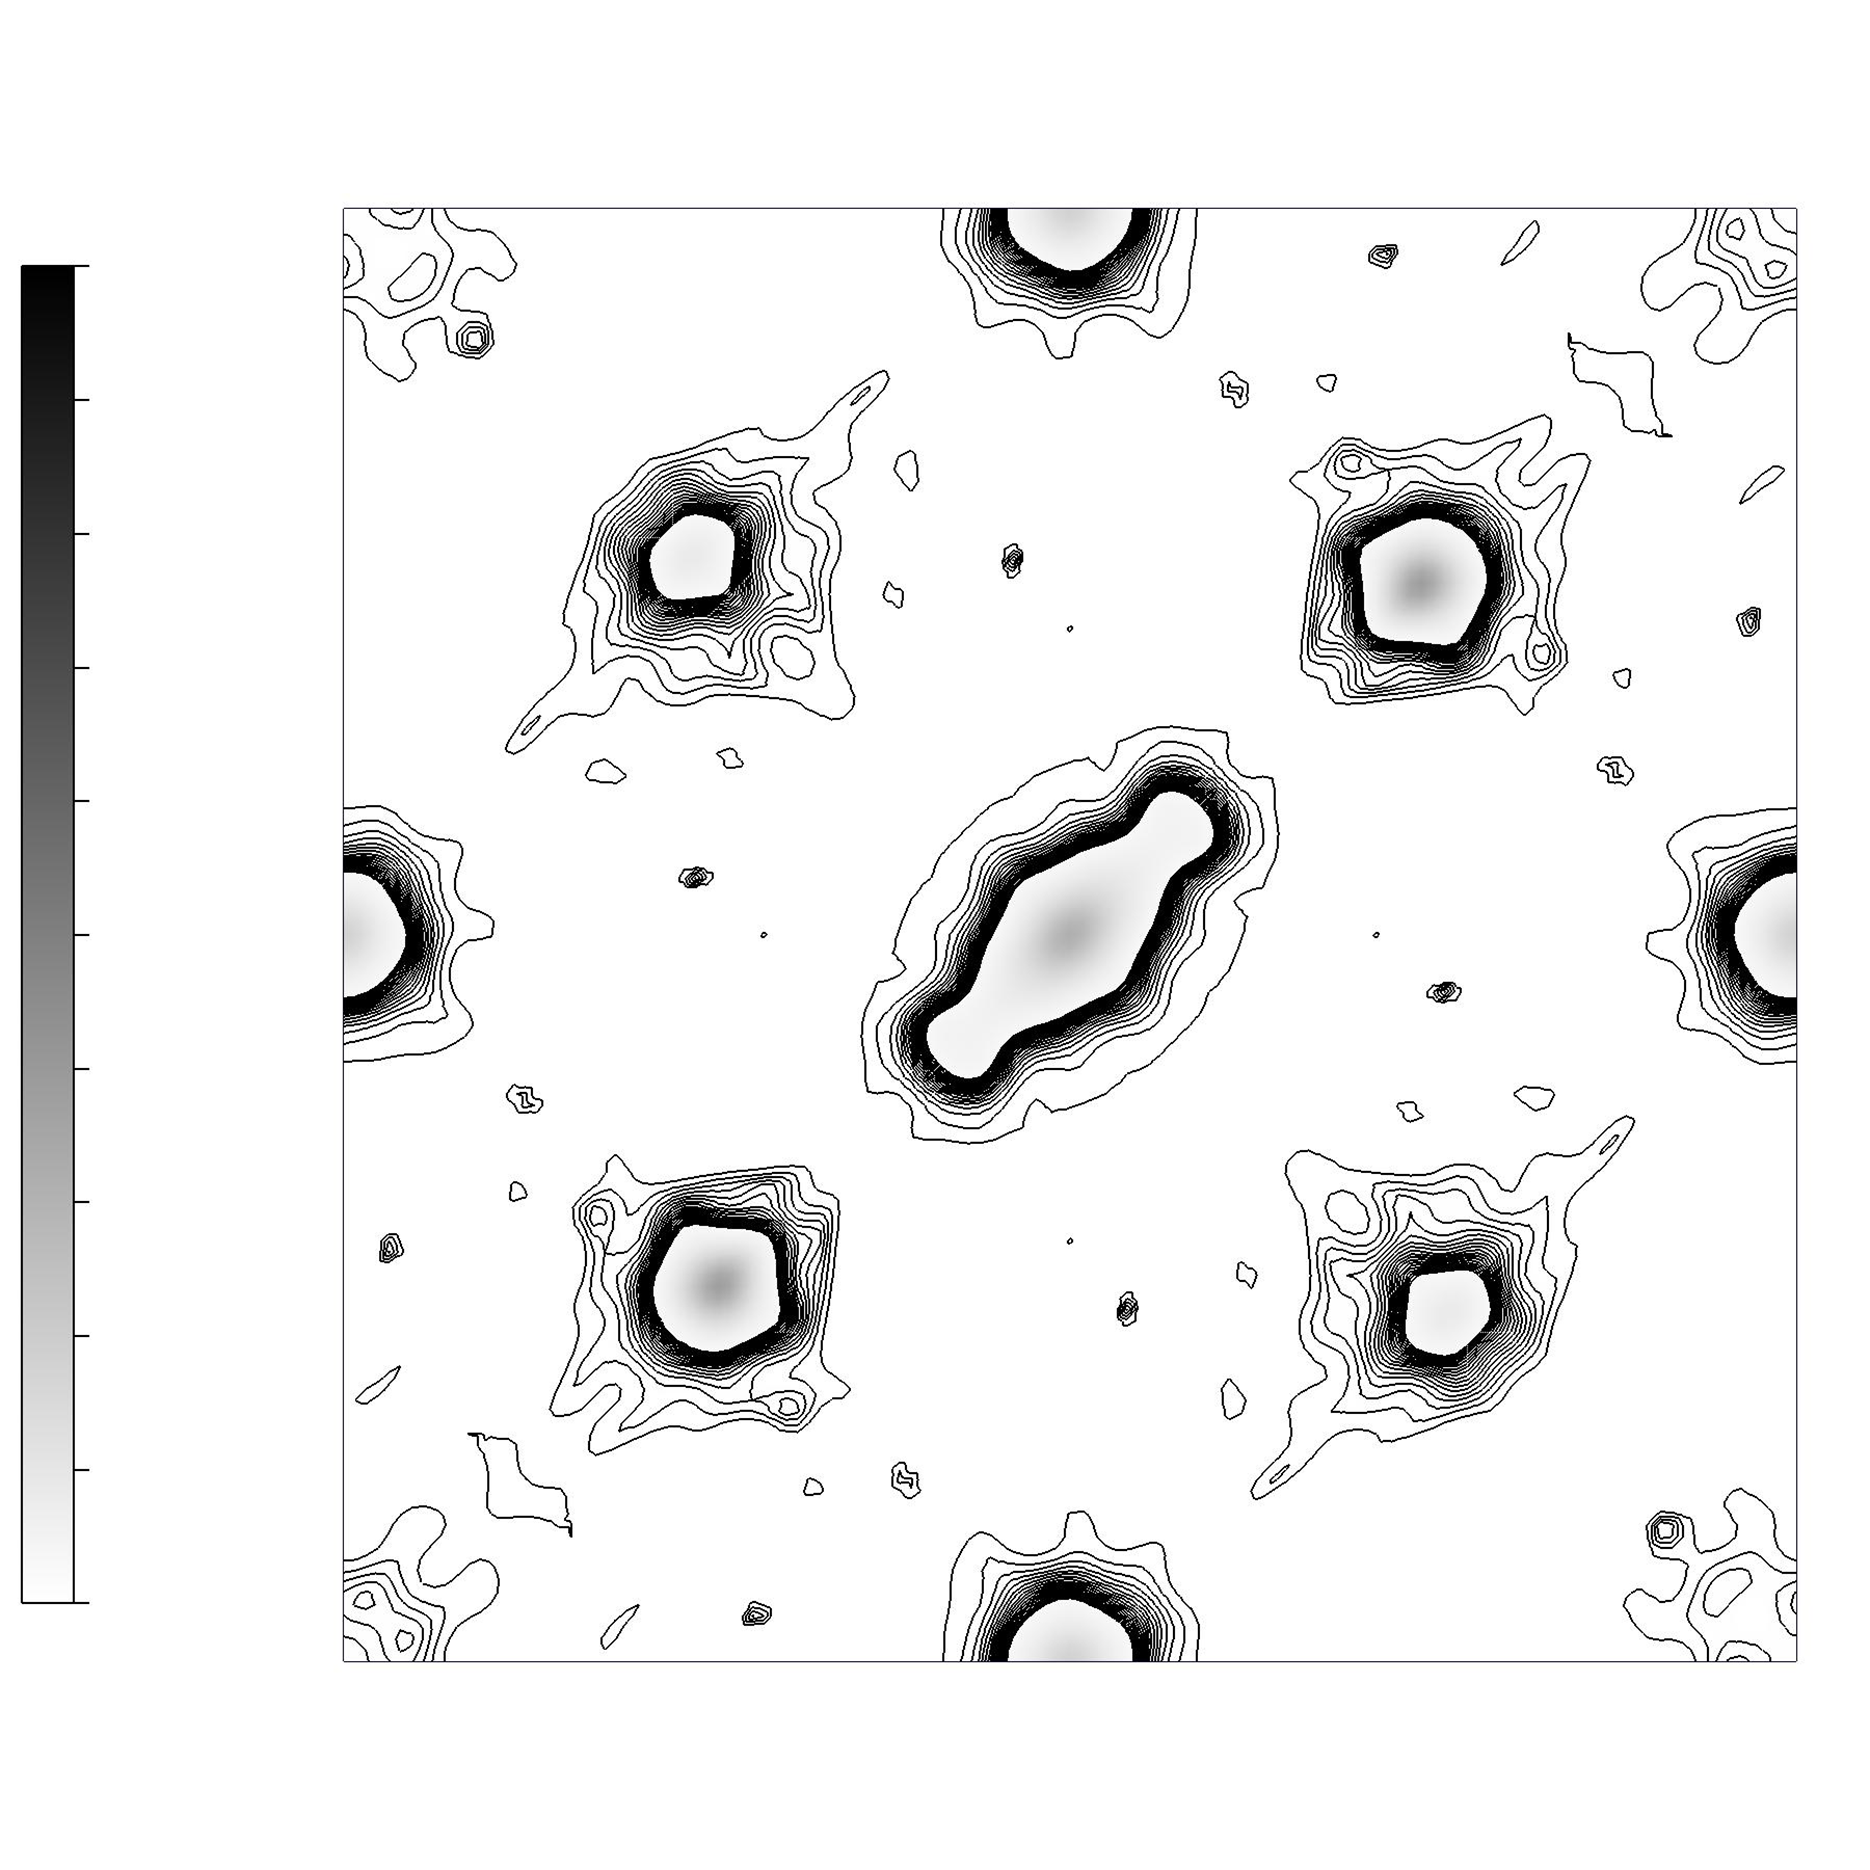
\includegraphics[width=0.9\linewidth]{Electron_density_As} \\ а)
%  \end{minipage}
%  \vfill
%  \begin{minipage}[ht]{0.7\linewidth}\centering
%    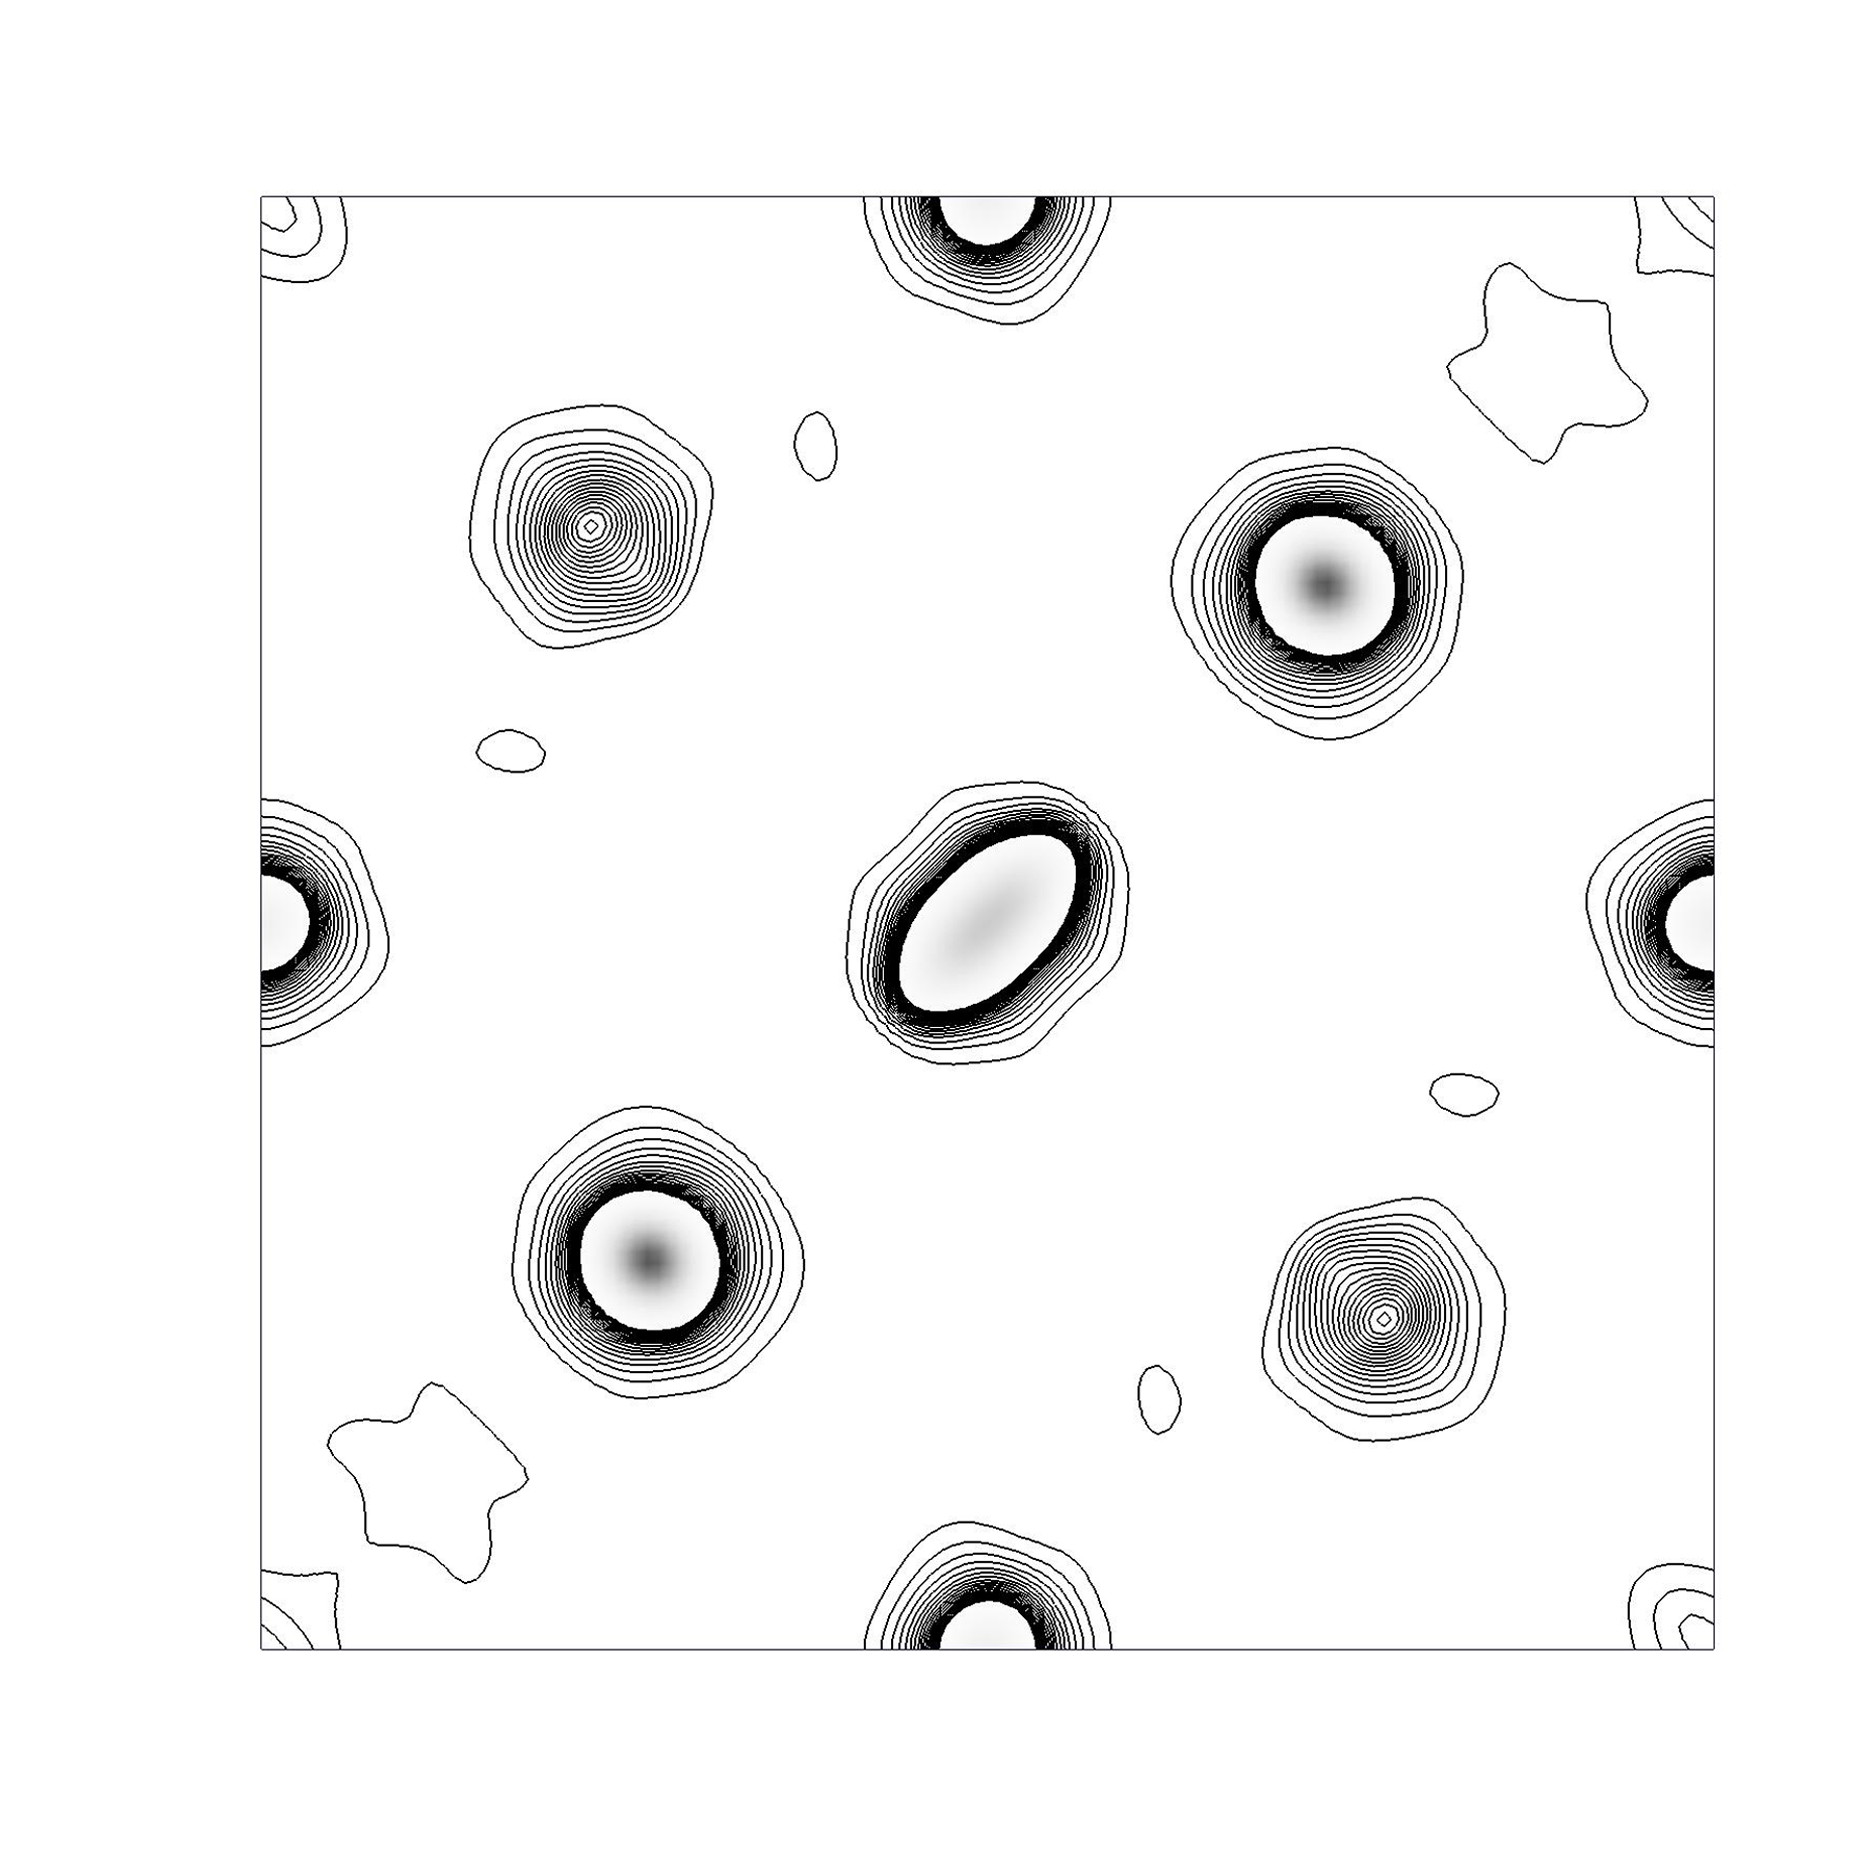
\includegraphics[width=0.9\linewidth]{Electron_density_Sb} \\ б)
%  \end{minipage}
%  \caption[Электронная плотность синтетического теннантита Cu\textsubscript{12}As\textsubscript{4}S\textsubscript{13} и тетраэдрита Cu\textsubscript{12}Sb\textsubscript{4}S\textsubscript{13}]{Электронная плотность синтетического теннантита Cu\textsubscript{12}As\textsubscript{4}S\textsubscript{13} и тетраэдрита Cu\textsubscript{12}Sb\textsubscript{4}S\textsubscript{13}}
%    \label{img:electro}
% \end{figure}

\begin{figure}[hb]
  \begin{minipage}[ht]{0.5\linewidth}\centering
    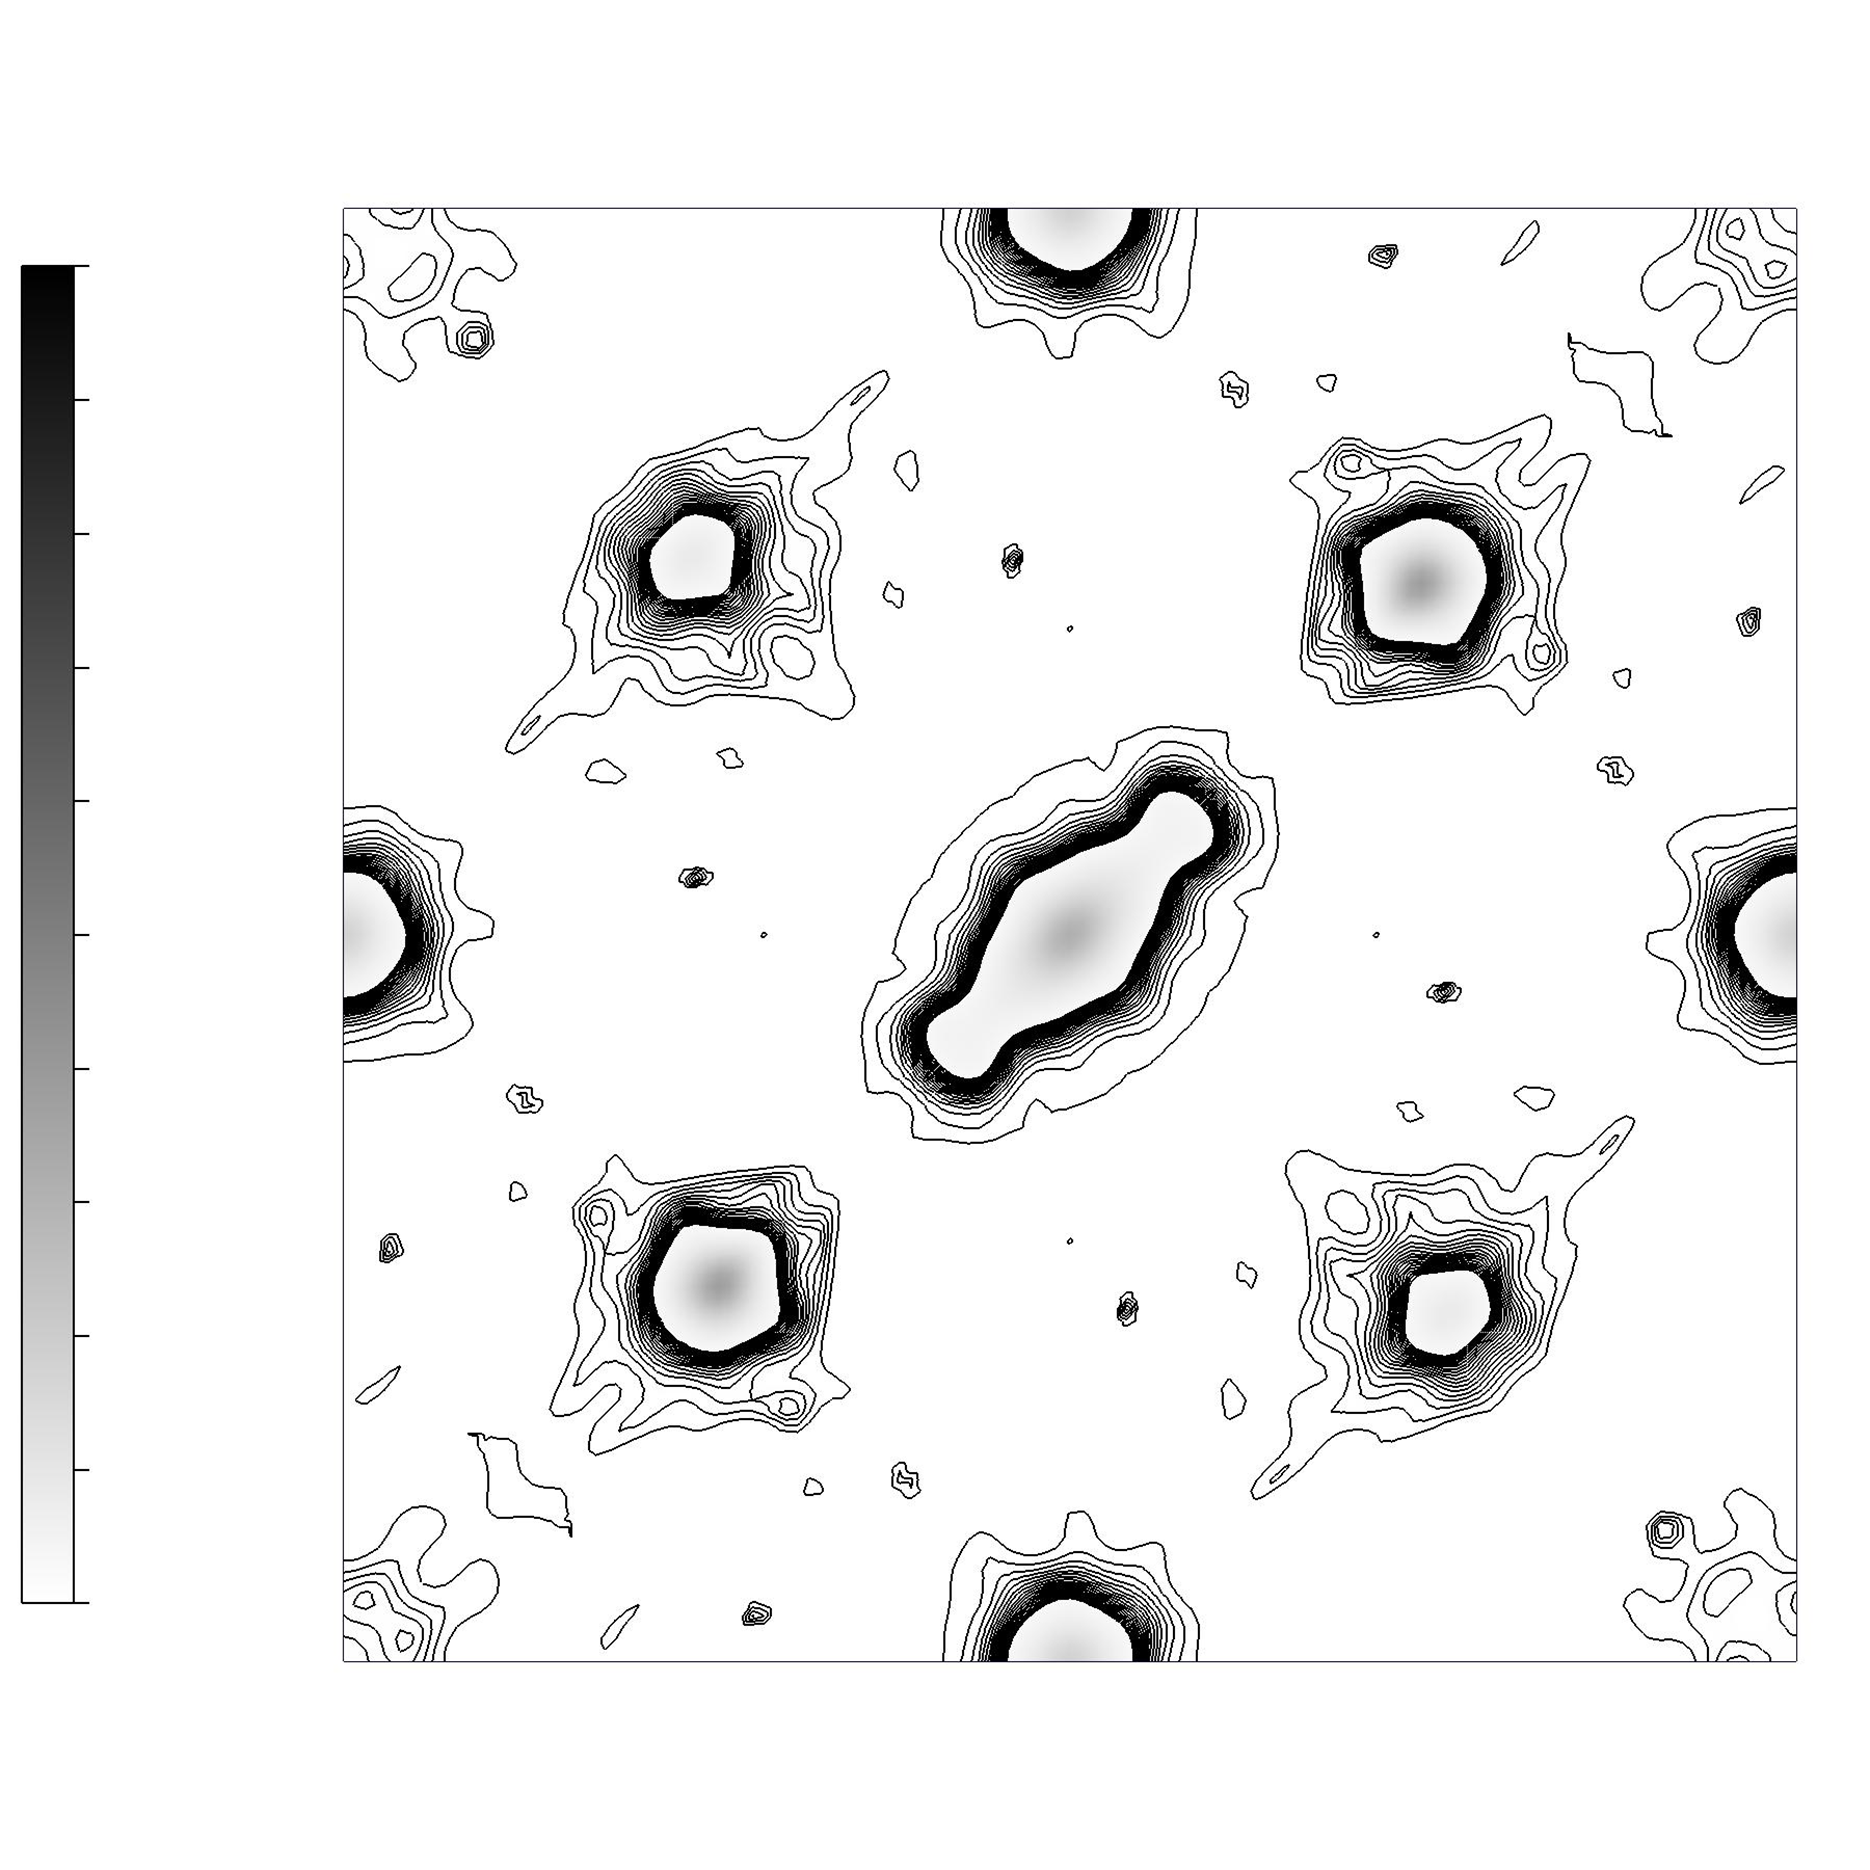
\includegraphics[width=0.9\linewidth]{Electron_density_As.png} \\ а)
  \end{minipage}
  \hfill
  \begin{minipage}[ht]{0.5\linewidth}\centering
    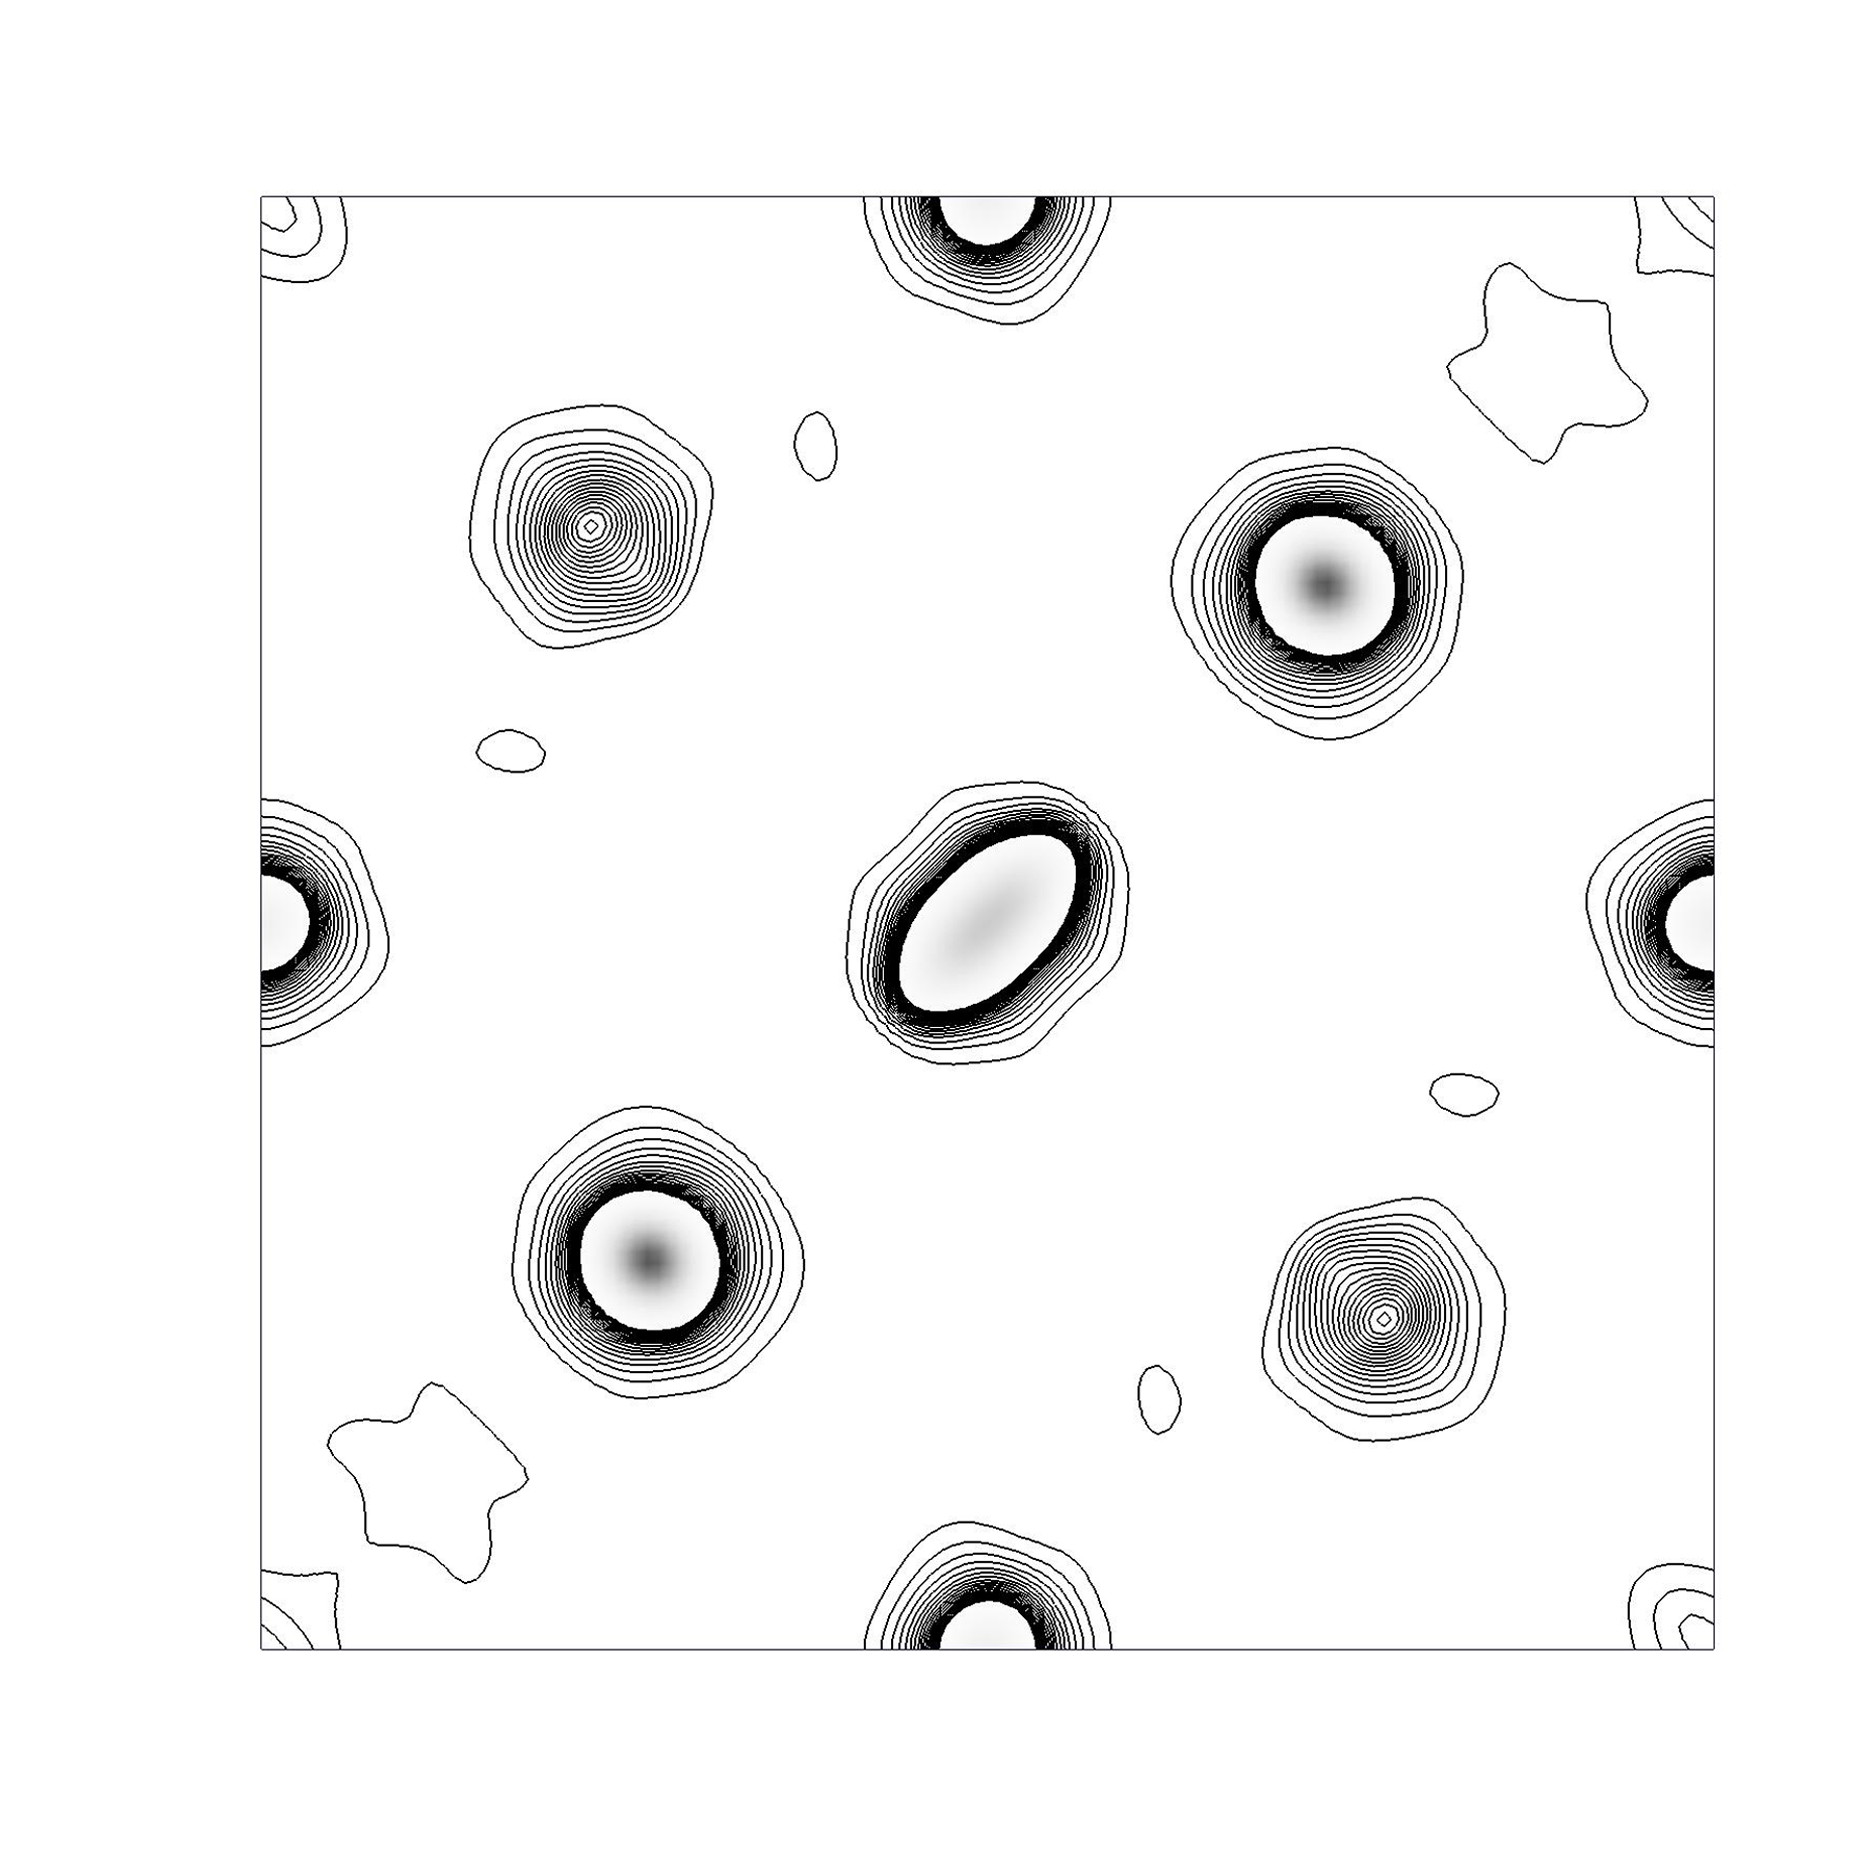
\includegraphics[width=0.9\linewidth]{Electron_density_Sb.png} \\ б)
  \end{minipage}

 \caption[Электронная плотность синтетического теннантита Cu\textsubscript{12}As\textsubscript{4}S\textsubscript{13}(а) и тетраэдрита Cu\textsubscript{12}Sb\textsubscript{4}S\textsubscript{13}(б)]{Электронная плотность синтетического теннантита Cu\textsubscript{12}As\textsubscript{4}S\textsubscript{13}(а) и тетраэдрита Cu\textsubscript{12}Sb\textsubscript{4}S\textsubscript{13}(б)}
   \label{img:electro}
\end{figure}

\begin{figure}[p!]
  \begin{minipage}[ht]{0.9\linewidth}\centering
    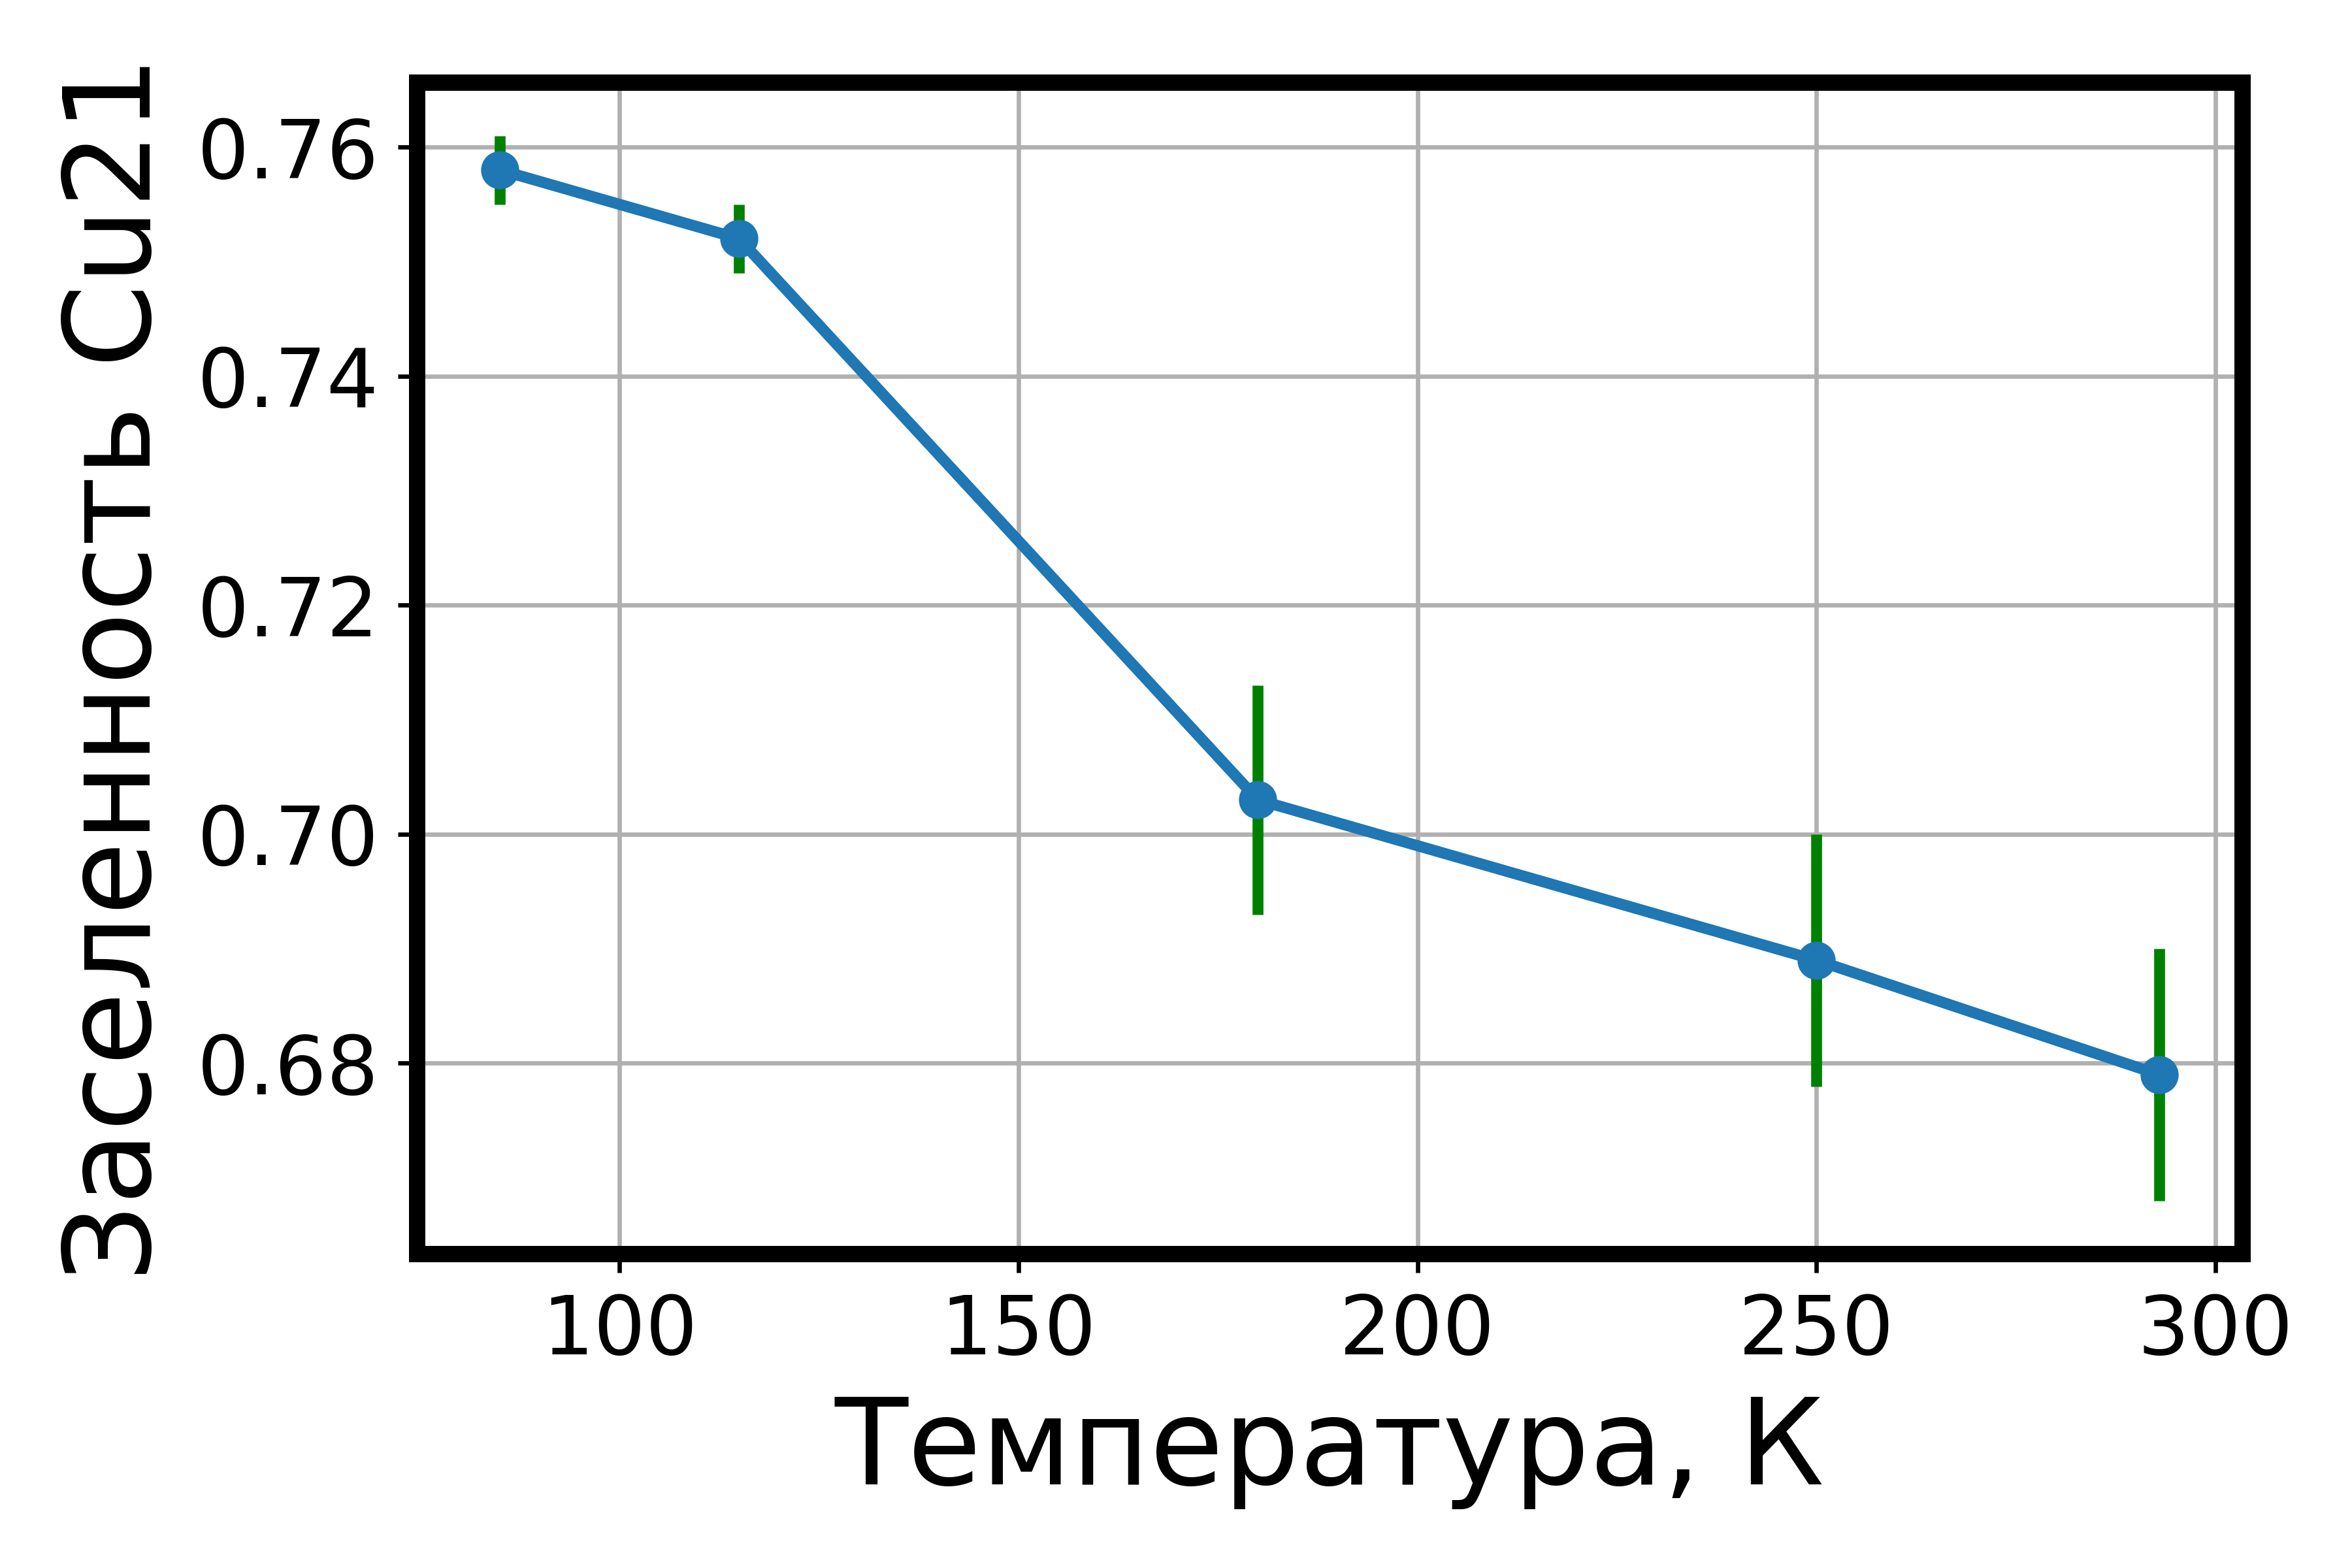
\includegraphics[width=0.9\linewidth]{structure_occCu2} \\ а)
  \end{minipage}
  \vfill
  \begin{minipage}[ht]{0.9\linewidth}\centering
    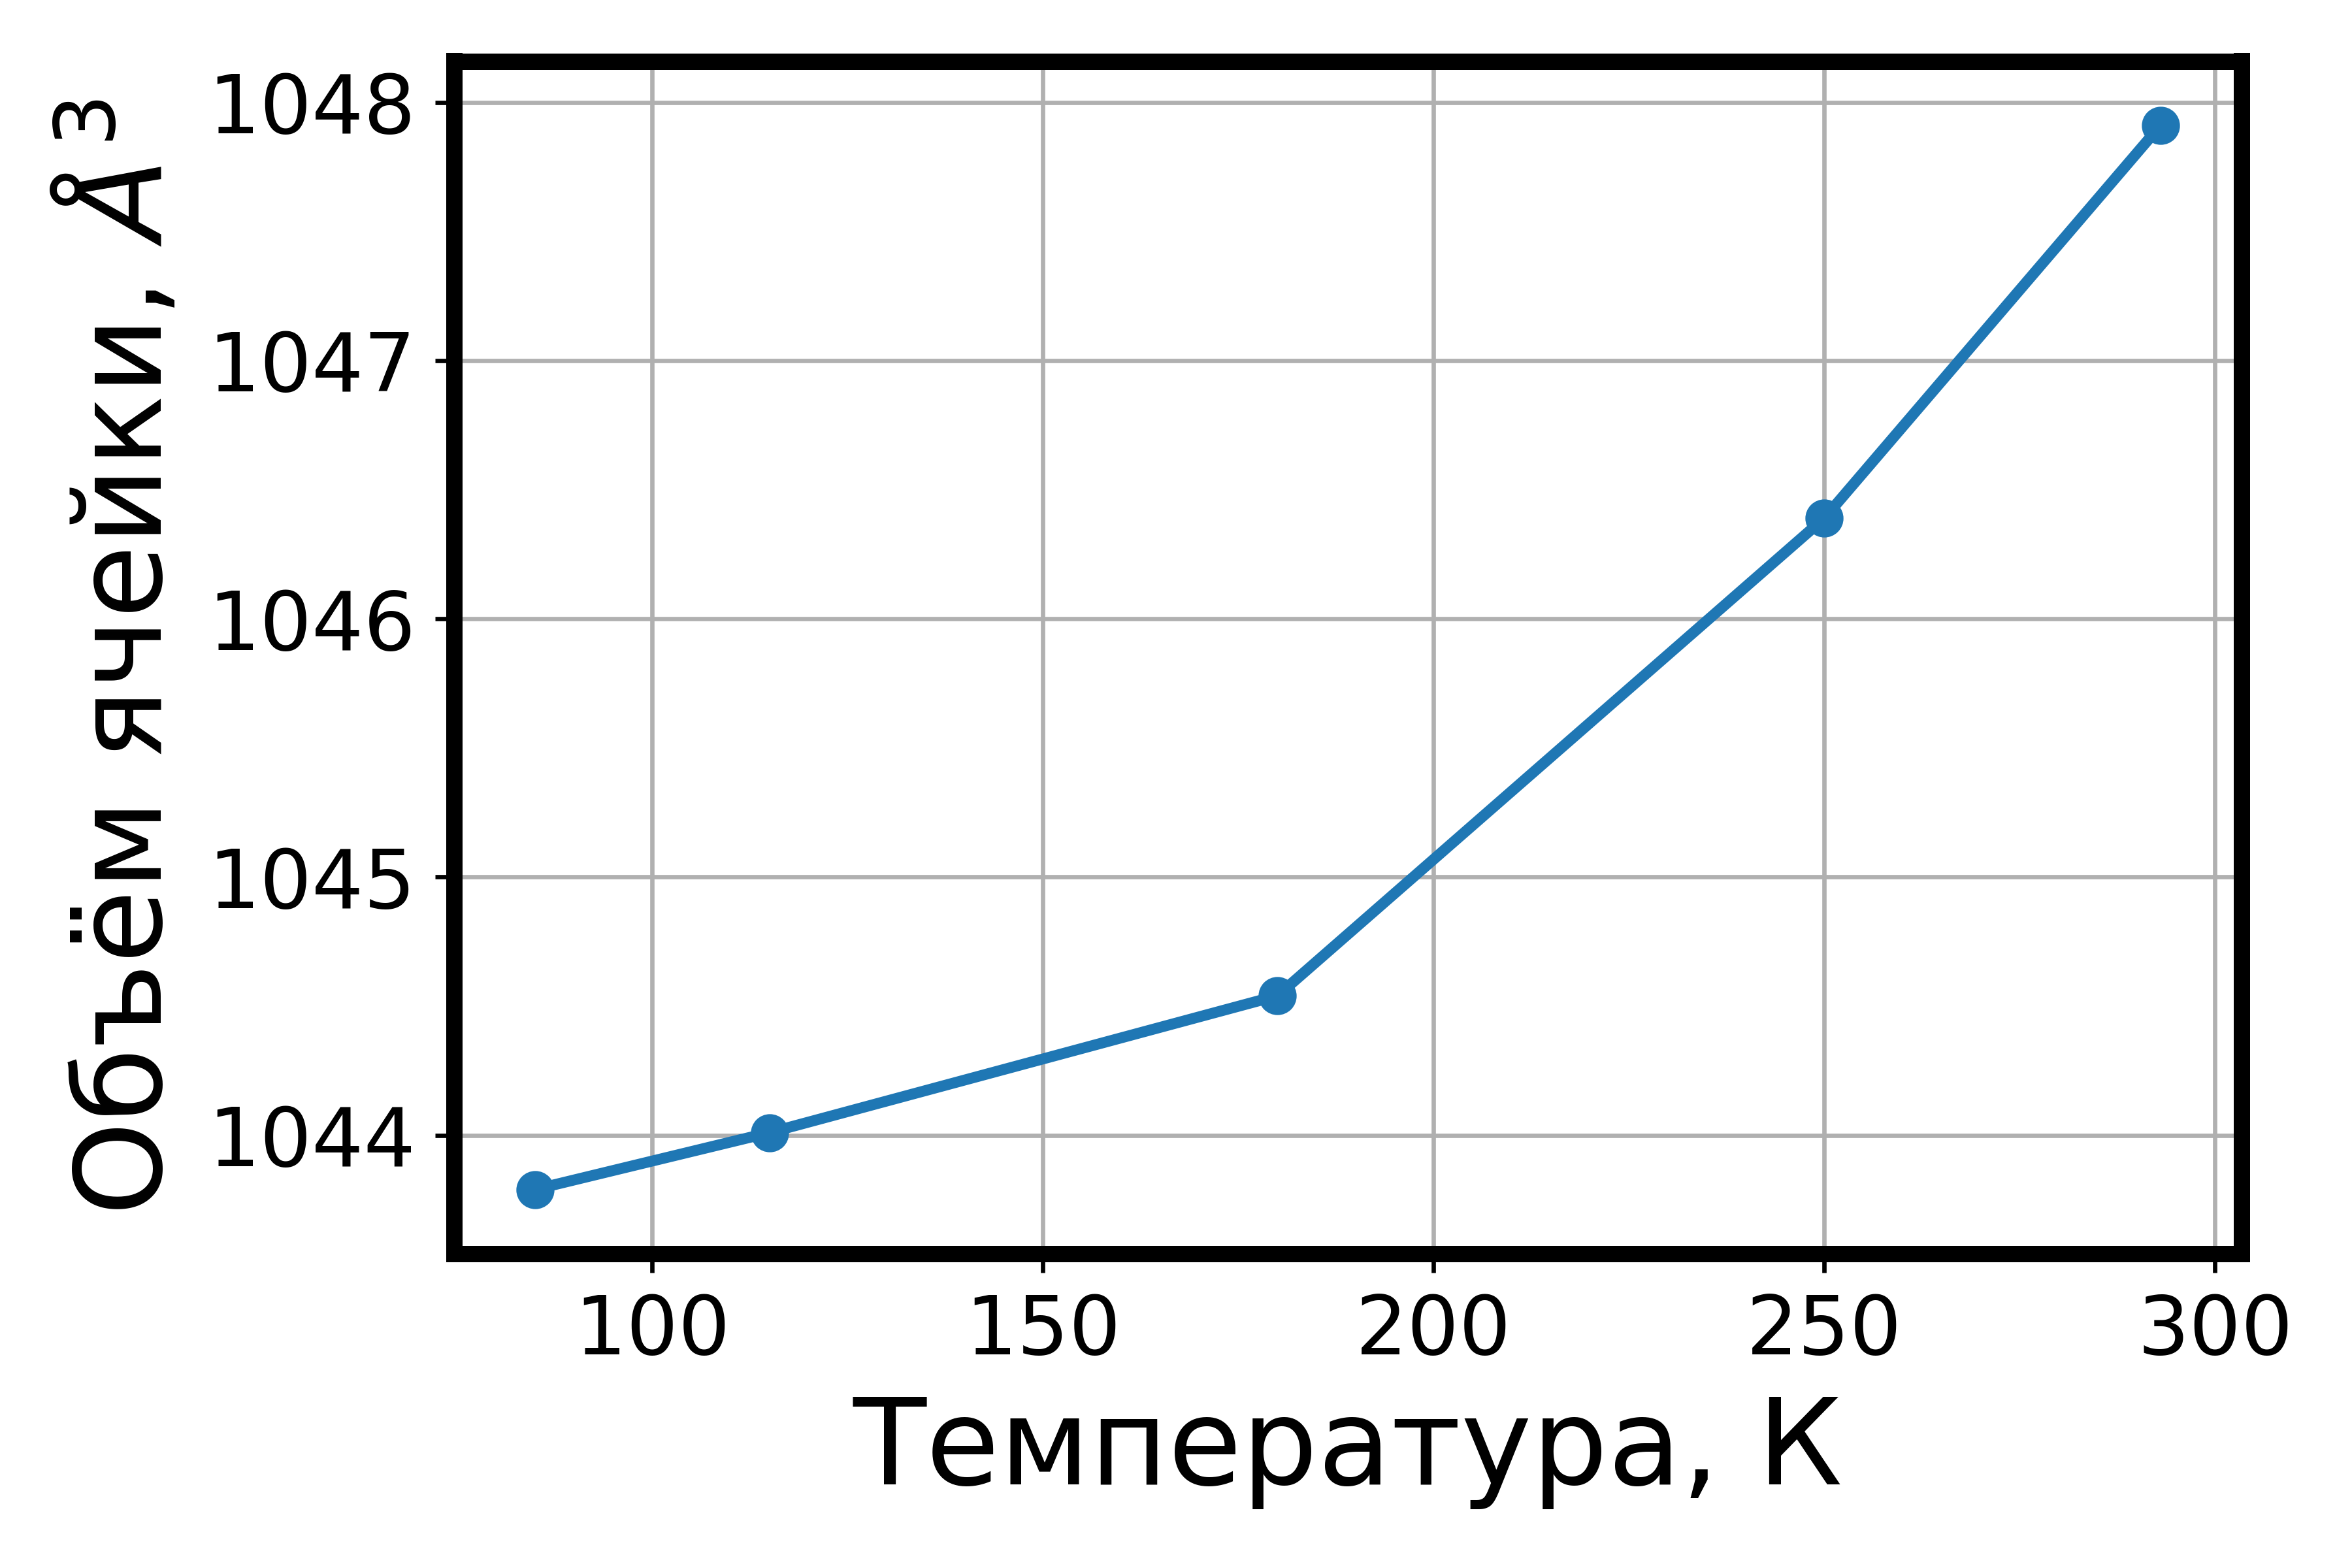
\includegraphics[width=0.9\linewidth]{structure_volume} \\ б)
  \end{minipage}

      \caption[Зависимости изменения заселённости для позиции Cu21(а) и объёма кристаллической решетки (б) образца синтетического теннантита Cu\textsubscript{12}As\textsubscript{4}S\textsubscript{13} от температуры]{Зависимости изменения заселённости для позиции Cu21(а) и объёма кристаллической решетки (б) образца синтетического теннантита Cu\textsubscript{12}As\textsubscript{4}S\textsubscript{13} от температуры}
    \label{img:structure1}
\end{figure}

\begin{figure}[p!]
  \begin{minipage}[ht]{0.9\linewidth}\centering
    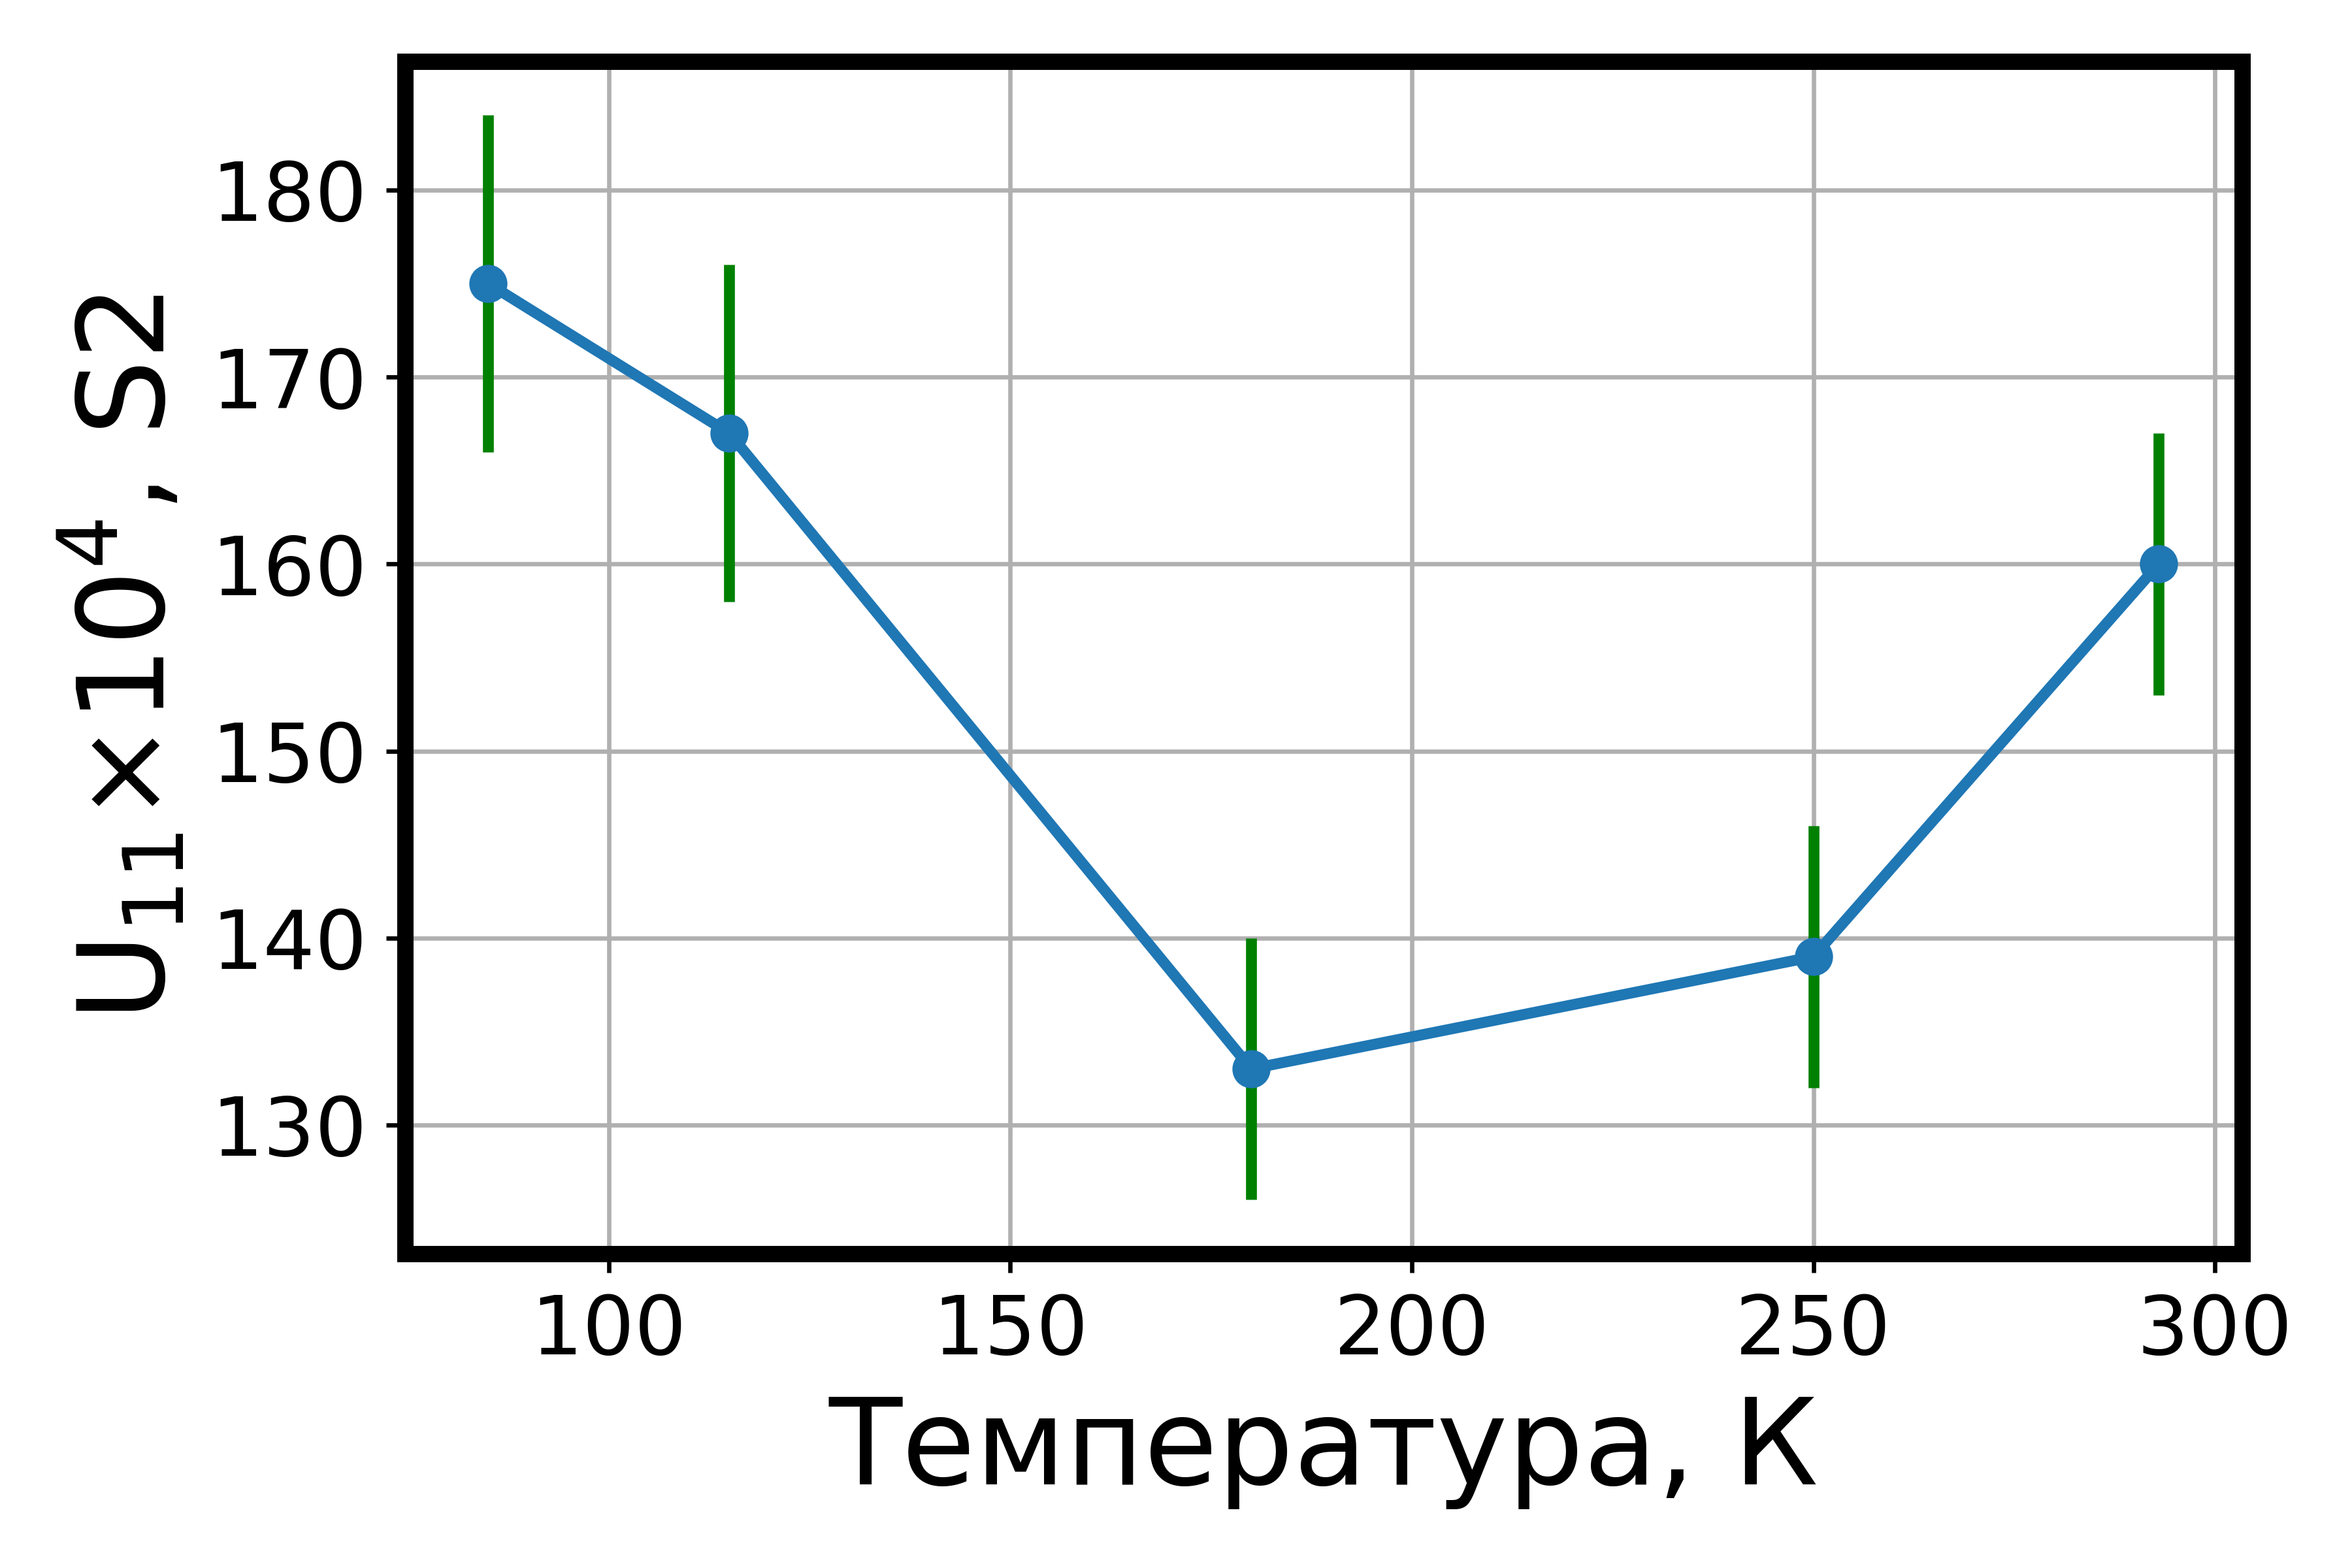
\includegraphics[width=0.9\linewidth]{structure_Ueq} \\ а)
  \end{minipage}
  \vfill
  \begin{minipage}[ht]{0.9\linewidth}\centering
    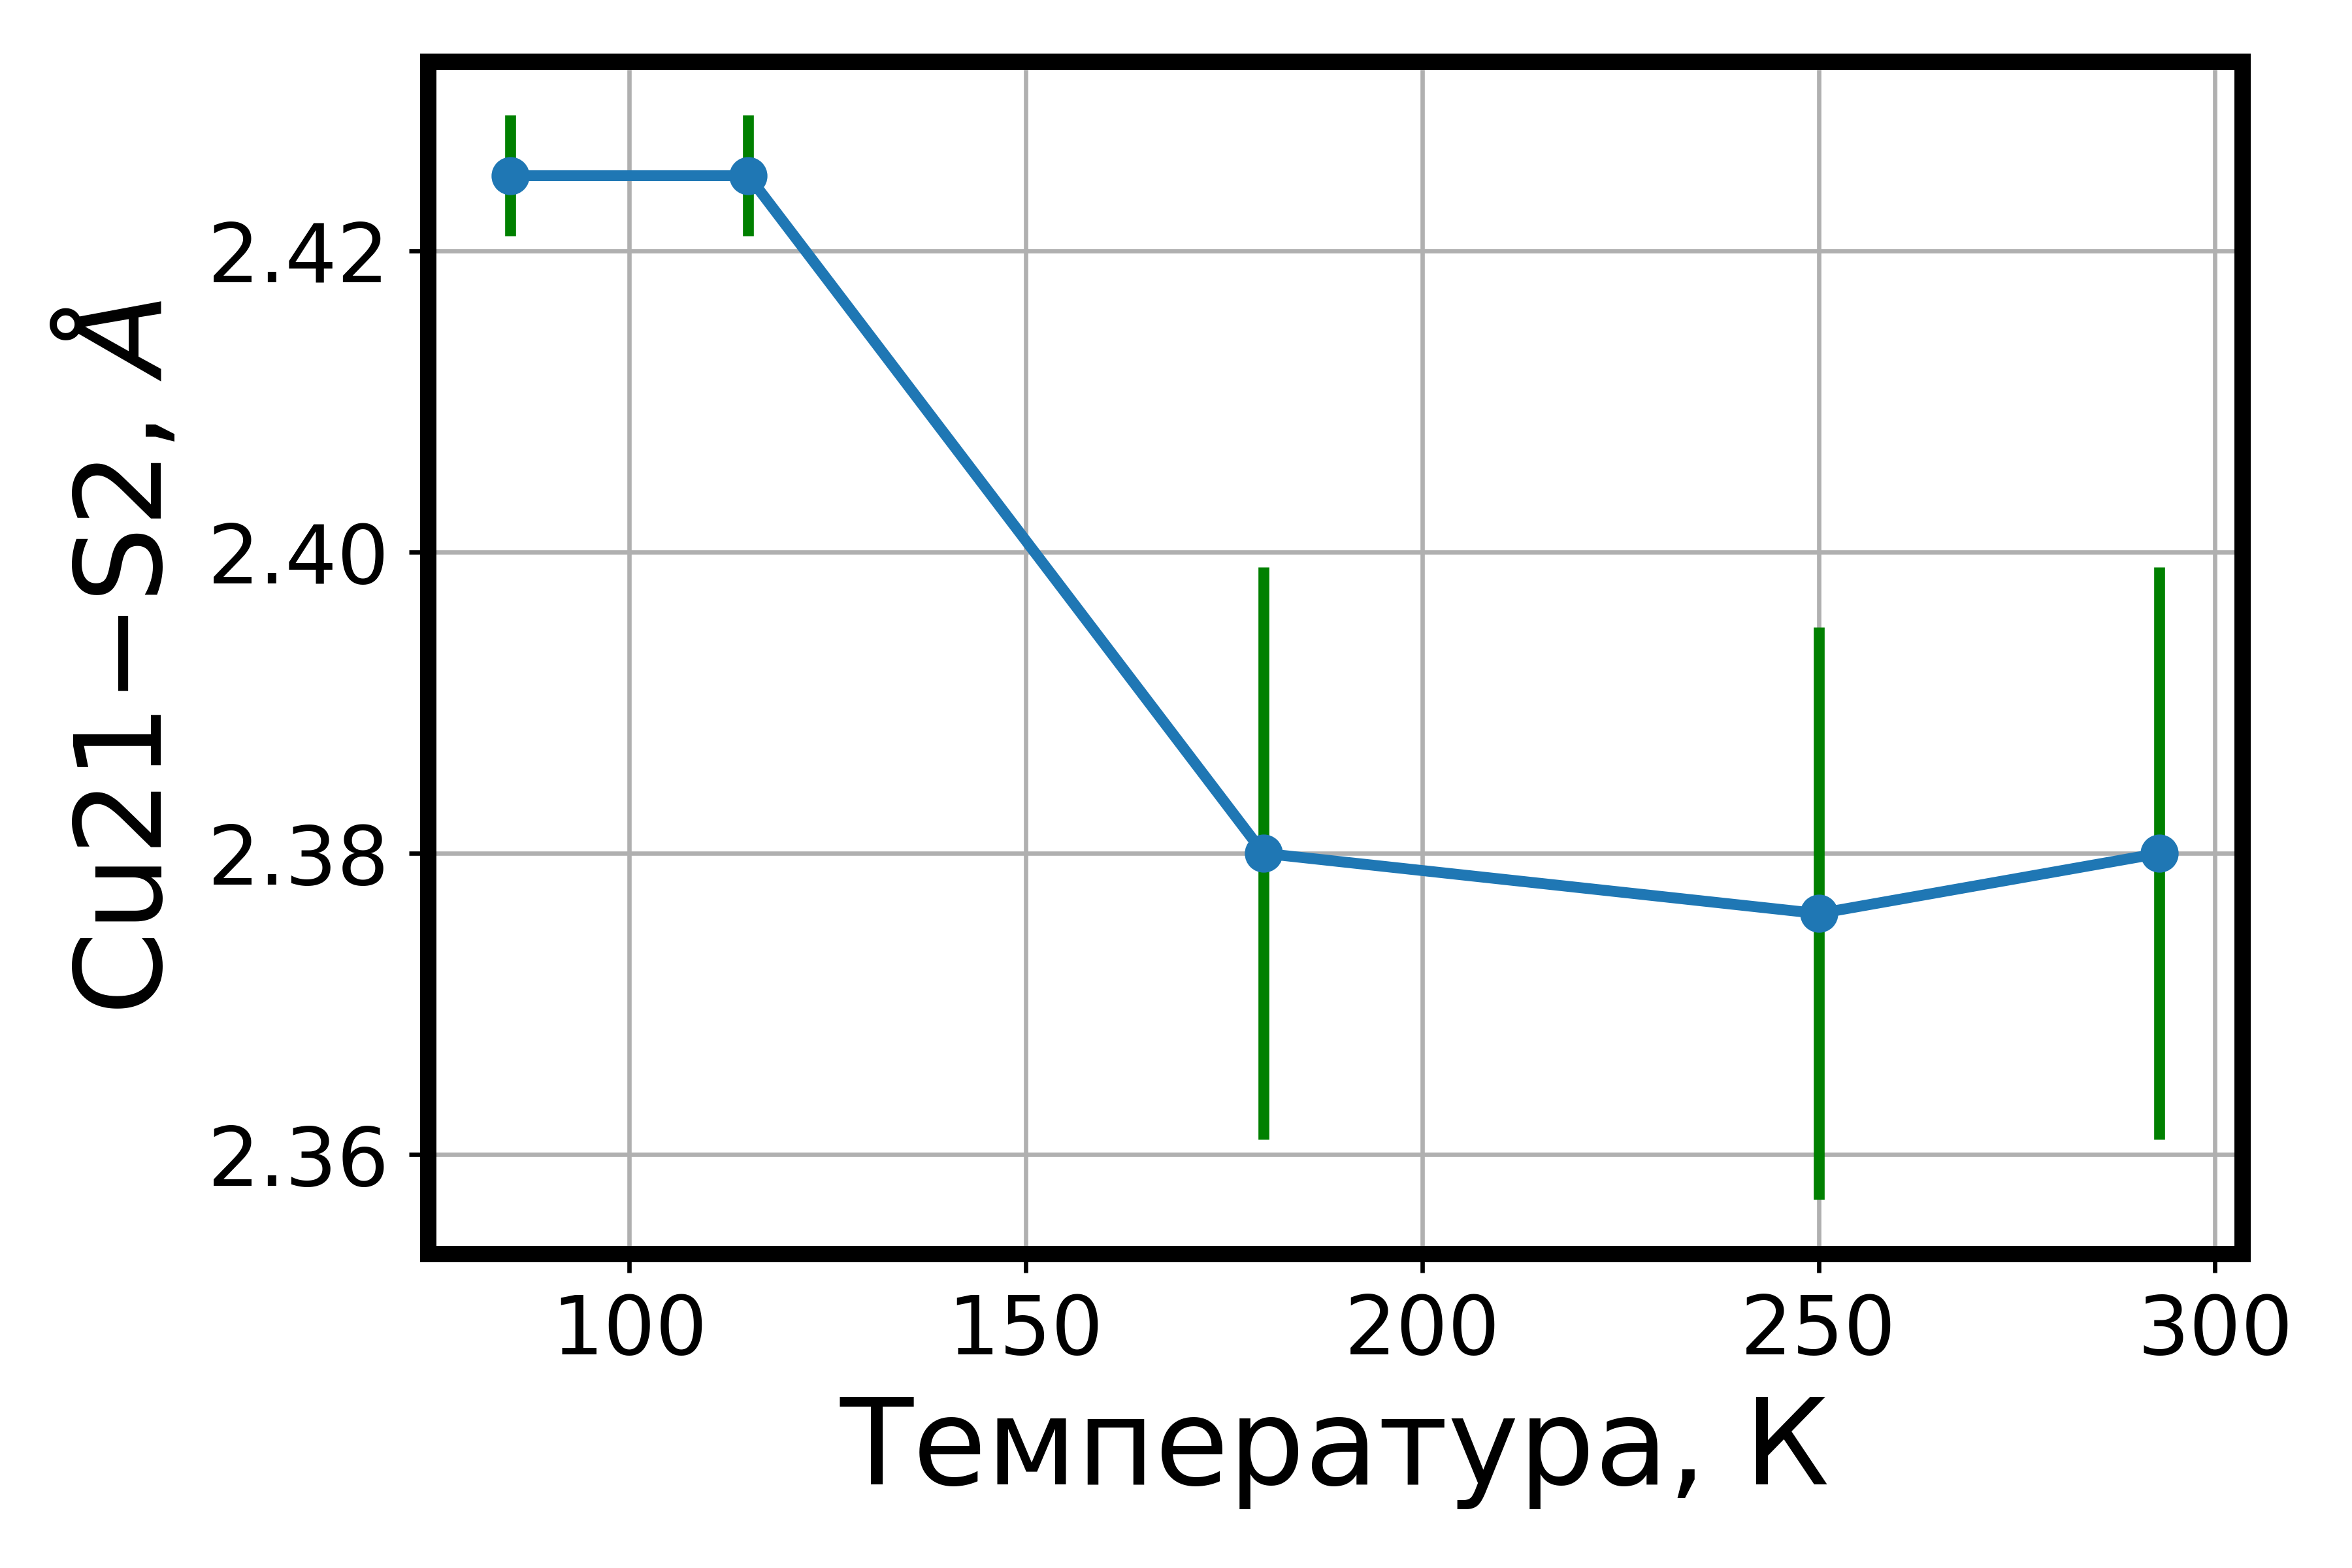
\includegraphics[width=0.9\linewidth]{structure_cu21_s2} \\ б)
  \end{minipage}

      \caption[Зависимости атомарного смещения U\textsubscript{11} (а) и расстояния между позициями Cu21--S2 (б) для образца синтетического теннантита Cu\textsubscript{12}As\textsubscript{4}S\textsubscript{13} от температуры]{Зависимости атомарного смещения U\textsubscript{11} (а) и расстояния между позициями Cu21--S2 (б) для образца синтетического теннантита Cu\textsubscript{12}As\textsubscript{4}S\textsubscript{13} от температуры}
    \label{img:structure2}
\end{figure}
\newpage

\section{Электронная просвечивающая микроскопия монокристаллического образца синтетического теннантита Cu\textsubscript{12}As\textsubscript{4}S\textsubscript{13} в плоскости (011) } \label{sect3_2}

Исследования особенностей распределения меди в образце проведены при комнатной температуре на образце толщиной менее 100~нм для кристаллографической плоскости (011).
Установлено, что в образце синтетического теннантита Cu\textsubscript{12}As\textsubscript{4}S\textsubscript{13} есть различия значения эллиптичности в рядах меди Cu (Рис. \ref{img:mic}).

\begin{figure}[h!]
  \begin{minipage}[ht]{0.9\linewidth}\centering
    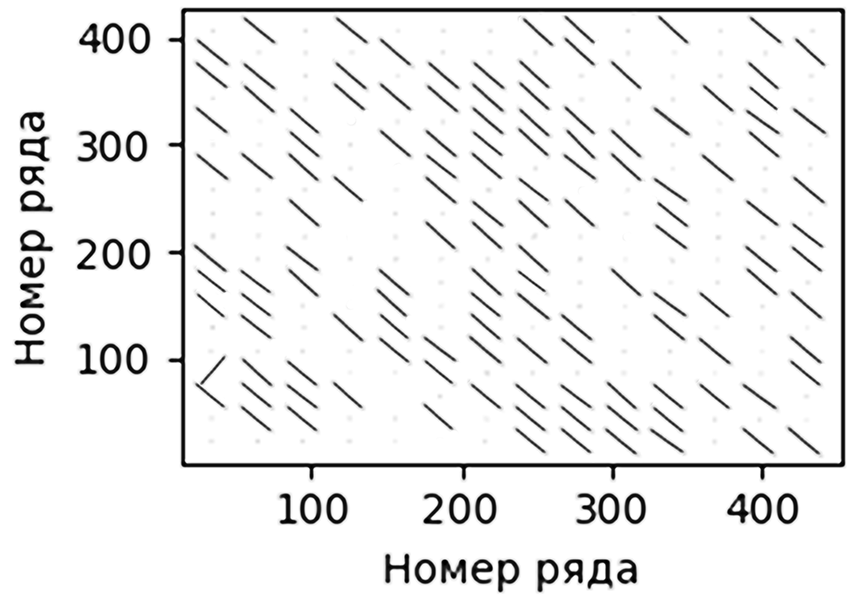
\includegraphics[width=0.7\linewidth]{mic_cupper_raw}
  \end{minipage}

      \caption[Величина и разворот эллиптичности рядов Cu в кристаллографической плоскости (011) синтетического теннантита Cu\textsubscript{12}As\textsubscript{4}S\textsubscript{13}]{Величина и разворот эллиптичности рядов Cu в кристаллографической плоскости (011) синтетического теннантита Cu\textsubscript{12}As\textsubscript{4}S\textsubscript{13}}
    \label{img:mic}
\end{figure}


На рисунке \ref{img:mic2} электронная дифракция для плоскости (011) образца синтетического образца Cu\textsubscript{12}As\textsubscript{4}S\textsubscript{13}.
Дифракция демонстрирует чётко определяемые рефлексы, которые хорошо идентифицируются (рис. \ref{img:mic2}(б)).

\begin{figure}[ph!]
\centering
  \begin{minipage}[ht]{0.7\linewidth}\centering
    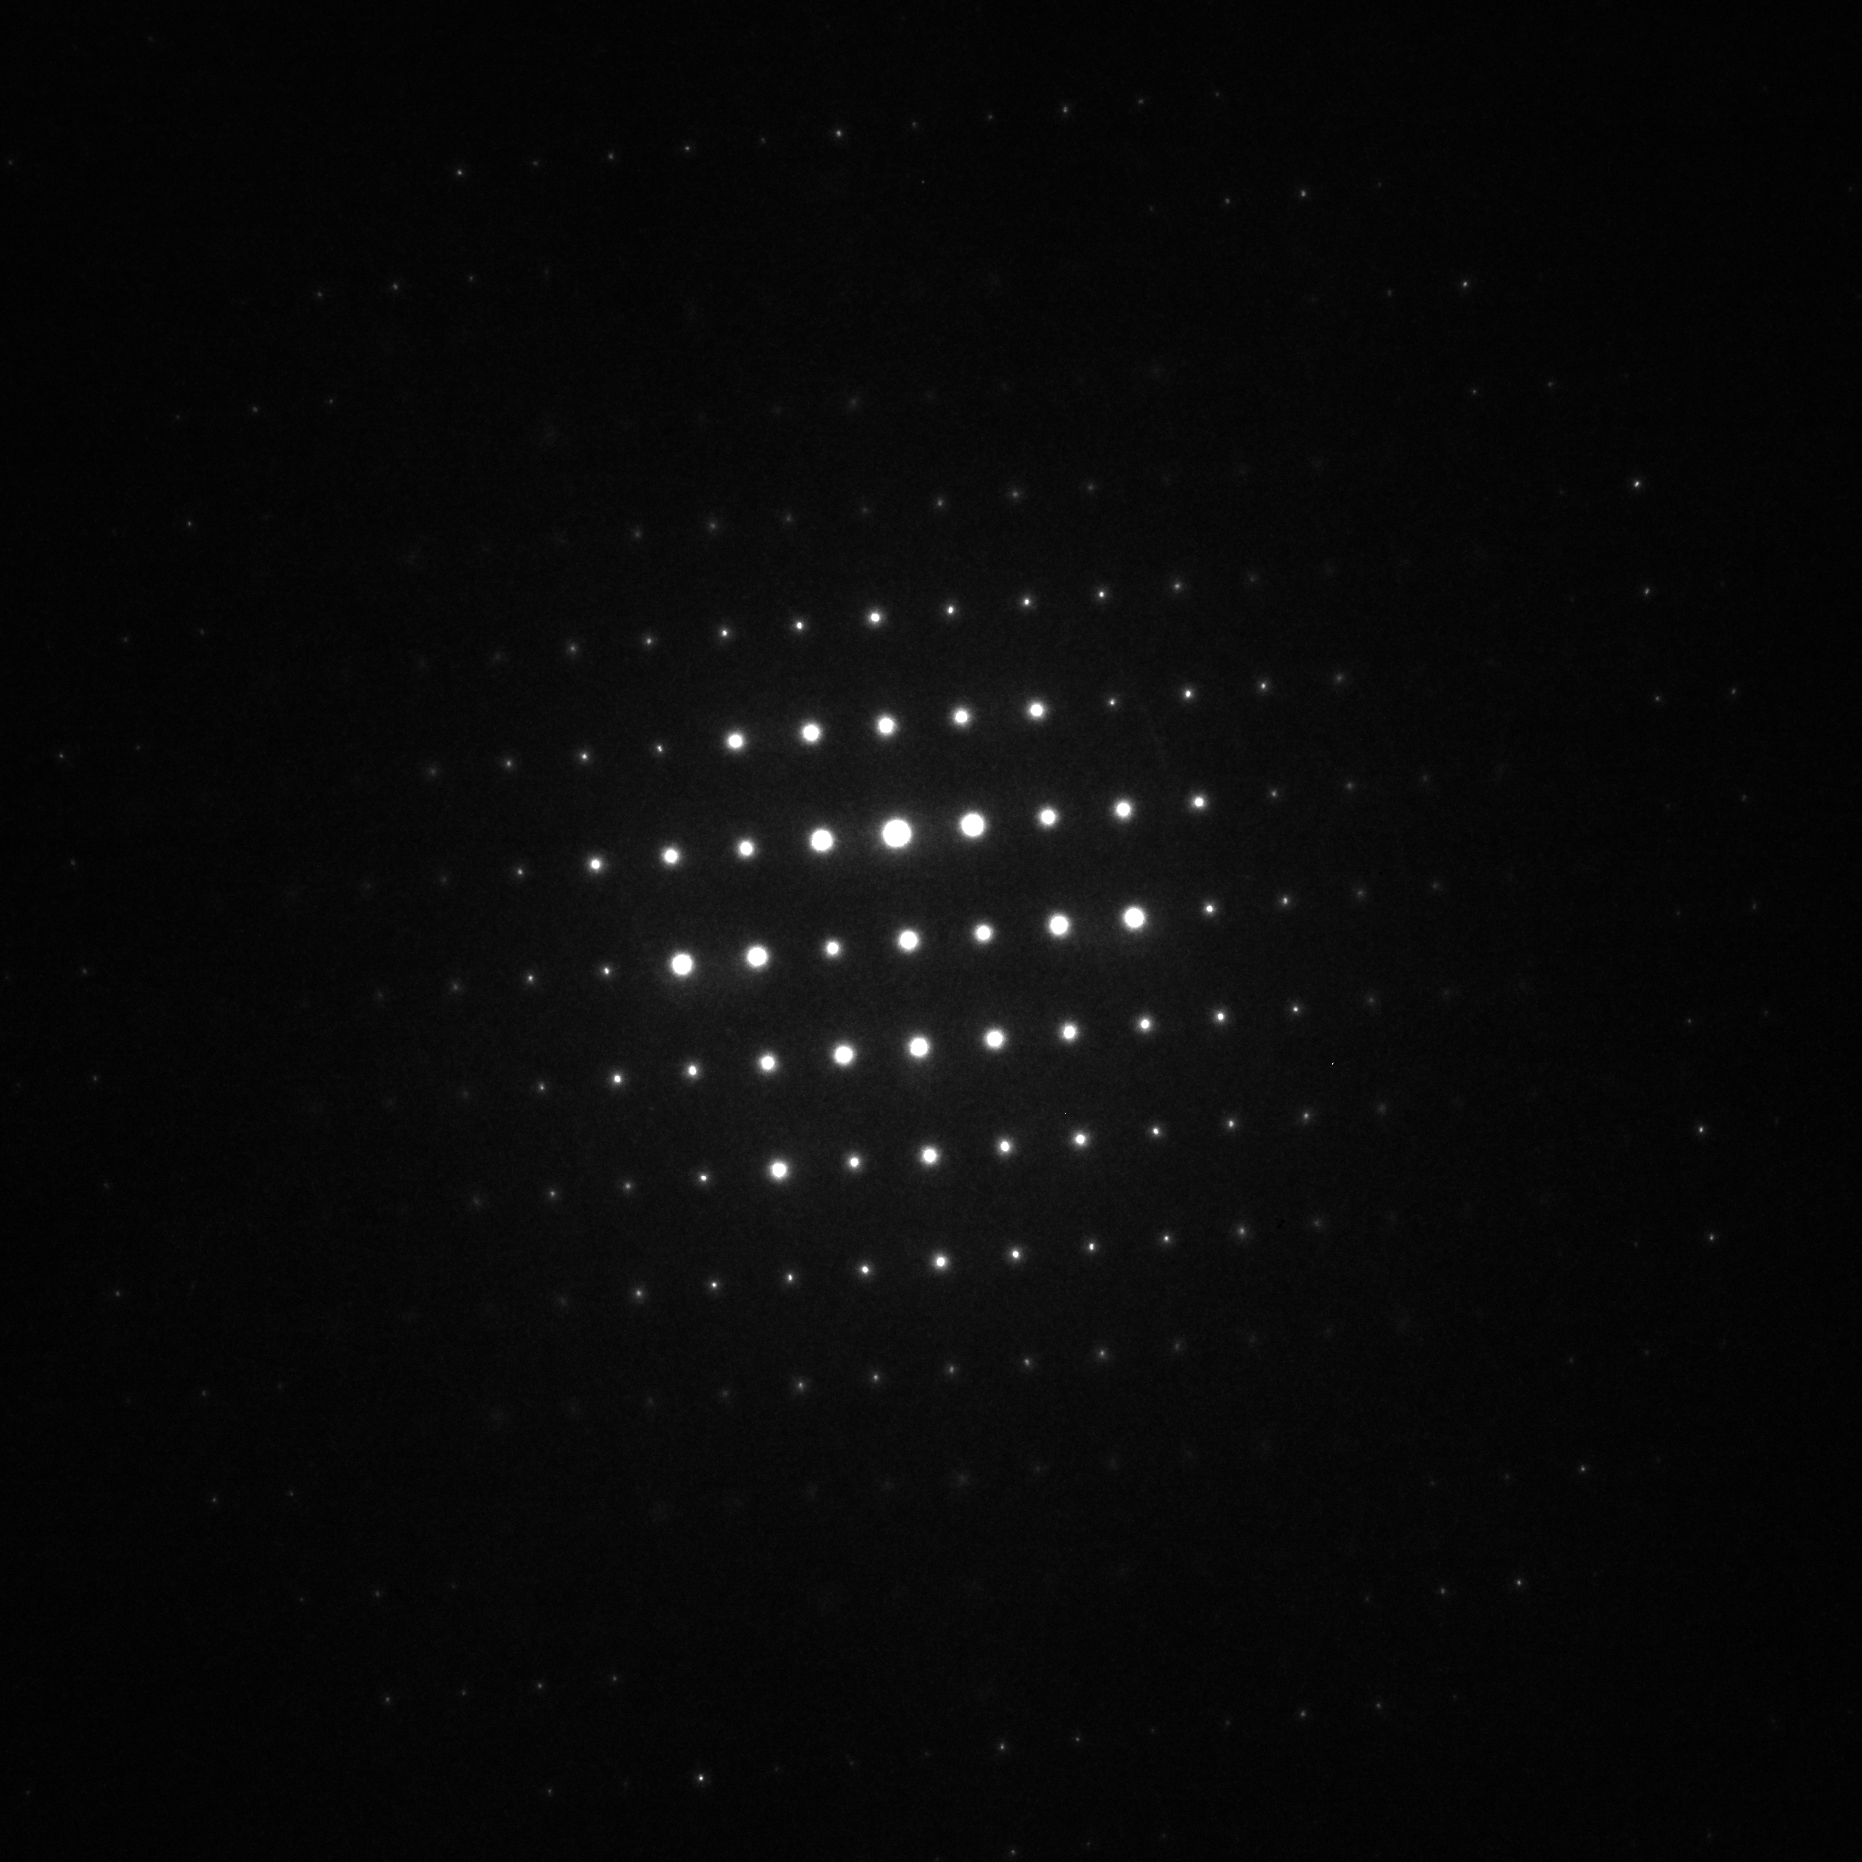
\includegraphics[width=0.9\linewidth]{difr01_el_mic} \\ а)
  \end{minipage}
  \vfill
  \begin{minipage}[ht]{0.7\linewidth}\centering
    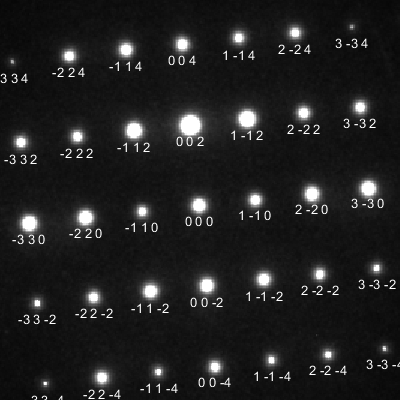
\includegraphics[width=0.9\linewidth]{difr01_el_mic_zone_110} \\ б)
  \end{minipage}
  \caption[Электронная дифракция для плоскости (011) для образца Cu\textsubscript{12}As\textsubscript{4}S\textsubscript{13}. Оригинальное изображение (а) и изображение с отмеченными дифракционными рефлексами (б)]{Электронная дифракция для плоскости (011) для образца Cu\textsubscript{12}As\textsubscript{4}S\textsubscript{13}. Оригинальное изображение (а) и изображение с отмеченными дифракционными рефлексами (б)}
    \label{img:mic2}
\end{figure}

Анализ изображения структуры показывает наличие разной эллиптичности для рядов атомов меди. На рисунке \ref{img:mic} представлено наличие эллиптичности атомов рядов меди с учётом дрейфа для плоскости (011) синтетического теннантита Cu\textsubscript{12}As\textsubscript{4}S\textsubscript{13}.




\newpage



\section{Комбинационное рассеяние света синтетического теннантита Cu\textsubscript{12}As\textsubscript{4}S\textsubscript{13}} \label{sect3_3}

Спектр комбинационного рассеяния для синтетического теннантита обладает низкоэнергетическими модами (Рис. \ref{img:raman1a}).

Спектр комбинационного рассеяния света состоит из следующих пиков: $\nu_{1}$, $\nu_{2}$, $l_{1}$, $l_{2}$ на 374.5, 340, 64, и 122 см\textsuperscript{-1} соответсвенно, и широкого пика $\nu_{4}$ на 320 см\textsuperscript{-1}. Пики между 200 и 400 см\textsuperscript{-1} относят к модам от (Sb, As)S\textsubscript{3}\cite{Kharbish2007}. Позиция пика $\nu_{3}$ найдена методом наименьших квадратов с помощью пакета LMFIT.
Результаты моделирования представлены пунктиром на Рис. \ref{img:raman1a}.
Определенные по экспериментальным спектрам волновые числа и полуширина пиков ниже 200 см\textsuperscript{-1} для синтетического теннантита составляют 62(14) и 122(24) см\textsuperscript{-1}.  По мнению авторов \cite{Buzatu2017}, эти моды связаны с особенностями динамики кристаллической решетки.

Определение положения  и  полуширины пика проведено с помощью функции псевдо-Фойгта, а фон описывался полиномной функцией.

\begin{figure}[h]
    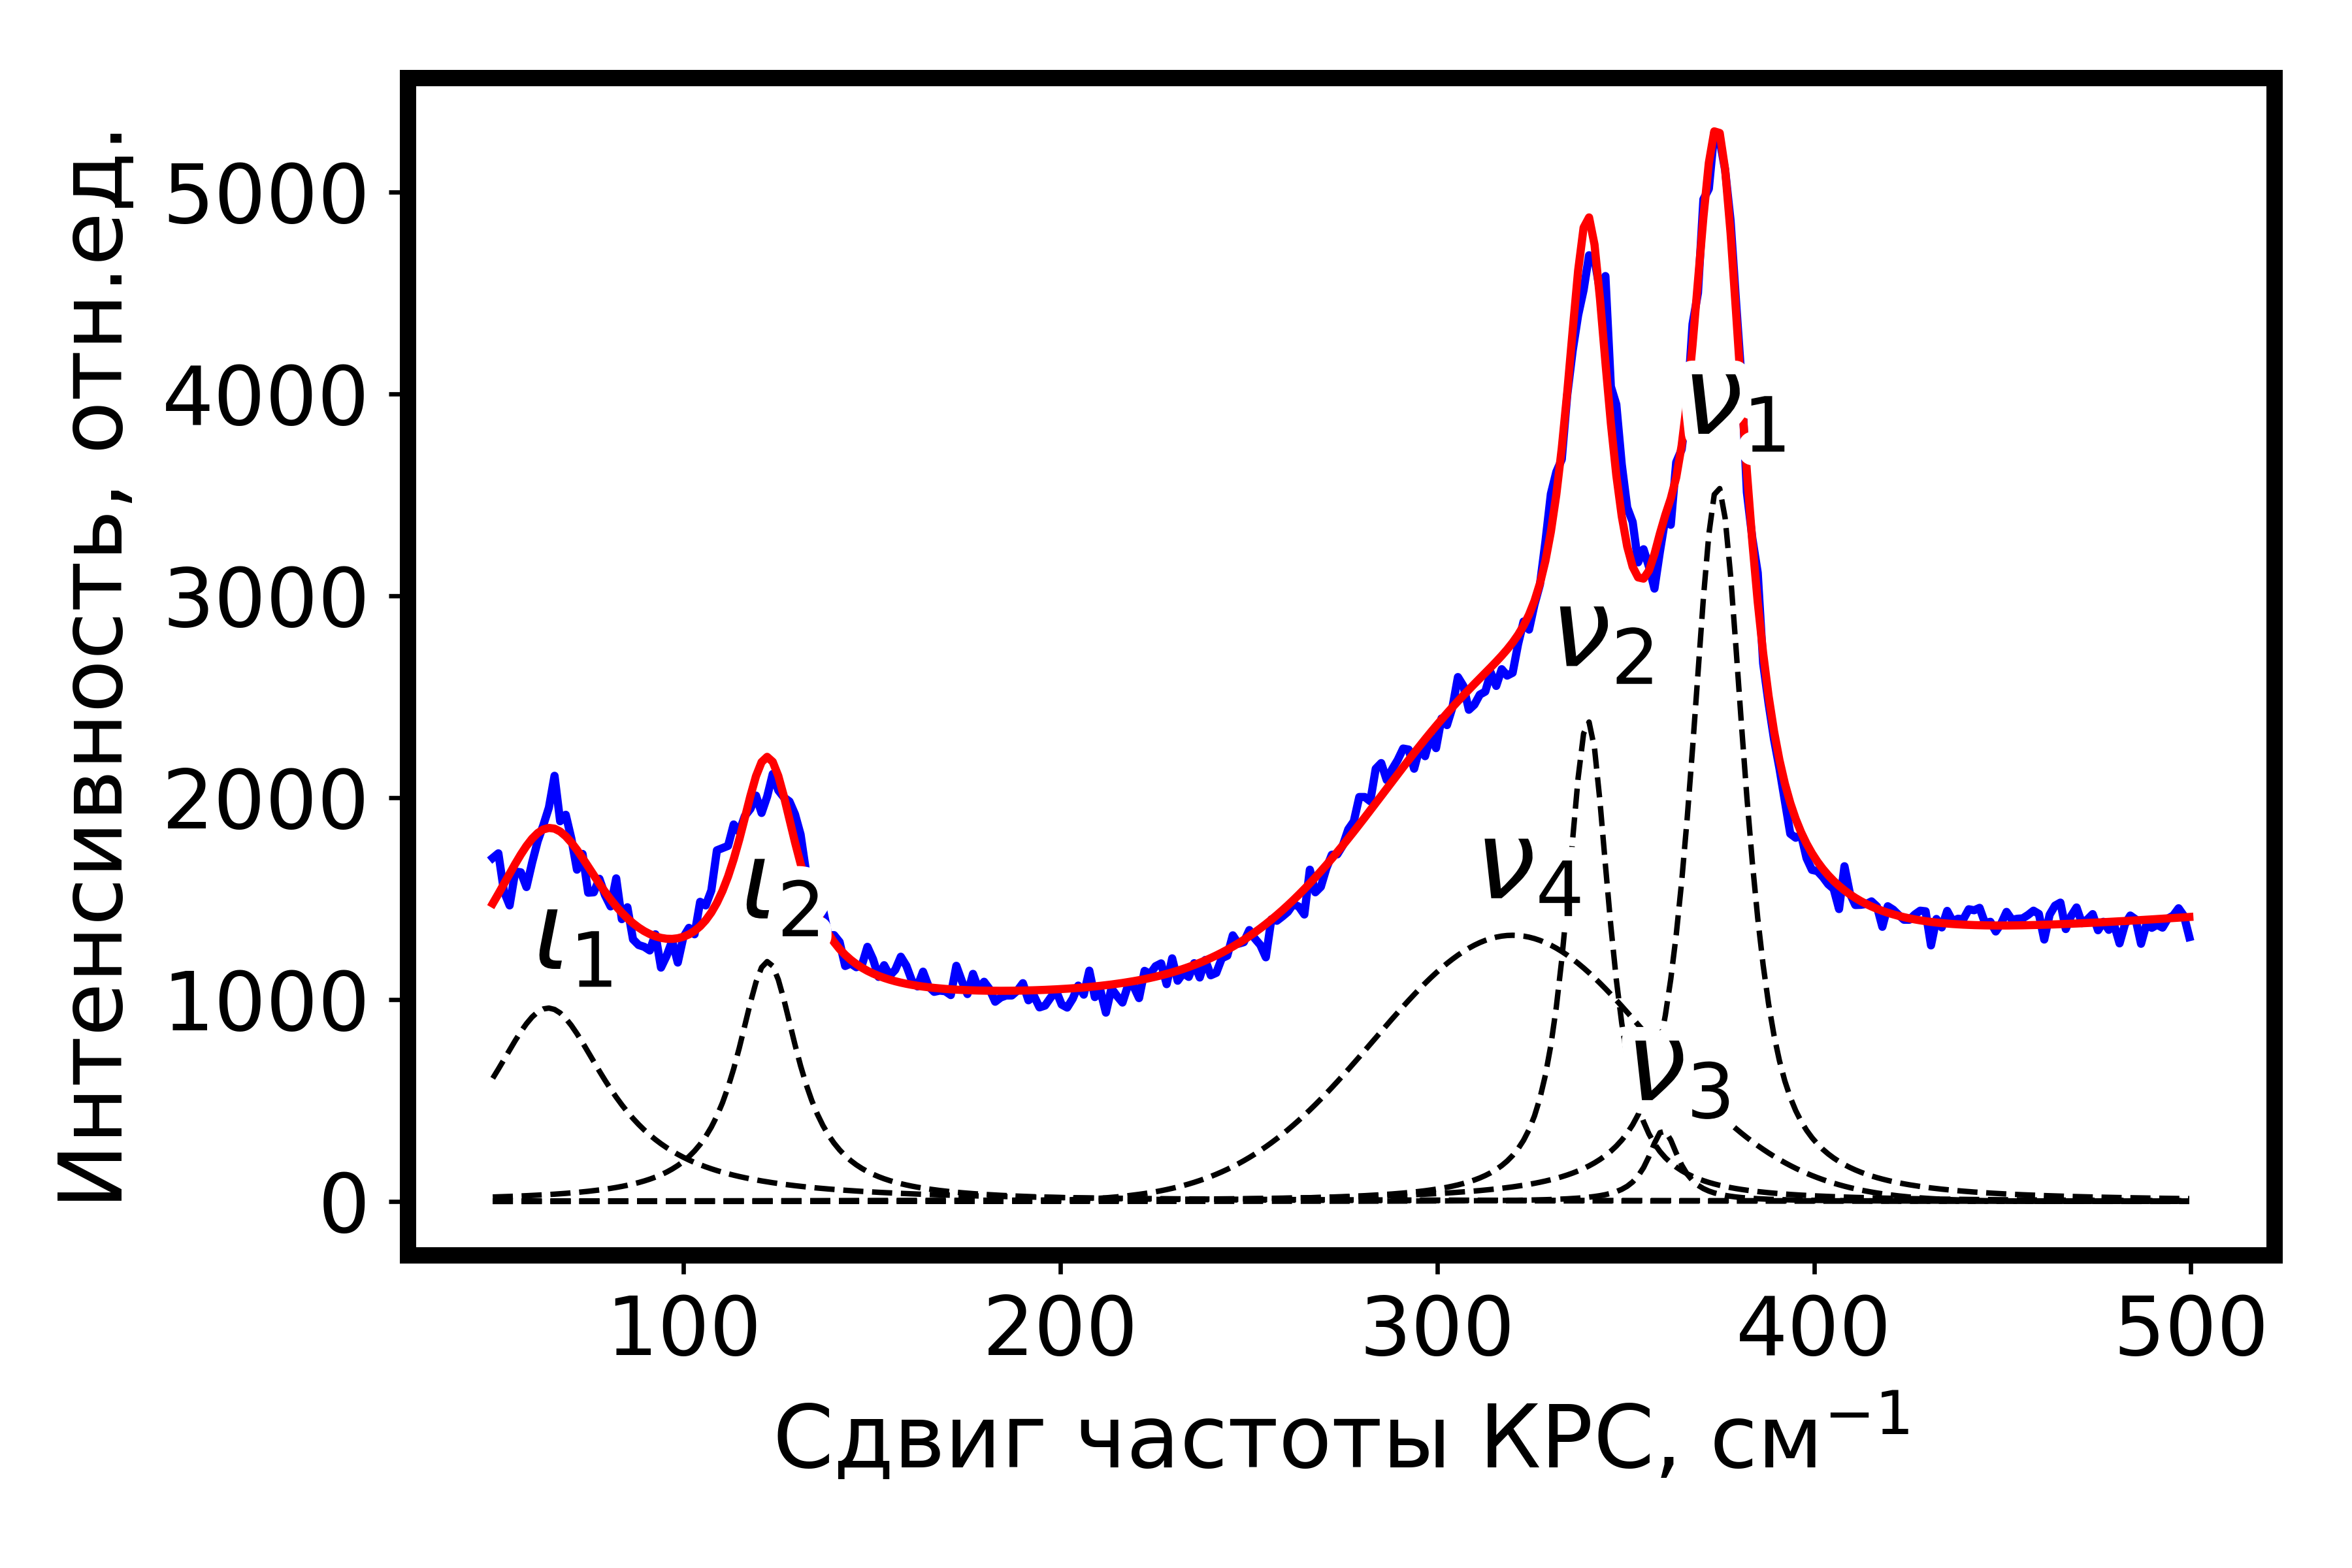
\includegraphics[width=0.9\linewidth]{raman_25_CuAsS3_rus_components}

      \caption[Спектр комбинационного рассеяния синтетического теннатита Cu\textsubscript{12}As\textsubscript{4}S\textsubscript{13}]{Спектр комбинационного рассеяния синтетического теннатита Cu\textsubscript{12}As\textsubscript{4}S\textsubscript{13}}

    \label{img:raman1a}
\end{figure}

\newpage


\section{Квантовомеханические расчёты структур синтетического теннантиа Cu\textsubscript{12}As\textsubscript{4}S\textsubscript{13}} \label{sect3_4}

Для исследования наиболее выгодного положения атомов меди были рассчитаны энергии 20 структур с разным положением атомов меди.
Структуры разделены на две группы: первая --- в лавесовском полиэдре сдвинуты 6 атомов меди (структуры с 1 по 10), вторая --- сдвинуты 3 атома меди в лавесовском полиэдре (структуры с 10 по 19). Изображения рассчитанных структур представлены на рисунках \ref{img:laves1}, \ref{img:laves2}, \ref{img:laves3} и \ref{img:laves4}.
На рисунке \ref{img:th} изображен график со значениями энергий элементарных ячеек для рассчитанных структур. Красной пунктирной линией обозначена энергия исходной структуры.
Экспериментальные структуры, полученные после анализа рентгеноструктурных экспериментов при разных температурах, были рассчитаны с учетом ферромагнитного, антиферромагнитного, парамагнитного (ПМ) и диамагнитного состояний в структурах.
Антиферромагнитное упорядочение в экспериментальной структуре при 85~К энергетически более выгодно, чем ферро- или пара- или диамагнитное состояния. При этом для 293~К ФМ, АФМ, ПМ конфигурации имеют одинаковую (до 4 знака) энергию, что указывает на их одинаковую выгодность и устойчивость.

\begin{figure}[ht!]
  \begin{minipage}[ht]{0.9\linewidth}\centering
    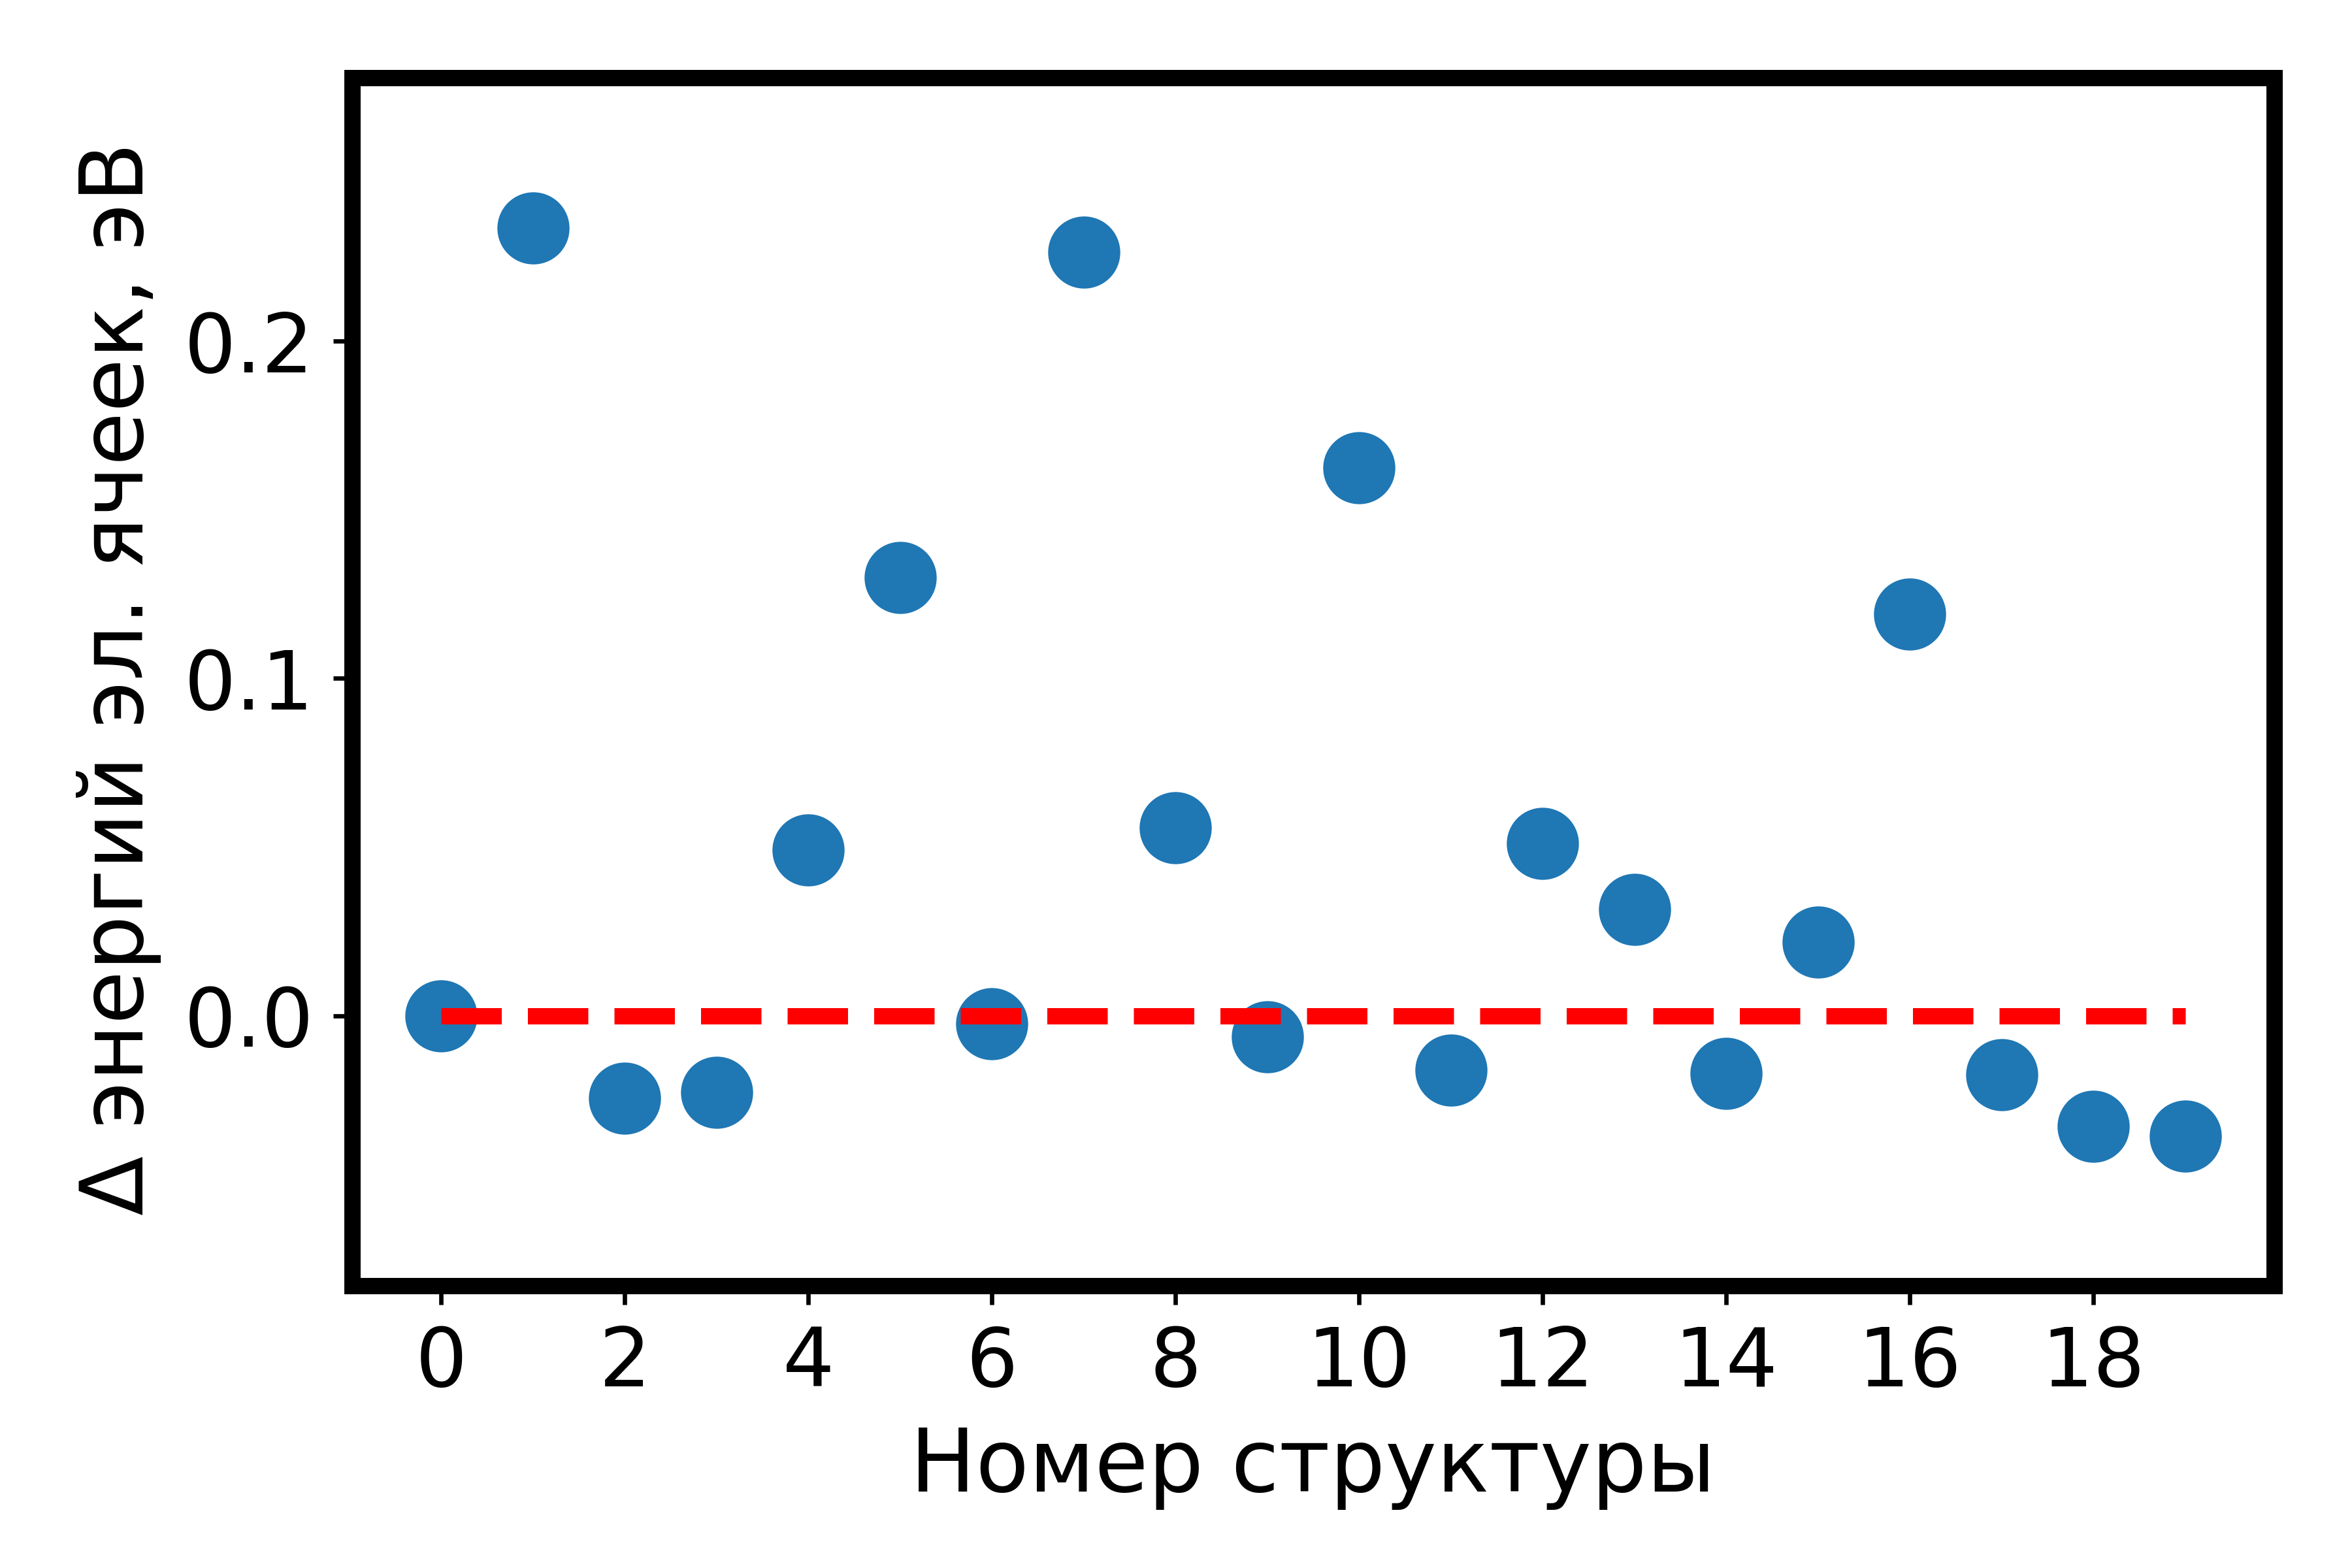
\includegraphics[width=0.7\linewidth]{energy_structure}
  \end{minipage}

      \caption[Сводный график энергий рассчитанных структур относительно энергии исходной структуры с разным расположением атомов в лавесовском полиэдре]{Сводный график энергий рассчитанных структур относительно энергии исходной структуры с разным расположением атомов в лавесовском полиэдре}
    \label{img:th}
\end{figure}

\begin{landscape}
\begin{table} [htbp]
\centering

\caption{Сводная таблица распределения электрических зарядов для рассчитанных структур (варианты с 0 по 9 включительно) с разным расположением атомов меди в лавесовском полиэдре для синтетического теннантита Cu\textsubscript{12}As\textsubscript{4}S\textsubscript{13}}%
	\label{mod_char1}% label всегда желательно идти после caption
    \renewcommand{\arraystretch}{1.5}
	%\resizebox{\textwidth}{!}{
    \begin{tabular}{@{}@{\extracolsep{10pt}}lllllllllll@{}}
      \toprule     %%% верхняя линейка
Atom & Var0          & Var1          & Var2          & Var3          & Var4   & Var5          & Var6          & Var7          & Var8          & Var9              \\  \midrule
Cu1                  & +0.57	                & +0.56	                  & {\bf +0.56 }	& {\bf +0.56 }	& +0.56	& +0.56	                  & +0.56	& +0.56	& +0.56	                  & {\bf +0.56} \\
\multirow{2}{*}{Cu2} & \multirow{2}{*}{+0.49}	& \multirow{2}{*}{+0.47}	& {\bf +0.45 }	& {\bf +0.49 }	& +0.47 & +0.51	                  & +0.49	& +0.49	& +0.49	                  & {\bf +0.50} \\
		                 &		                    &                         & {\bf +0.40 }	& {\bf +0.39 }	& +0.40	& +0.47	                  & +0.39	& +0.39	& +0.45	                  & {\bf +0.46} \\
\multirow{2}{*}{S1}  & -1.41	                & -1.45	                  & {\bf -1.42 }  & {\bf -1.42 }	& -1.39	& \textcolor{red}{-0.76}	& -1.43	& -1.43	& \textcolor{blue}{-0.73}	& \textcolor{blue}{-0.70} \\
                     & -1.47	                & -1.53	                  & {\bf -1.49 }  & {\bf -1.50 }	& -1.47	& \textcolor{red}{-0.92}	& -1.53	& -1.52	& \textcolor{blue}{-1.42}	& \textcolor{blue}{-1.44} \\
S2                   & -0.88	                & -0.85	                  & {\bf -0.78 }  & {\bf -0.82 }	& -0.84	& -0.84	                  & -0.83	& -0.83	& -0.86	                  & {\bf -0.86} \\
\multirow{2}{*}{As}  & \multirow{2}{*}{+2.97}	& +3.05	                  & {\bf +3.12 }	& {\bf +3.15 }	& +3.06	& +0.86	                  & +3.11	& +3.12	& \textcolor{blue}{+2.03}	& \textcolor{blue}{+1.51} \\
	                   &                        & +2.99	                  & {\bf +2.99 }  & {\bf +3.07 }	& +3.11	& +0.93	                  & +3.06	& +3.07	& \textcolor{blue}{+1.53}	& \textcolor{blue}{+0.89} \\
\bottomrule

\end{tabular}
%}
\end{table}
\end{landscape}

\begin{landscape}
\begin{table} [htbp]
\centering
\caption{Сводная таблица распределения электрических зарядов для рассчитанных структур (варианты с 10 по 19 включительно) с разным расположением атомов меди в лавесовском полиэдре для синтетического теннантита Cu\textsubscript{12}As\textsubscript{4}S\textsubscript{13}}%
	\label{mod_char2}% label всегда желательно идти после caption
    \renewcommand{\arraystretch}{1.5}
	\begin{tabular}{@{}@{\extracolsep{10pt}}lllllllllll@{}}

\toprule     %%% верхняя линейка
Atom                         &Var10& Var11& Var12& Var13 & Var14& Var15& Var16& Var17& Var18& Var19          \\ \hline
Cu1                  & +0.56   & 	{\bf +0.56 }           & 	+0.56  & 	+0.56                  & 	{\bf +0.56 }           & 	+0.56                  & 	+0.56                  & 	{\bf +0.56 }           & 	{\bf +0.56 }           & 	{\bf +0.56 } \\
\multirow{2}{*}{Cu2} & +0.48   & 	{\bf +0.51 }           & 	+0.46  & 	+0.51                  & 	{\bf +0.50 }           & 	+0.51                  & 	+0.51                  & 	{\bf +0.51 }           & 	{\bf +0.51 }           & 	{\bf +0.50 } \\
		                 & +0.39   & 	{\bf +0.48 }           & 	+0.45  & 	+0.47                  & 	{\bf +0.46 }           & 	+0.46                  & 	+0.45                  & {\bf +0.46 }            & 	{\bf +0.46 }           & 	{\bf +0.46 } \\
\multirow{2}{*}{S1}  & -1.43   & 	\textcolor{red}{-0.73} & 	-1.42  & 	\textcolor{red}{-0.72} & 	\textcolor{red}{-0.73} & 	\textcolor{red}{-0.73} & 	\textcolor{red}{-0.72} & 	\textcolor{red}{-0.72} & 	\textcolor{red}{-0.74} & 	\textcolor{red}{-0.72} \\
                     & -1.52   & 	\textcolor{red}{-0.76} & 	-1.52  & 	\textcolor{red}{-0.77} & 	\textcolor{red}{-0.76} & 	\textcolor{red}{-0.77} & 	\textcolor{red}{-0.77} & 	\textcolor{red}{-0.77} & 	\textcolor{red}{-0.76} & 	\textcolor{red}{-0.76} \\
S2                   & -0.82   & 	{\bf -0.98}            & 	-0.81  & 	-0.93                  & 	{\bf -0.90 }           & 	-0.94                  & 	-0.90                  & 	{\bf -0.88 }           & 	{\bf -0.91 }           & 	{\bf -0.89 } \\
\multirow{2}{*}{As}  & +3.11   & 	\textcolor{red}{+0.94} & 	+3.07  & \textcolor{red}{+0.94}  & 	\textcolor{red}{+0.94} & 	\textcolor{red}{+0.94} & 	\textcolor{red}{+0.95} & 	\textcolor{red}{+0.95} & 	\textcolor{red}{+0.91} & 	\textcolor{red}{+0.91} \\
	                   & +3.00	 & \textcolor{red}{+0.76}	 & +2.99	 & \textcolor{red}{+0.85}	 & \textcolor{red}{+0.80}	 & \textcolor{red}{+0.84}	 & \textcolor{red}{+0.87}	 & \textcolor{red}{+0.85}	 & \textcolor{red}{+0.85}	 & \textcolor{red}{+0.84} \\
 \bottomrule


\end{tabular}
\end{table}
\end{landscape}

\begin{figure}[p!]
  \begin{minipage}[ht]{0.45\linewidth}\centering
    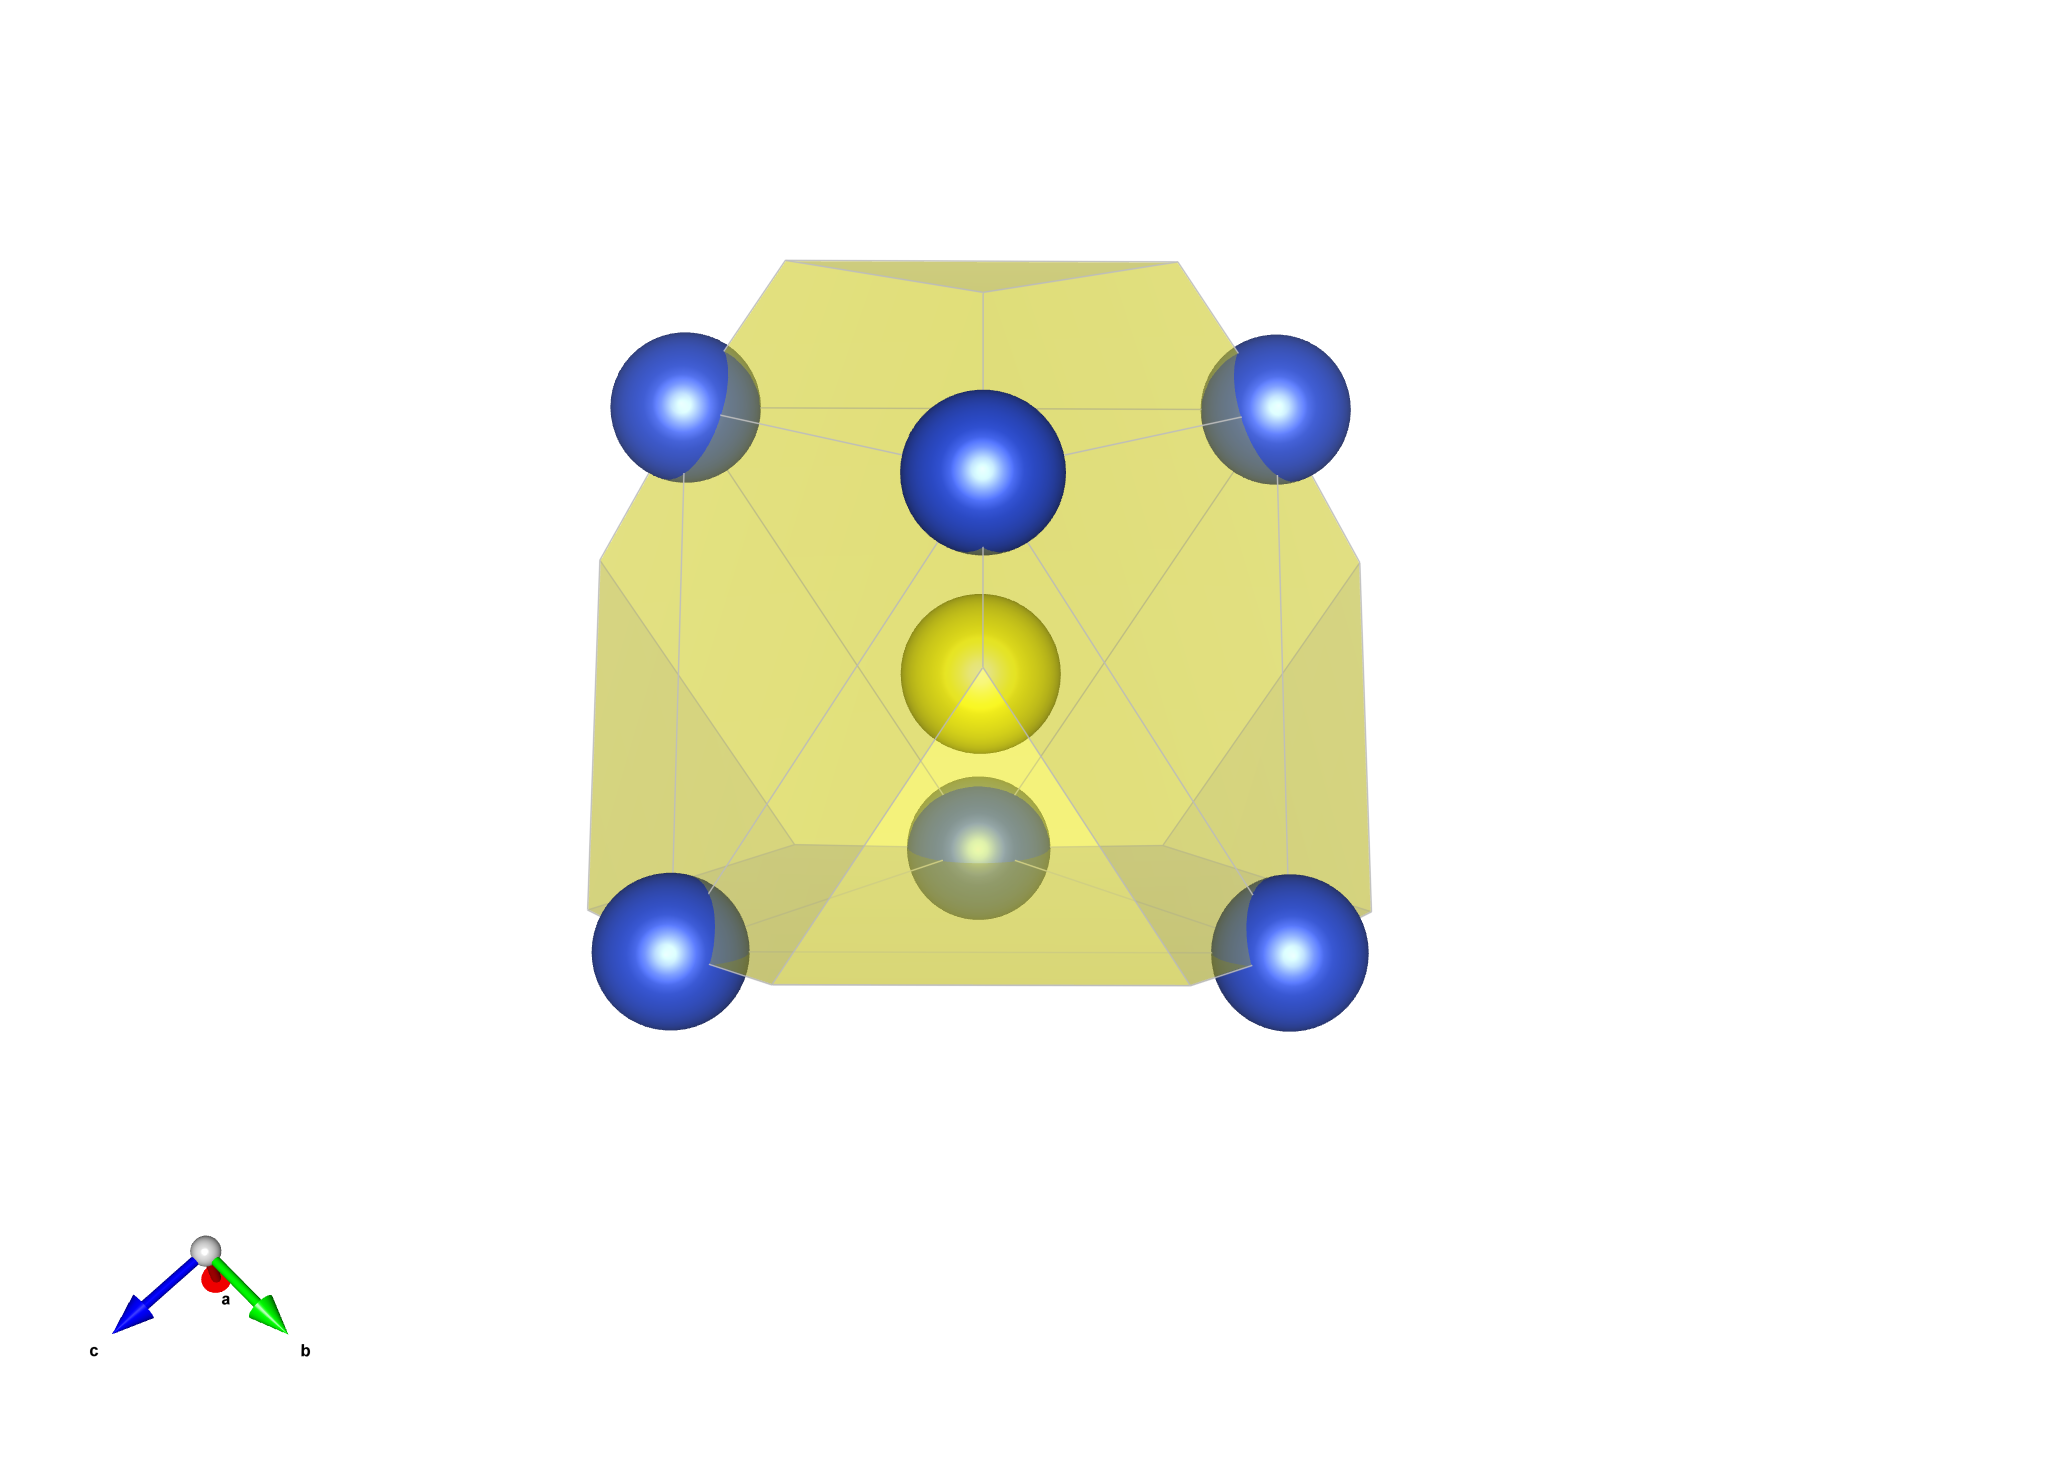
\includegraphics[width=0.9\linewidth]{var_0} \\ а)
  \end{minipage}
						\hfill
 \begin{minipage}[ht]{0.45\linewidth}\centering
    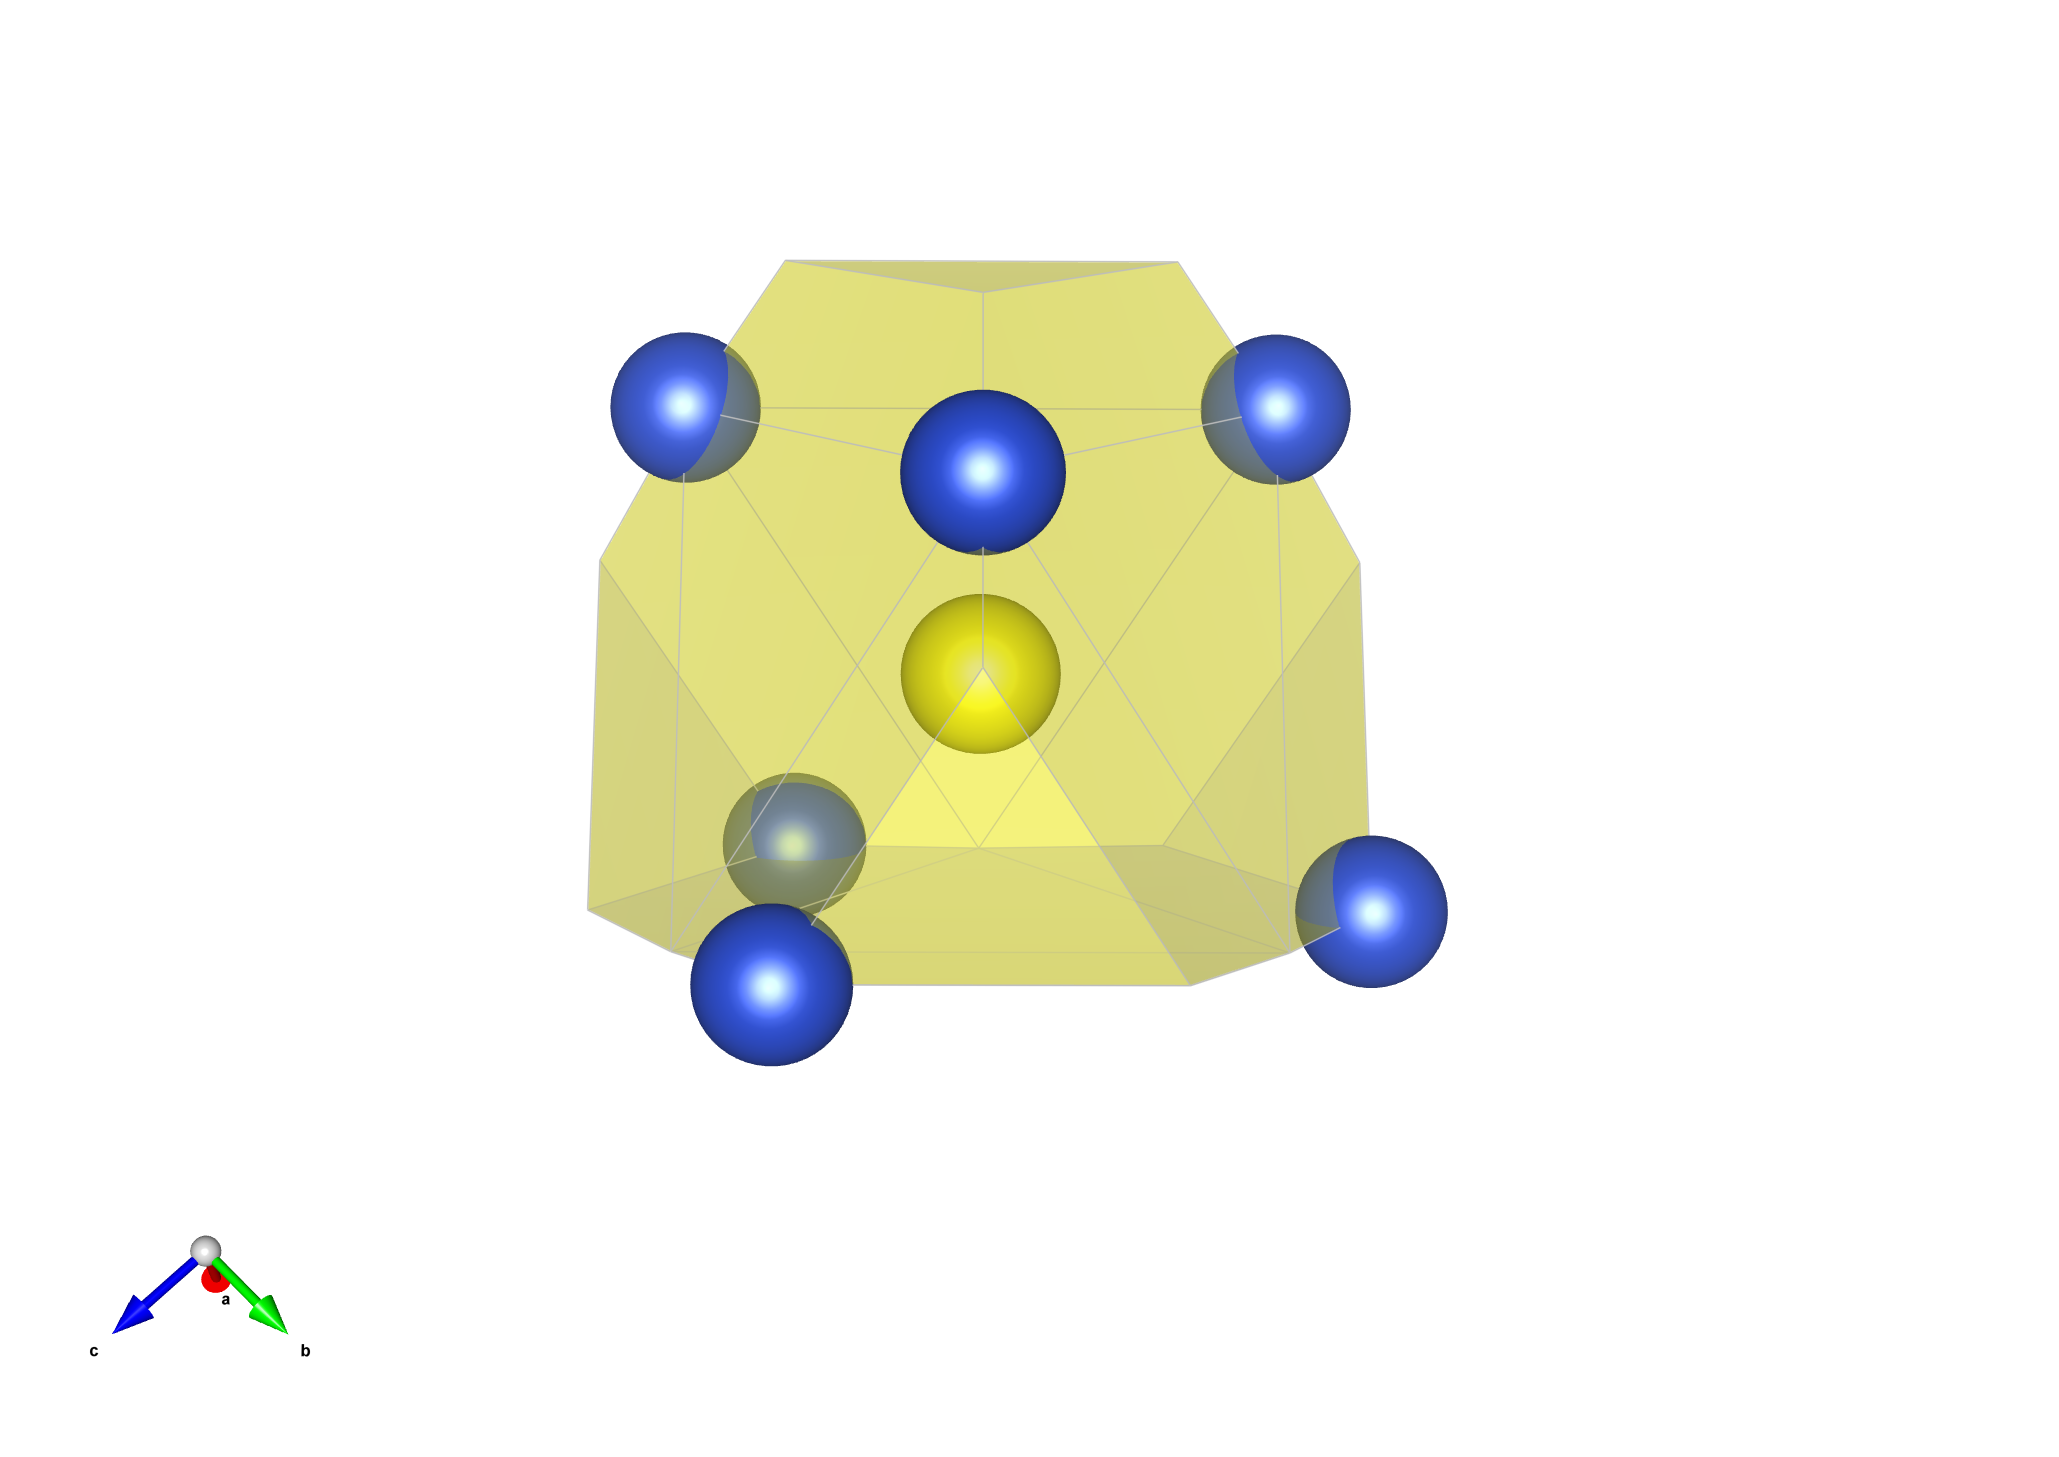
\includegraphics[width=0.9\linewidth]{var_1} \\ б)
  \end{minipage}
\vfill

  \begin{minipage}[ht]{0.45\linewidth}\centering
    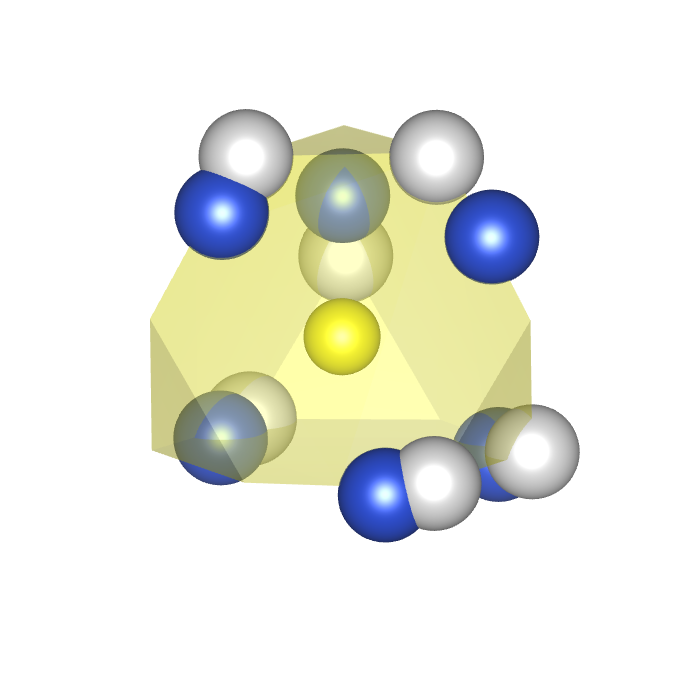
\includegraphics[width=0.9\linewidth]{var_2} \\ в)
  \end{minipage}
						\hfill
 \begin{minipage}[ht]{0.45\linewidth}\centering
    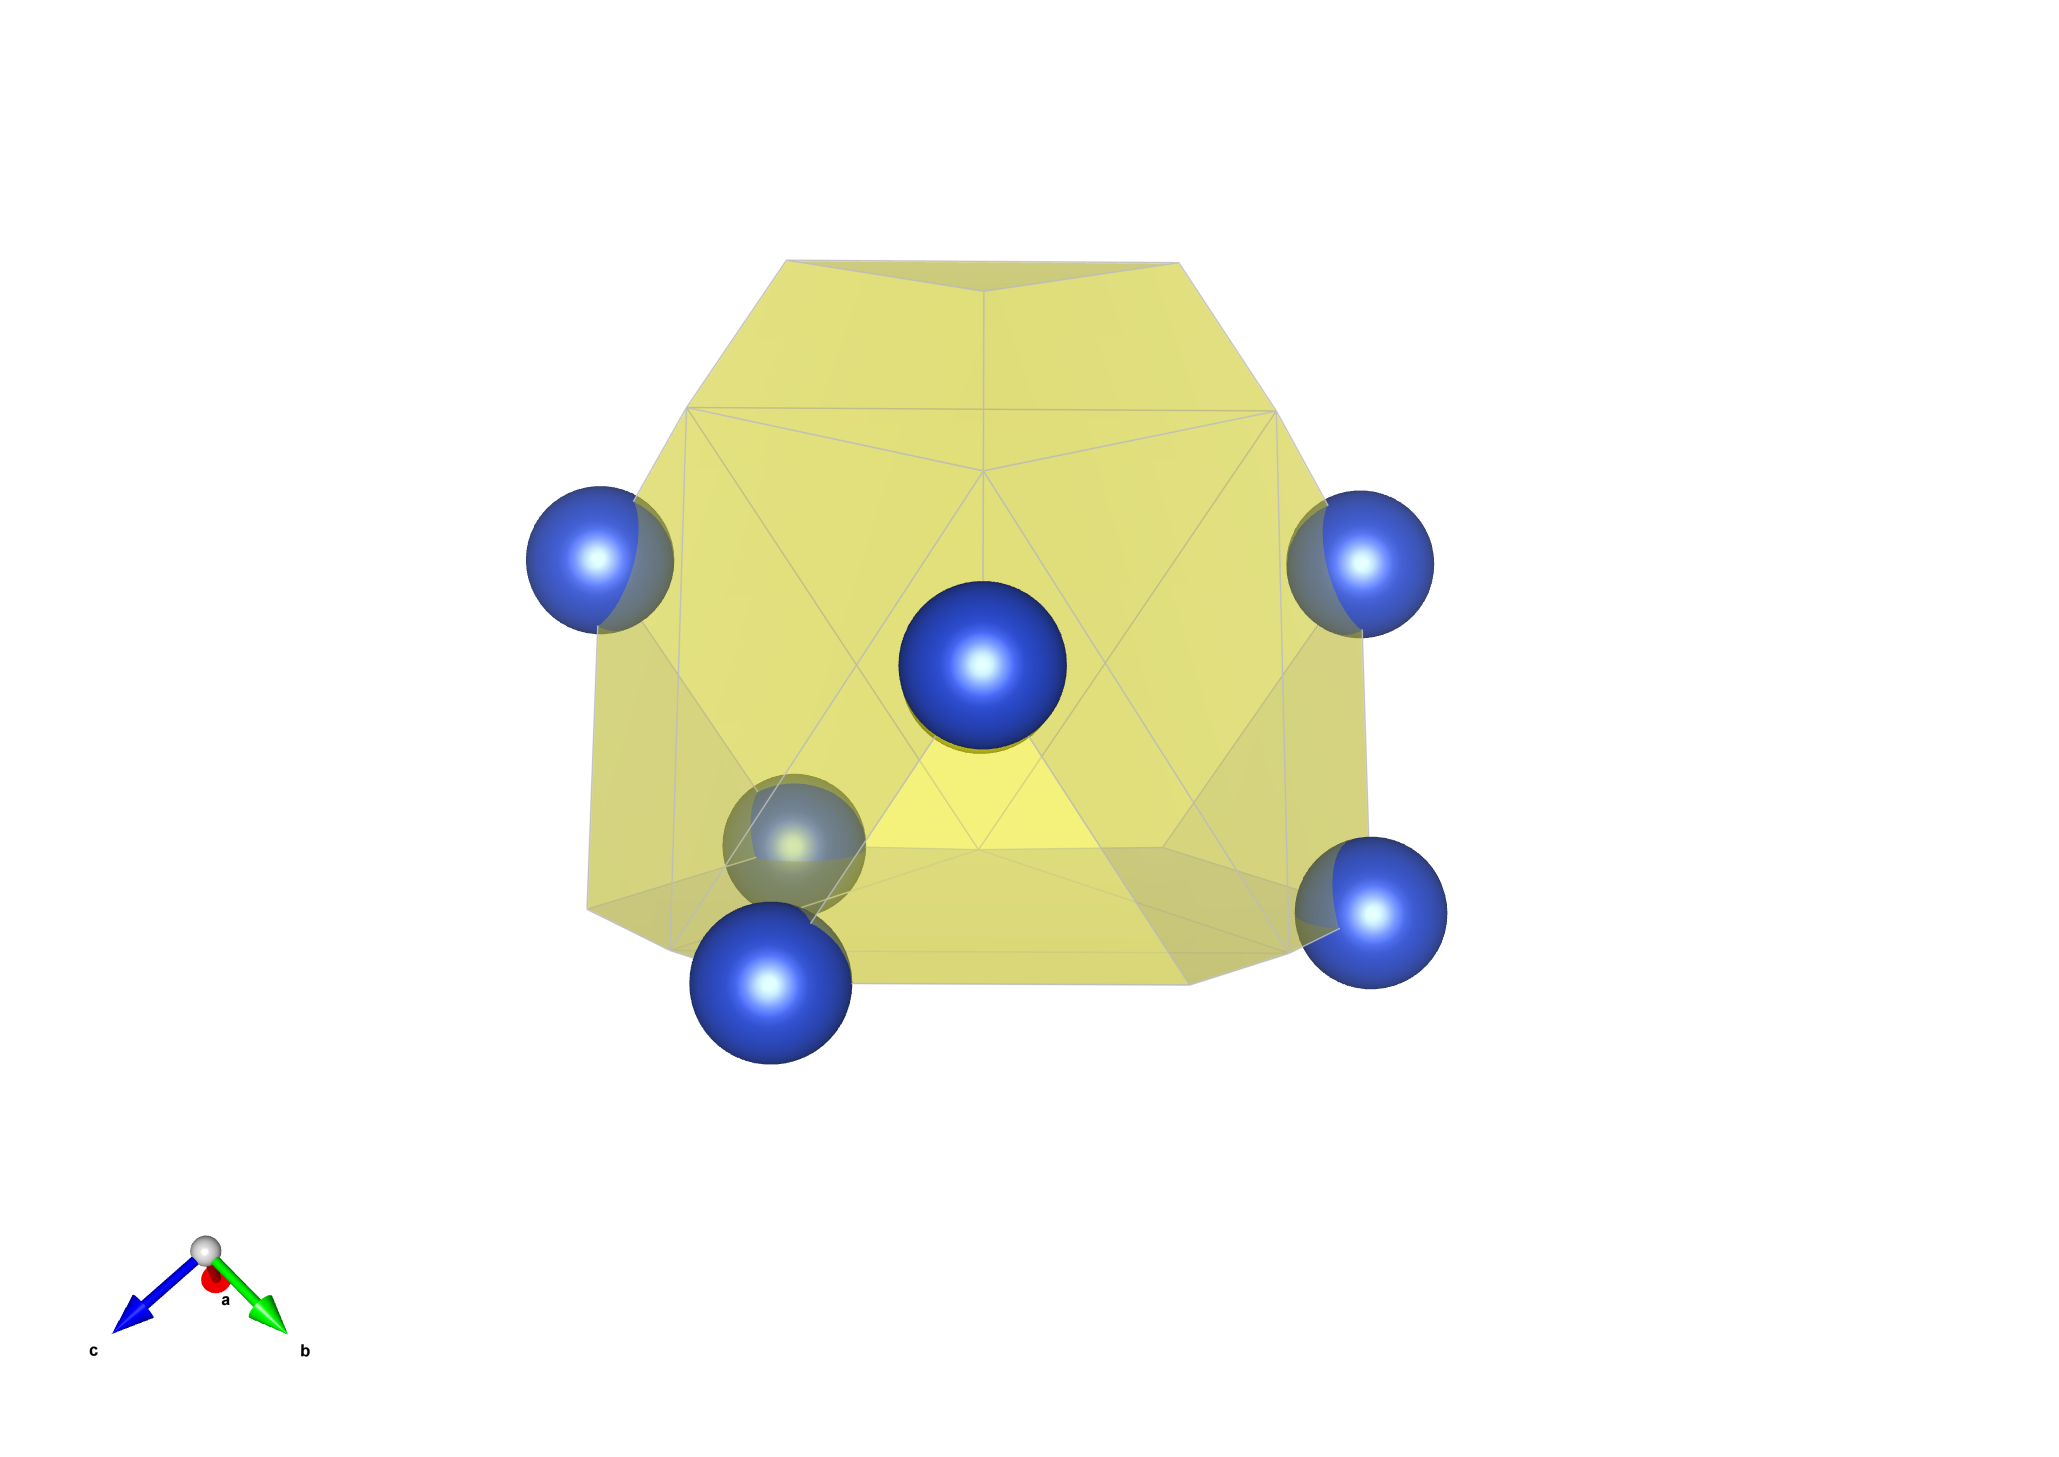
\includegraphics[width=0.9\linewidth]{var_3} \\ г)
  \end{minipage}
\vfill

  \begin{minipage}[ht]{0.45\linewidth}\centering
    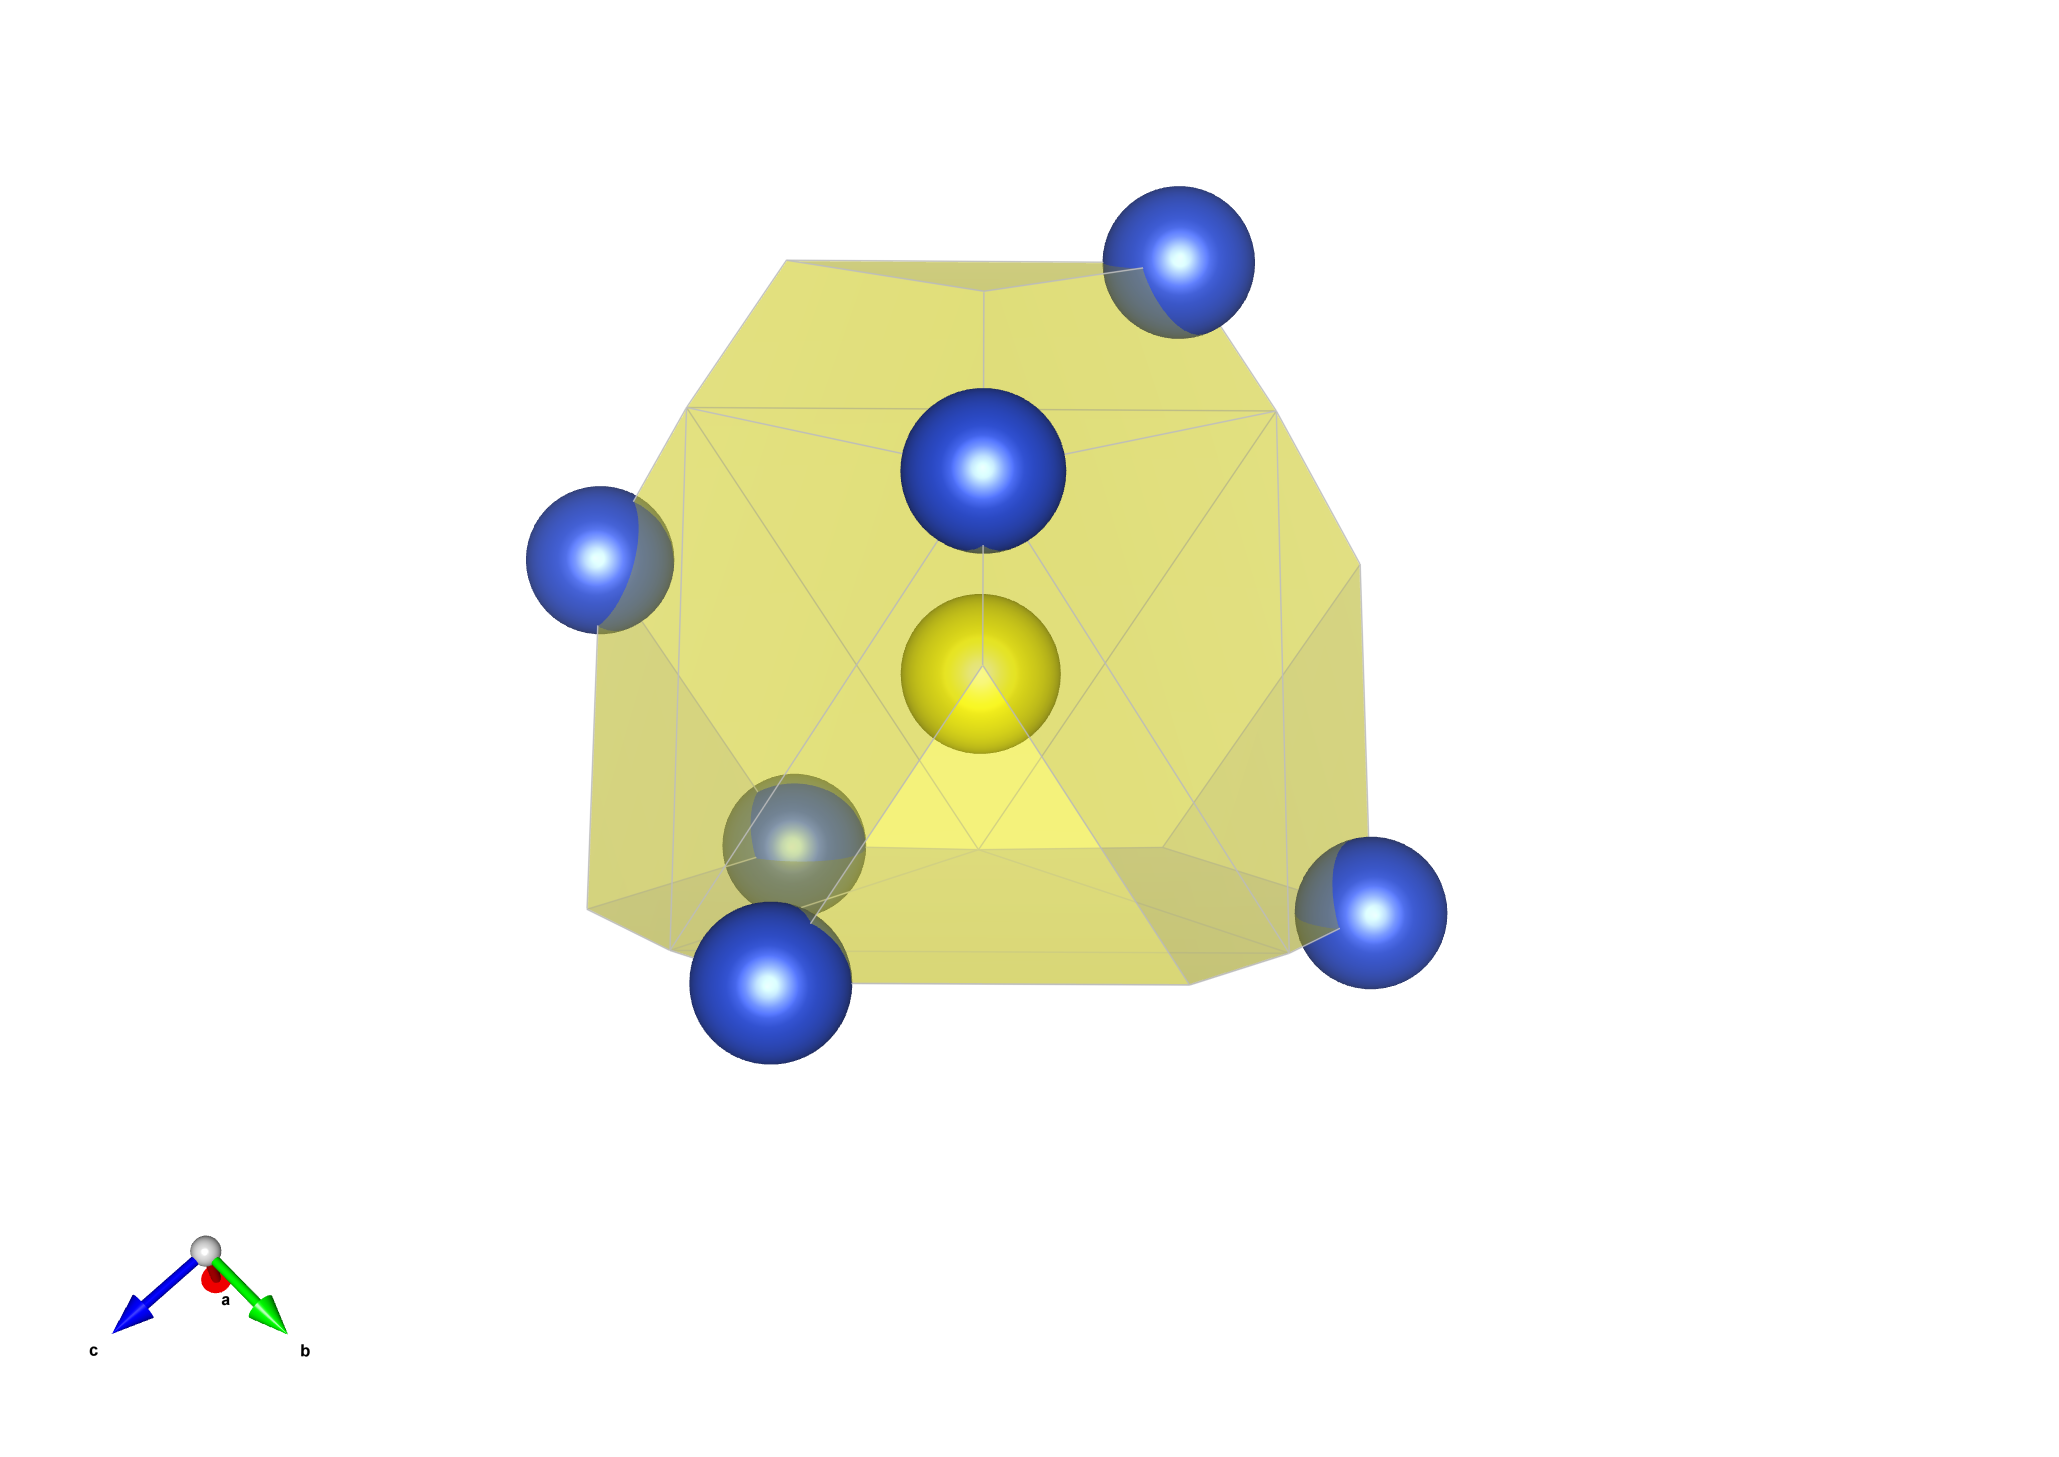
\includegraphics[width=0.9\linewidth]{var_4} \\ д)
  \end{minipage}
						\hfill
 \begin{minipage}[ht]{0.45\linewidth}\centering
    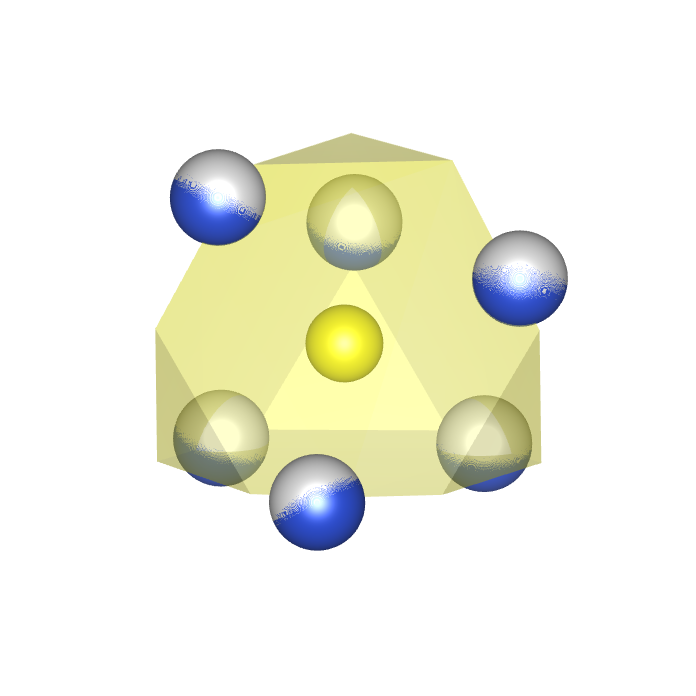
\includegraphics[width=0.9\linewidth]{var_5} \\ е)
  \end{minipage}
      \caption[Изображения лавесовских полиэдров синтетического теннантита Cu\textsubscript{12}As\textsubscript{4}S\textsubscript{13}, для которых рассчитывалась энергия элементарной ячейки. Варианты с 0 по 5 включительно]{Изображения лавесовских полиэдров синтетического теннантита Cu\textsubscript{12}As\textsubscript{4}S\textsubscript{13}, для которых рассчитывалась энергия элементарной ячейки. Варианты с 0 по 5 включительно}
    \label{img:laves1}
\end{figure}

\begin{figure}[p!]
  \begin{minipage}[ht]{0.45\linewidth}\centering
    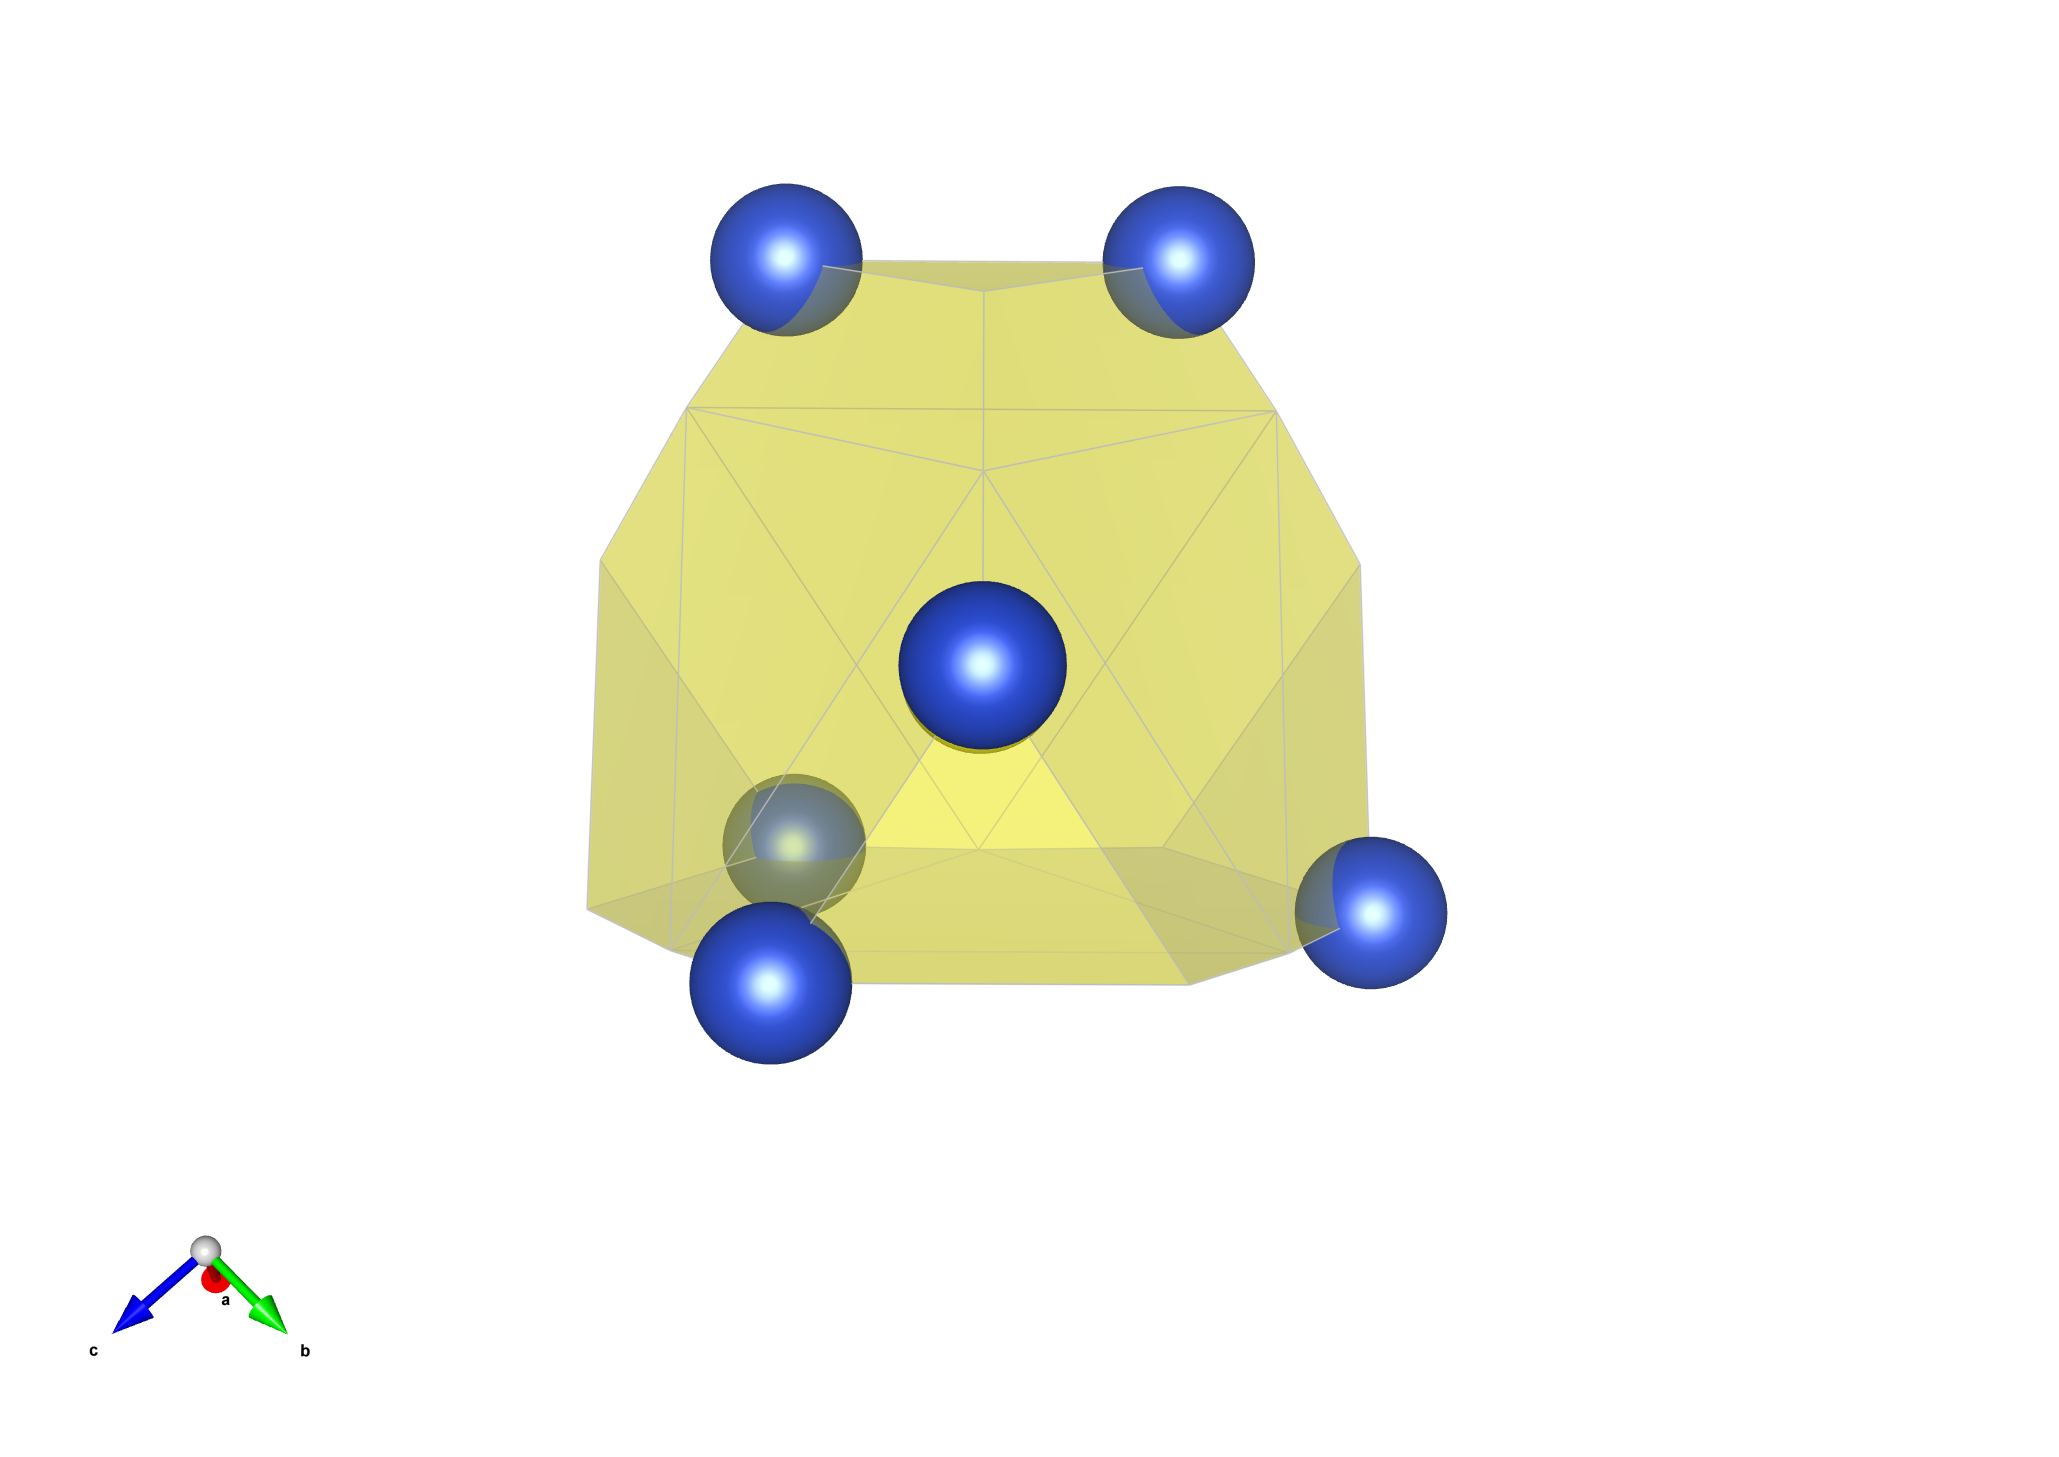
\includegraphics[width=0.9\linewidth]{var_6} \\ а)
  \end{minipage}
						\hfill
 \begin{minipage}[ht]{0.45\linewidth}\centering
    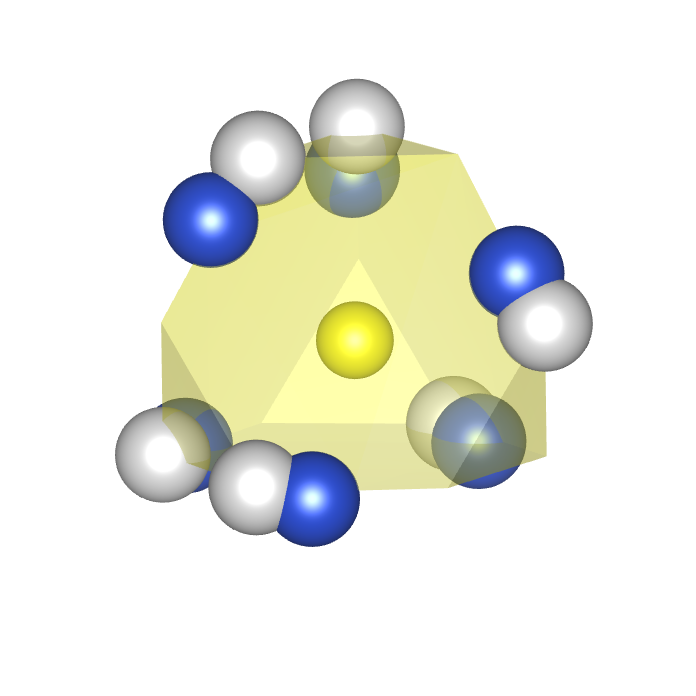
\includegraphics[width=0.9\linewidth]{var_7} \\ б)
  \end{minipage}
\vfill

  \begin{minipage}[ht]{0.45\linewidth}\centering
    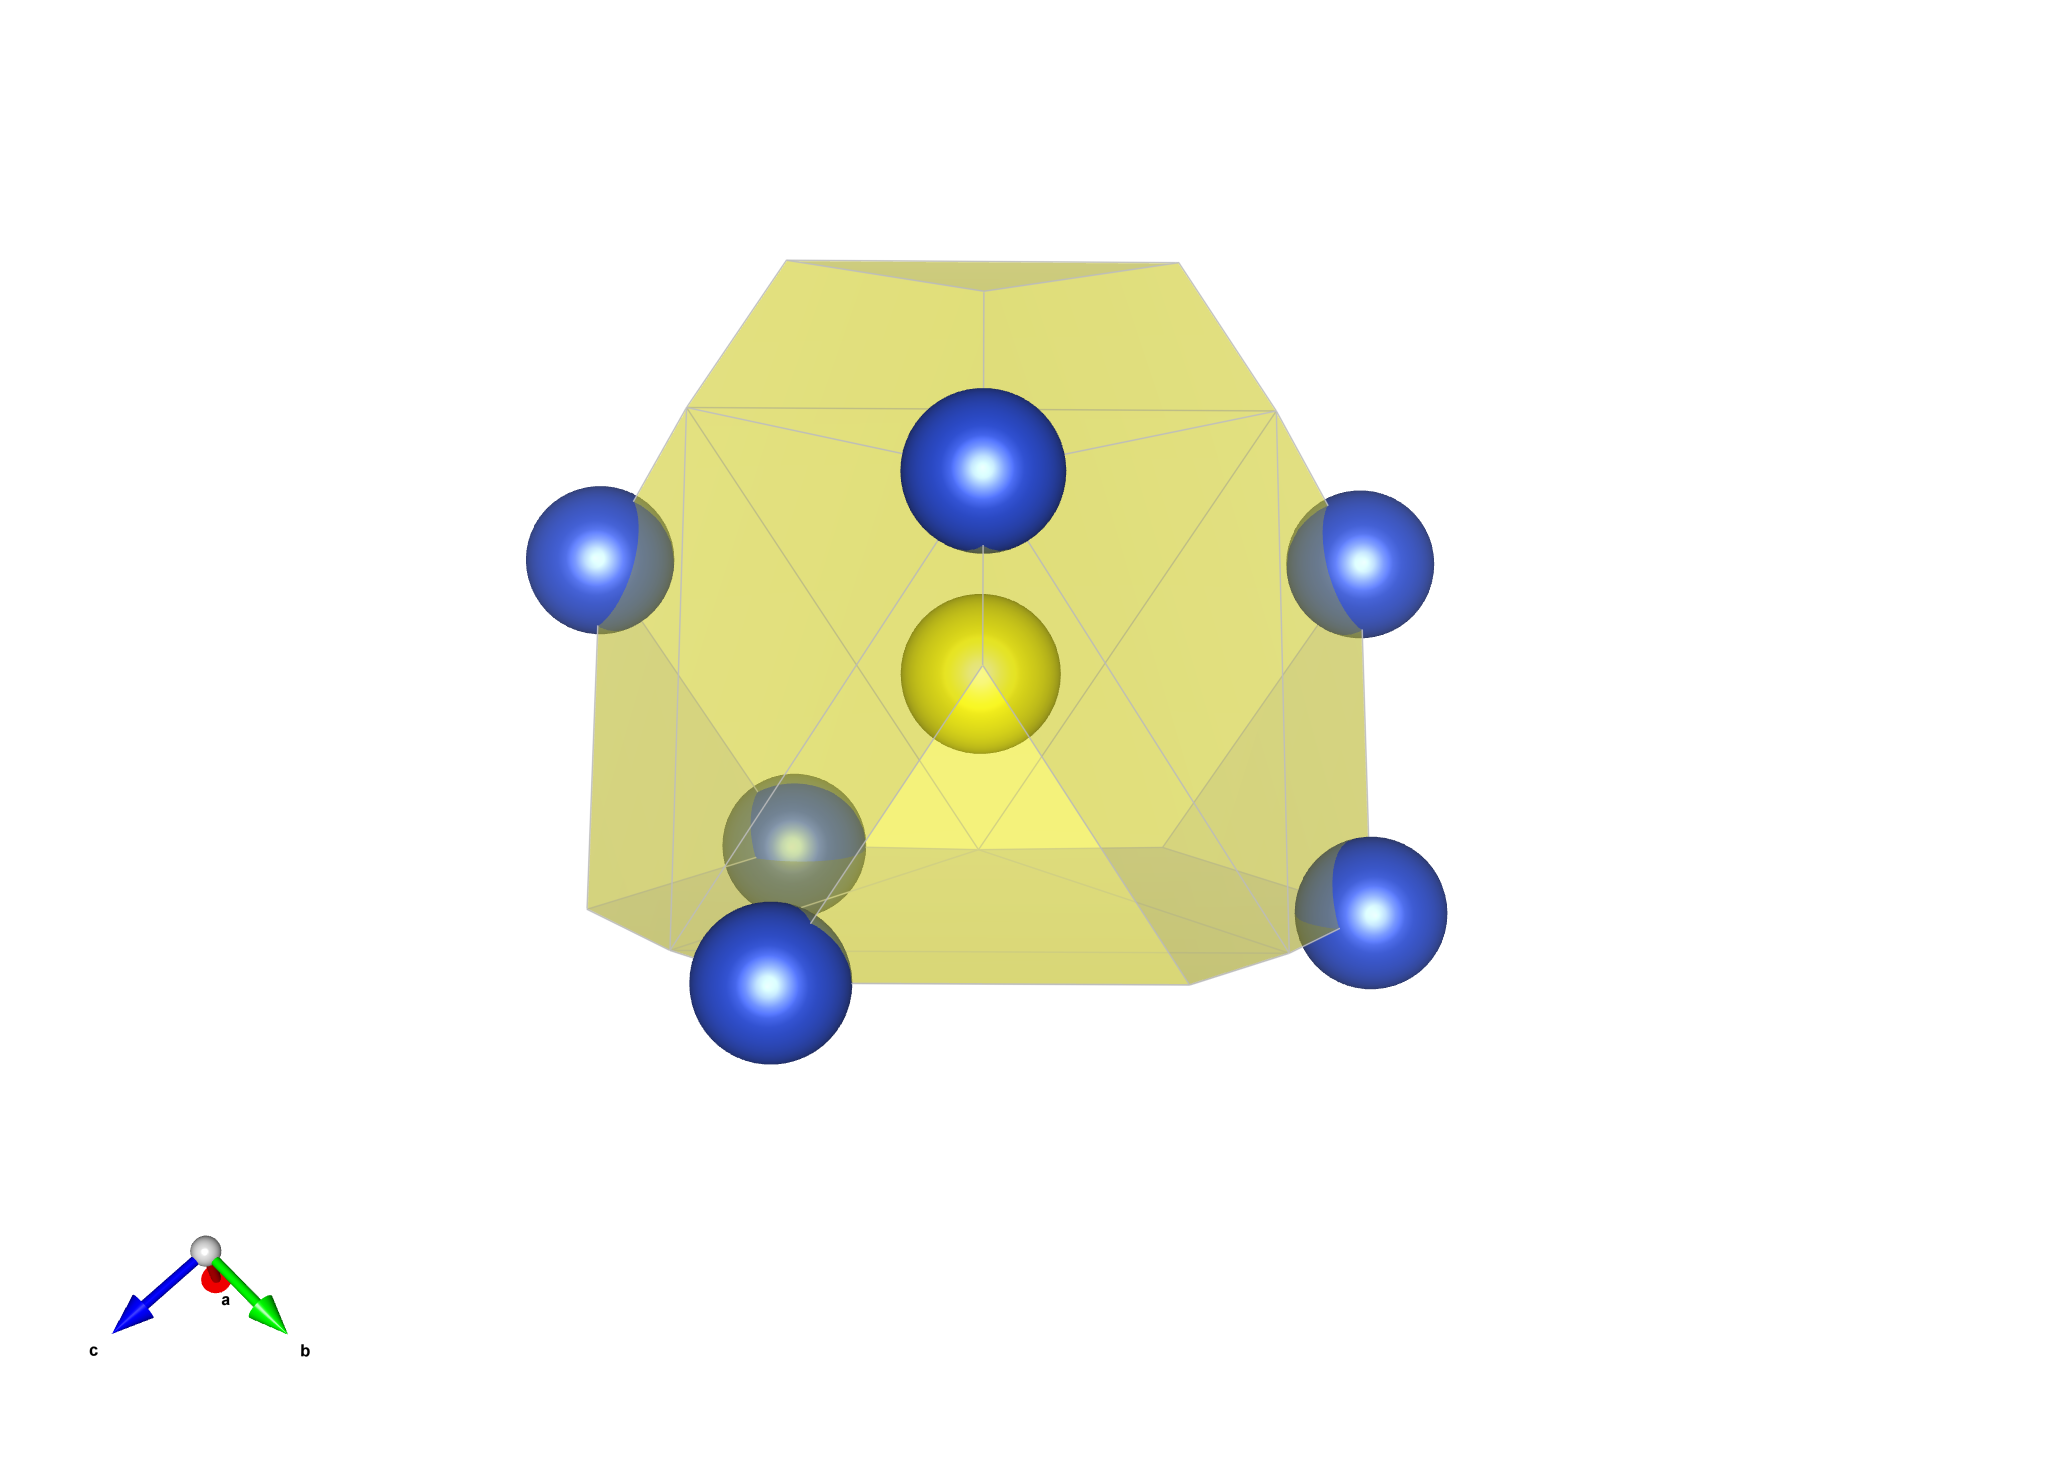
\includegraphics[width=0.9\linewidth]{var_8} \\ в)
  \end{minipage}
						\hfill
 \begin{minipage}[ht]{0.45\linewidth}\centering
    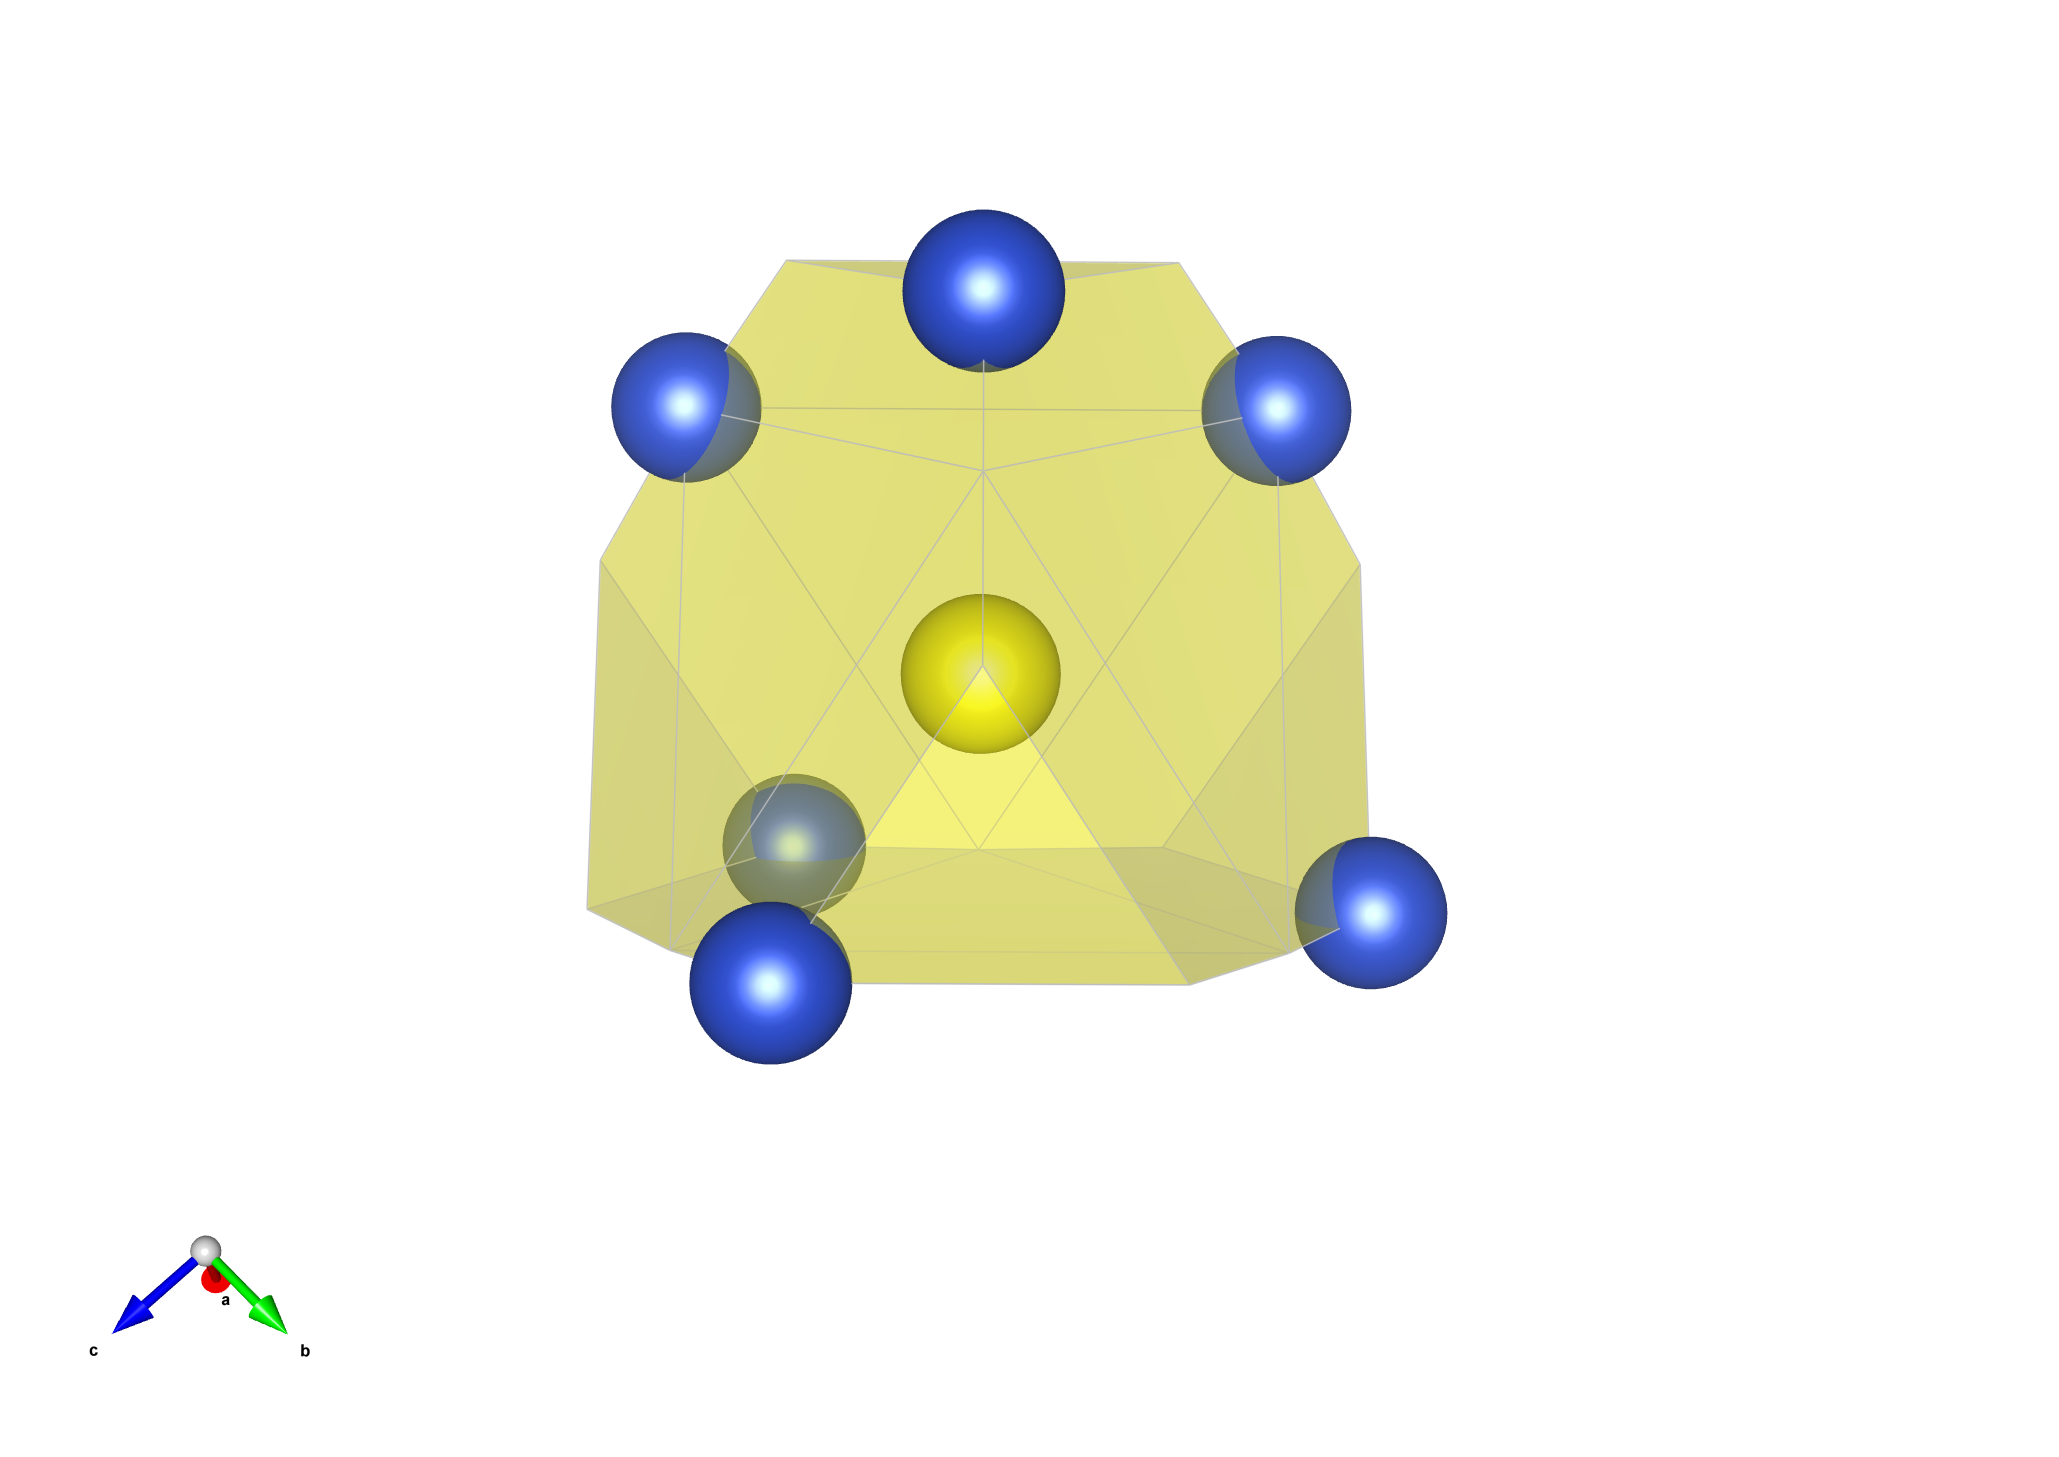
\includegraphics[width=0.9\linewidth]{var_9} \\ г)
  \end{minipage}
\vfill

  \begin{minipage}[ht]{0.45\linewidth}\centering
    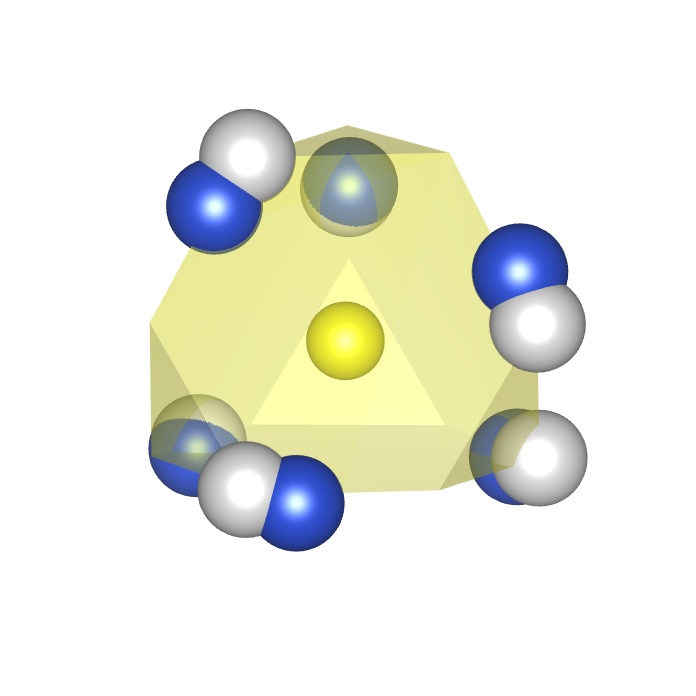
\includegraphics[width=0.9\linewidth]{var_10} \\ д)
  \end{minipage}
						\hfill
 \begin{minipage}[ht]{0.45\linewidth}\centering
    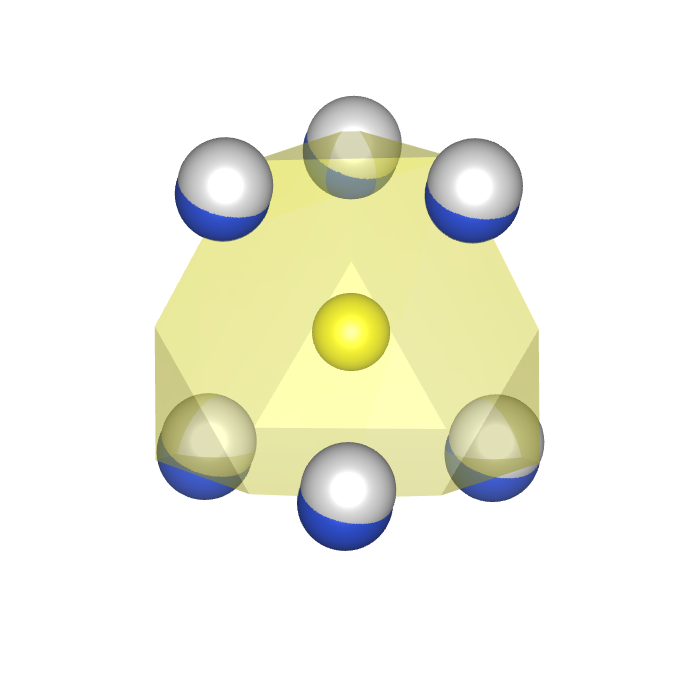
\includegraphics[width=0.9\linewidth]{var_11} \\ е)
  \end{minipage}
      \caption[Изображения лавесовских полиэдров синтетического теннантита Cu\textsubscript{12}As\textsubscript{4}S\textsubscript{13}, для которых рассчитывалась энергия элементарной ячейки. Варианты с 6 по 11 включительно]{Изображения лавесовских полиэдров синтетического теннантита Cu\textsubscript{12}As\textsubscript{4}S\textsubscript{13}, для которых рассчитывалась энергия элементарной ячейки. Варианты с 6 по 11 включительно}
    \label{img:laves2}
\end{figure}



\begin{figure}[p!]
  \begin{minipage}[ht]{0.45\linewidth}\centering
    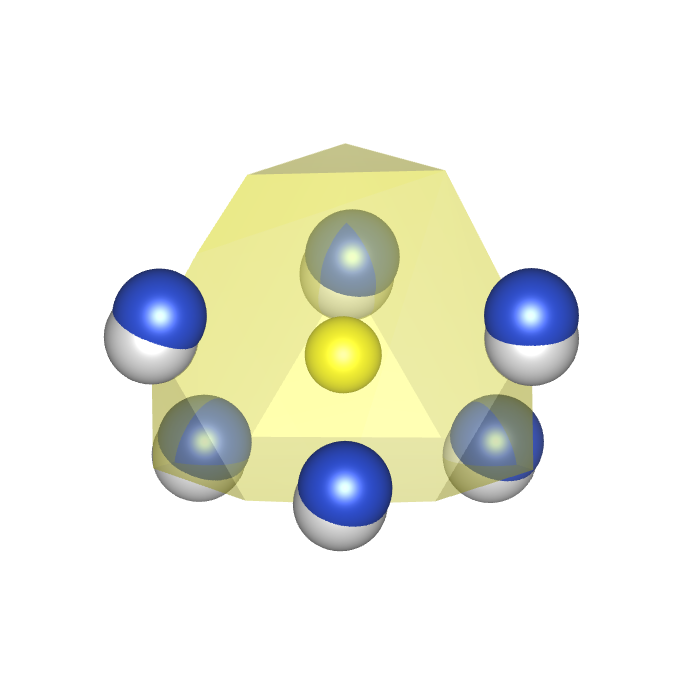
\includegraphics[width=0.9\linewidth]{var_12} \\ а)
  \end{minipage}
\hfill
 \begin{minipage}[ht]{0.45\linewidth}\centering
    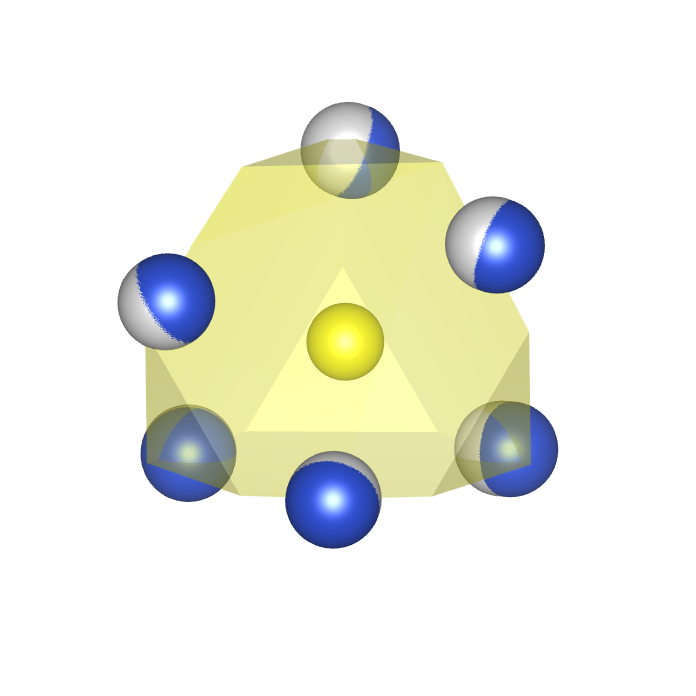
\includegraphics[width=0.9\linewidth]{var_13} \\ б)
  \end{minipage}
\vfill
  \begin{minipage}[ht]{0.45\linewidth}\centering
    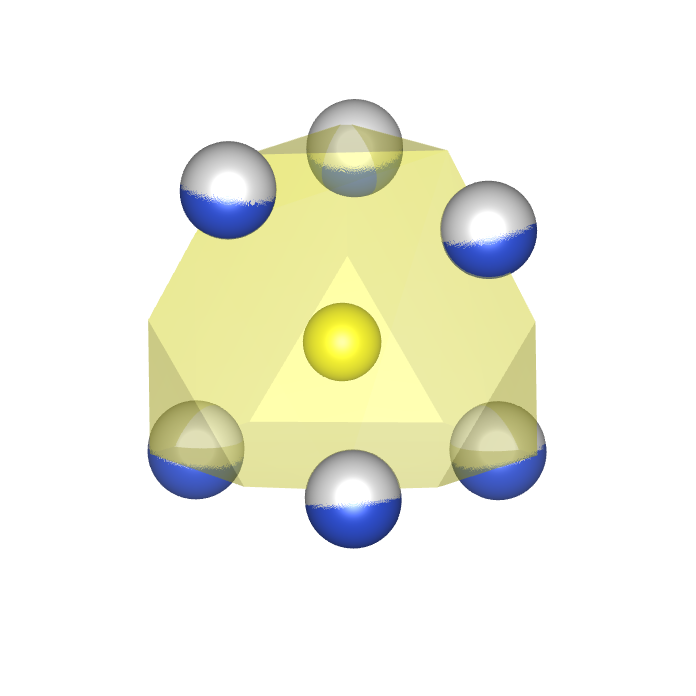
\includegraphics[width=0.9\linewidth]{var_14} \\ в)
  \end{minipage}
	\hfill
 \begin{minipage}[ht]{0.45\linewidth}\centering
    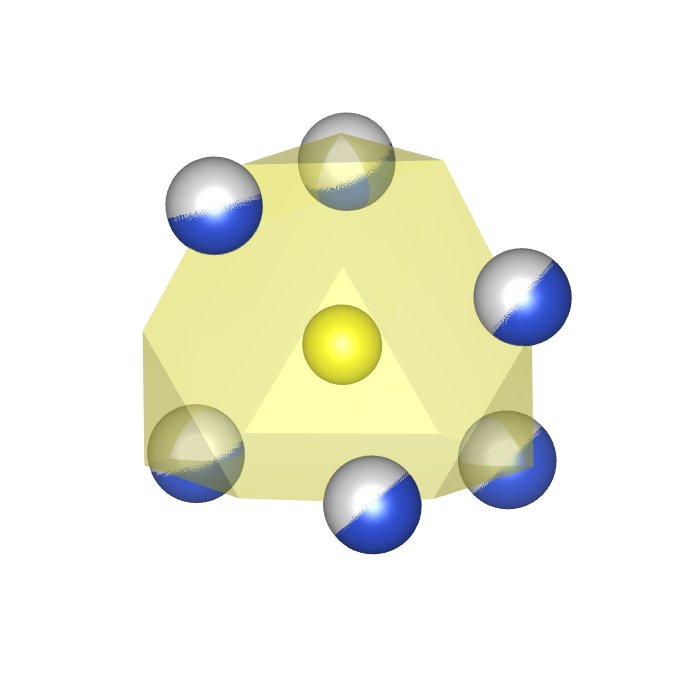
\includegraphics[width=0.9\linewidth]{var_15} \\ г)
  \end{minipage}
\vfill

  \begin{minipage}[ht]{0.45\linewidth}\centering

  \end{minipage}
						\hfill
 \begin{minipage}[ht]{0.45\linewidth}\centering

  \end{minipage}
      \caption[Изображения лавесовских полиэдров синтетического теннантита Cu\textsubscript{12}As\textsubscript{4}S\textsubscript{13}, для которых рассчитывалась энергия элементарной ячейки. Варианты с 12 по 15 включительно]{Изображения лавесовских полиэдров синтетического теннантита Cu\textsubscript{12}As\textsubscript{4}S\textsubscript{13}, для которых рассчитывалась энергия элементарной ячейки. Варианты с 12 по 15 включительно}
    \label{img:laves3}
\end{figure}


\begin{figure}[p!]
  \begin{minipage}[ht]{0.45\linewidth}\centering
    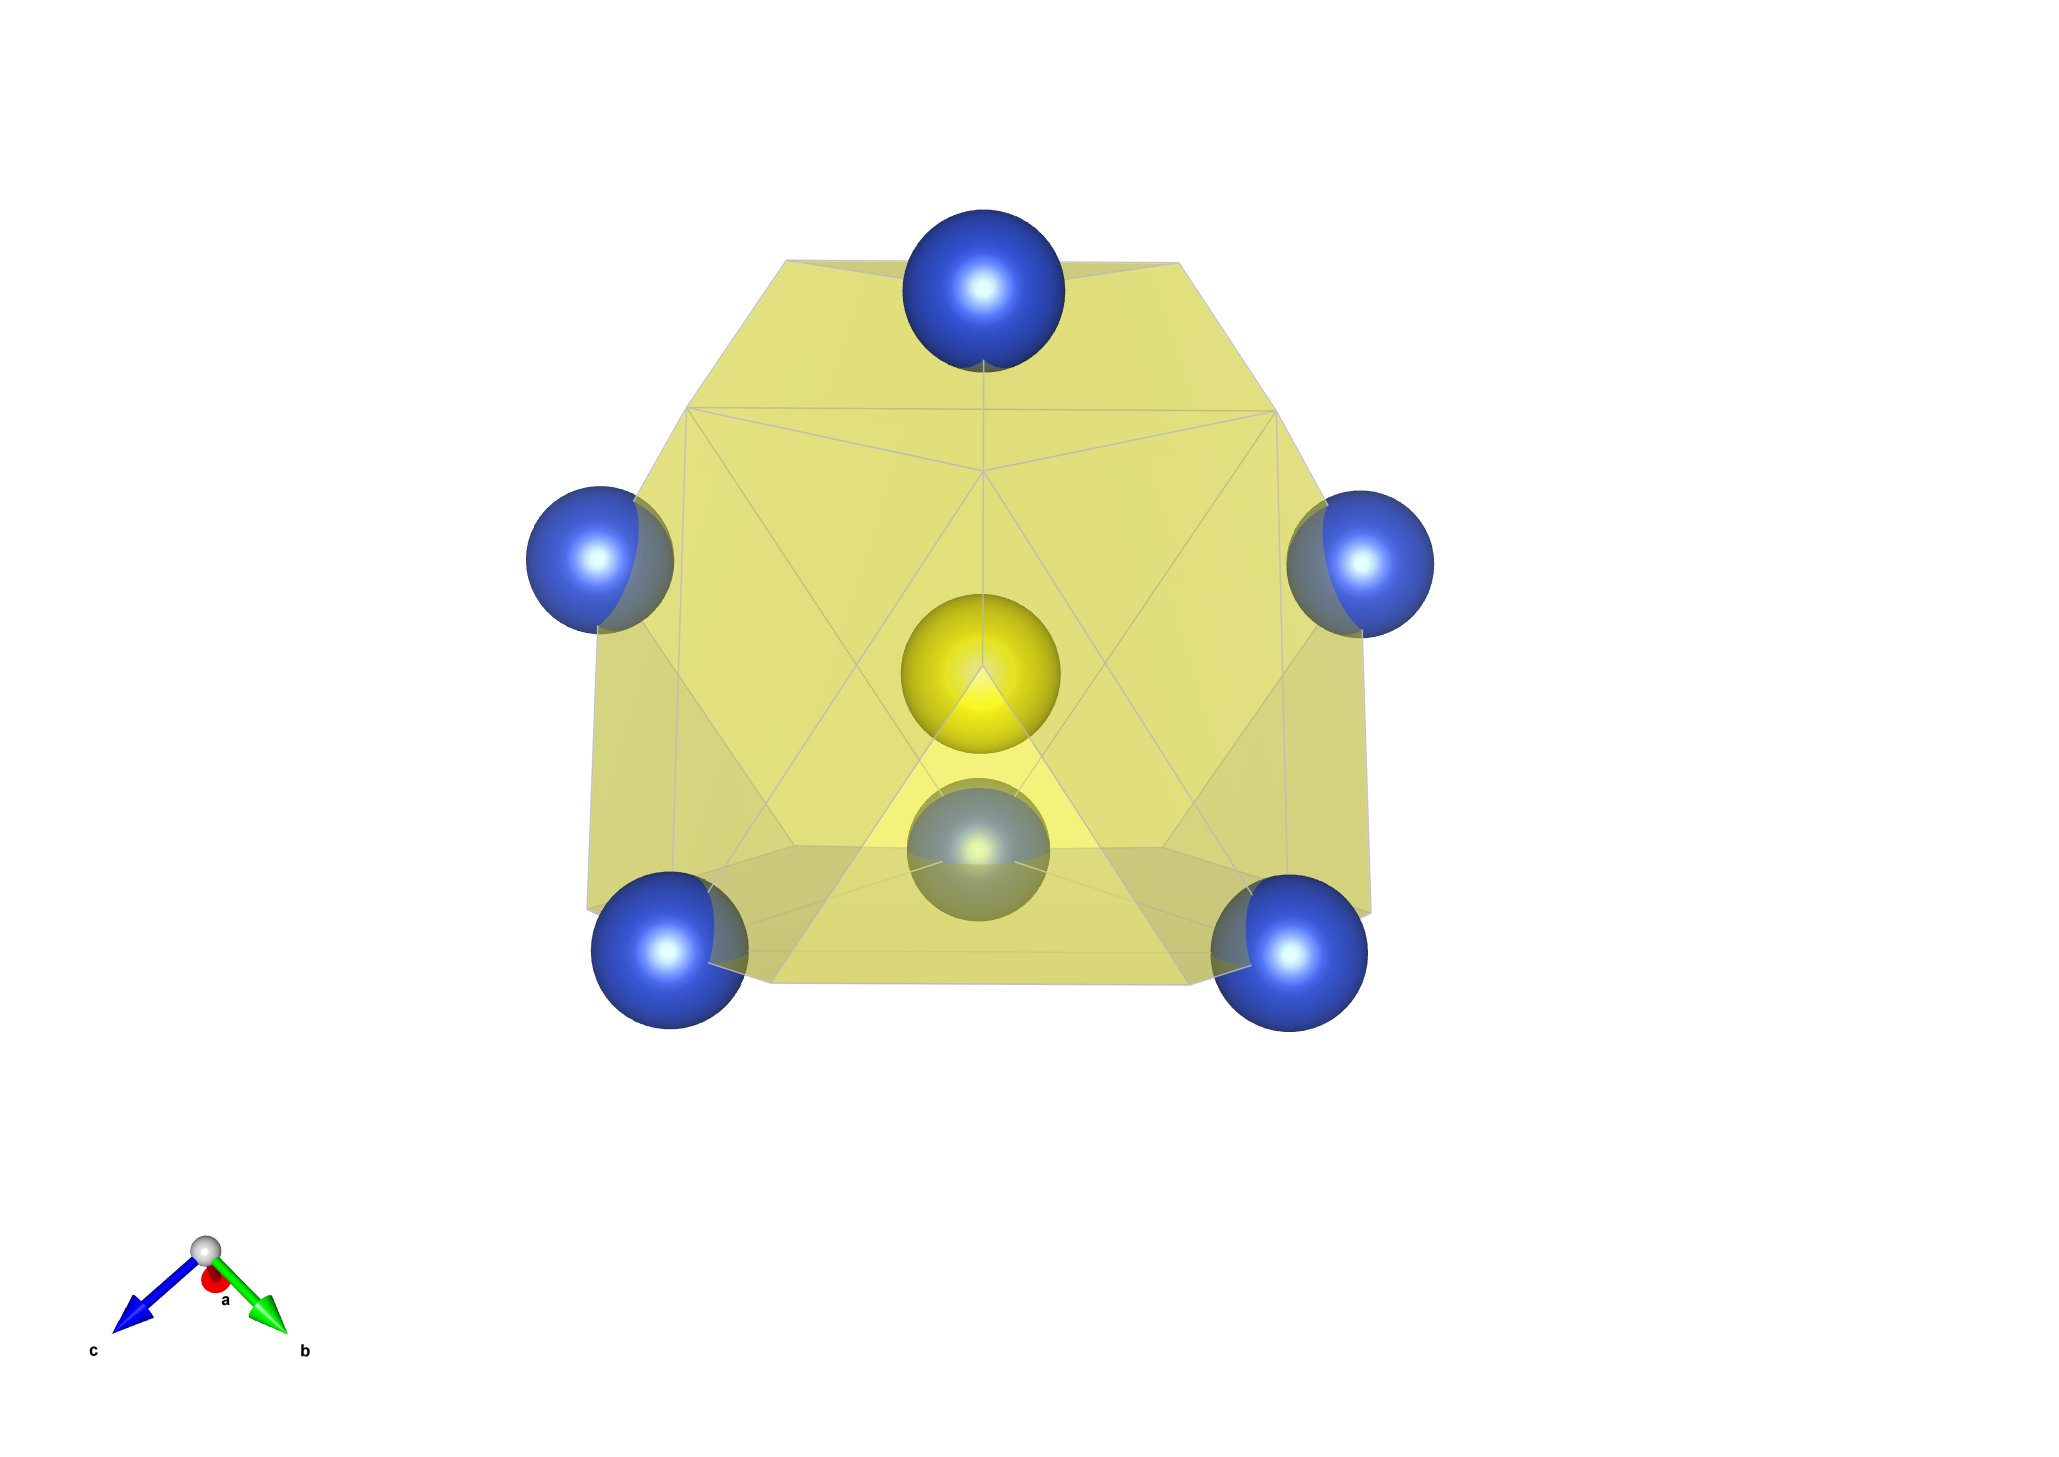
\includegraphics[width=0.9\linewidth]{var_16} \\ а)
  \end{minipage}
						\hfill
 \begin{minipage}[ht]{0.45\linewidth}\centering
    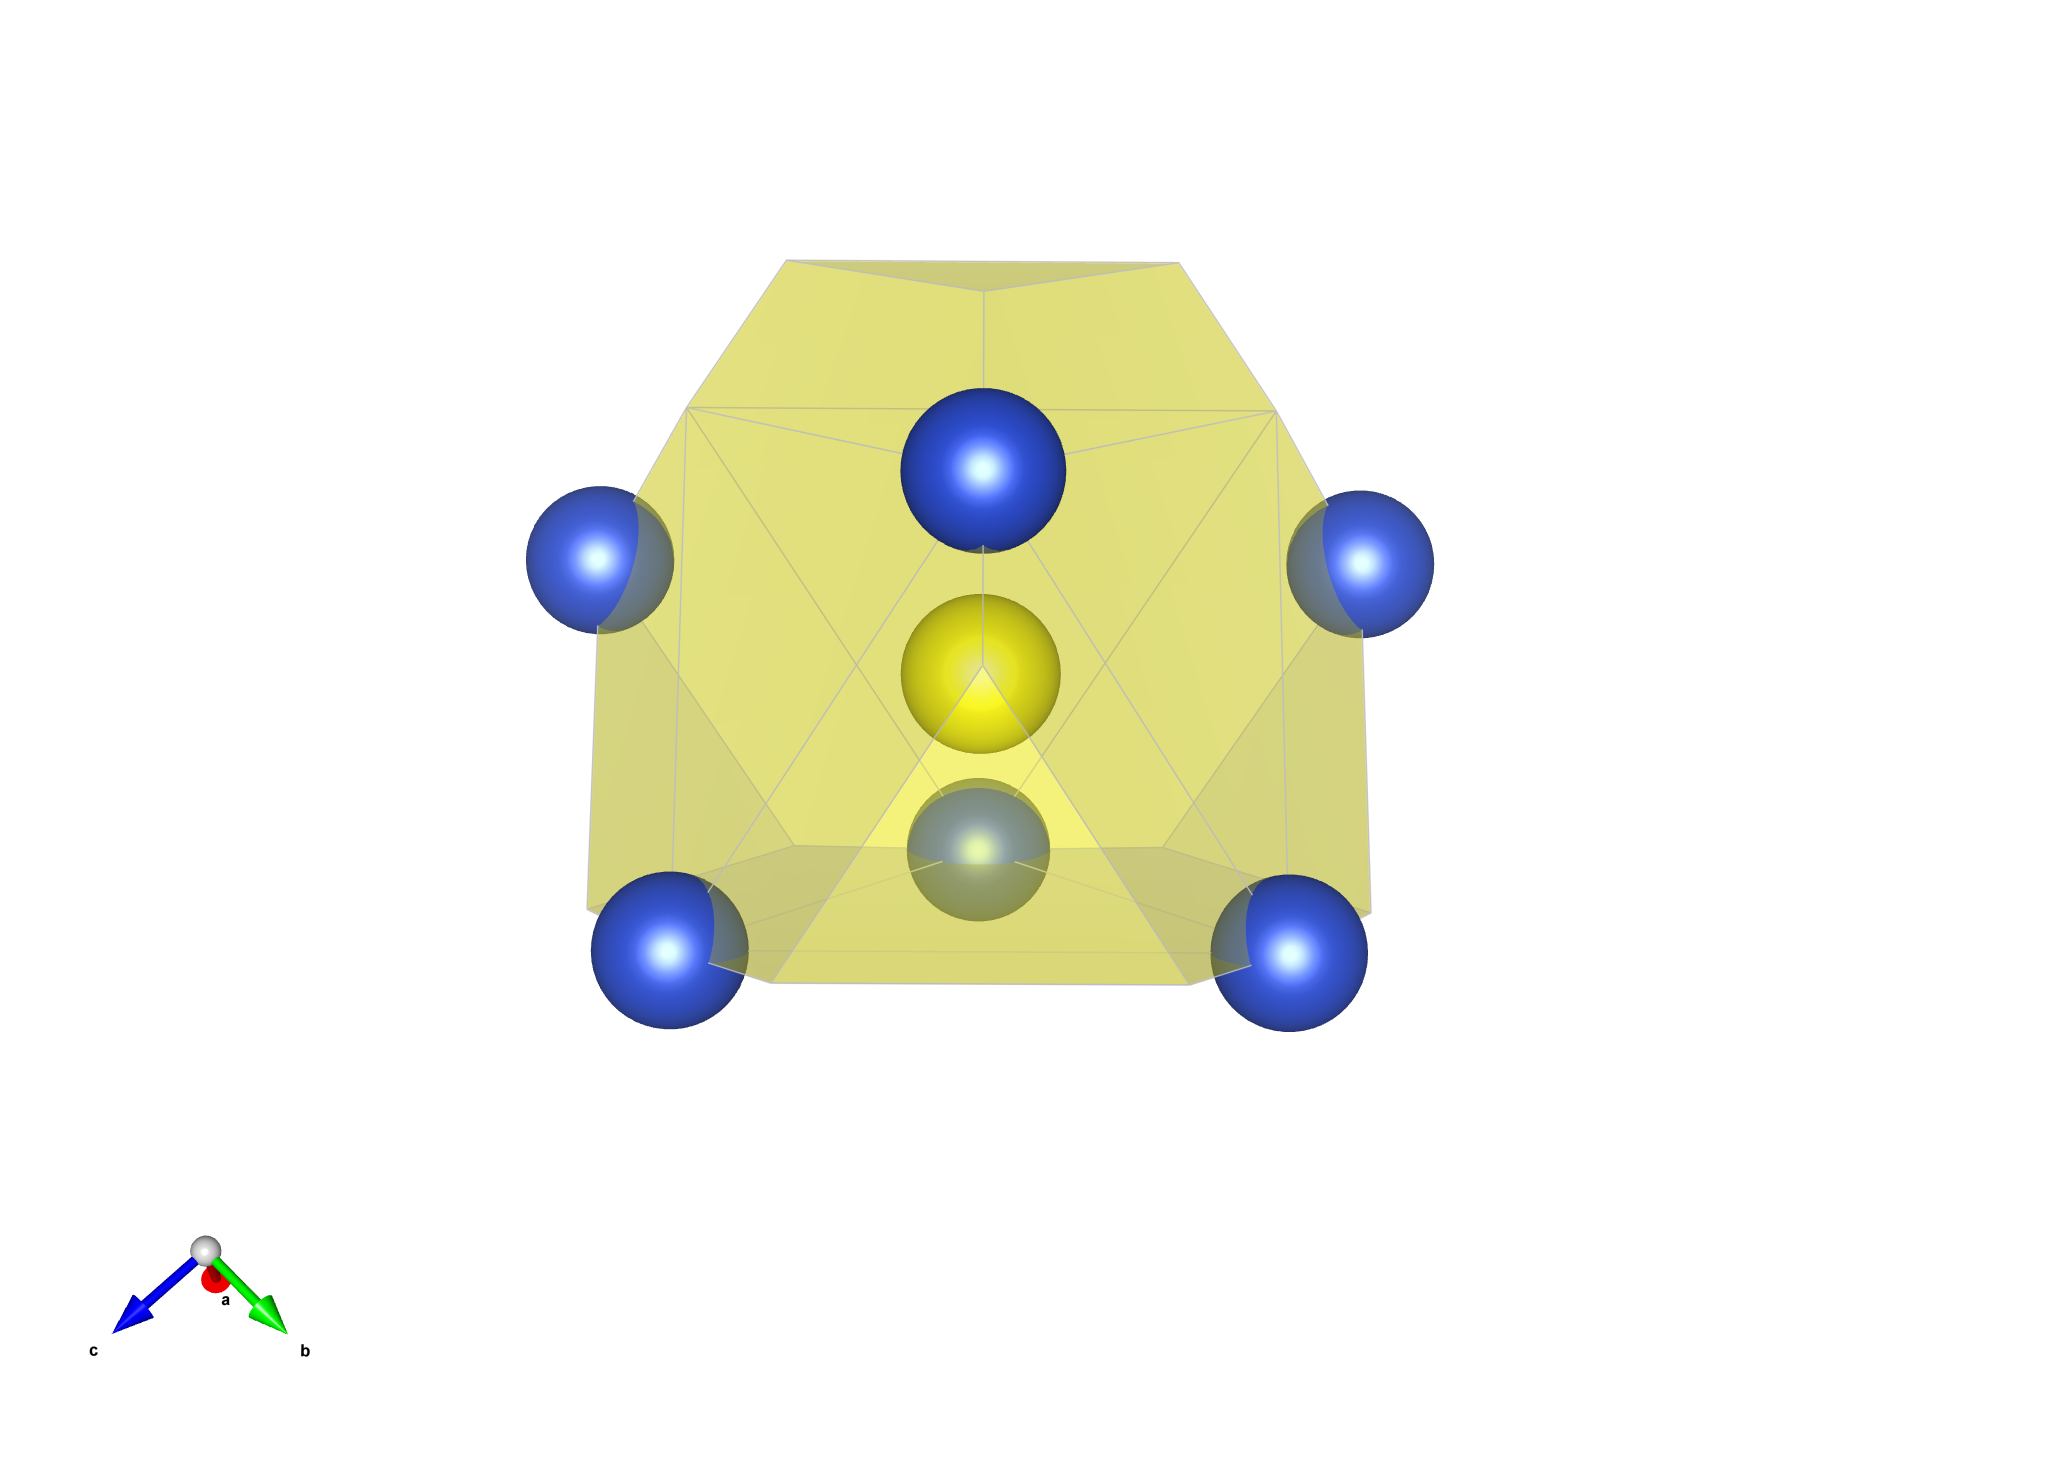
\includegraphics[width=0.9\linewidth]{var_17} \\ б)
  \end{minipage}
\vfill

  \begin{minipage}[ht]{0.45\linewidth}\centering
    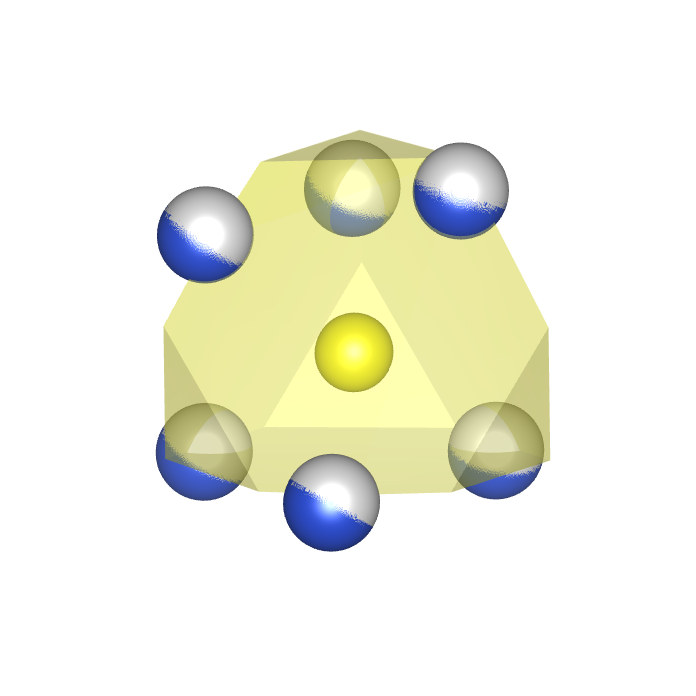
\includegraphics[width=0.9\linewidth]{var_18} \\ в)
  \end{minipage}
						\hfill
 \begin{minipage}[ht]{0.45\linewidth}\centering
    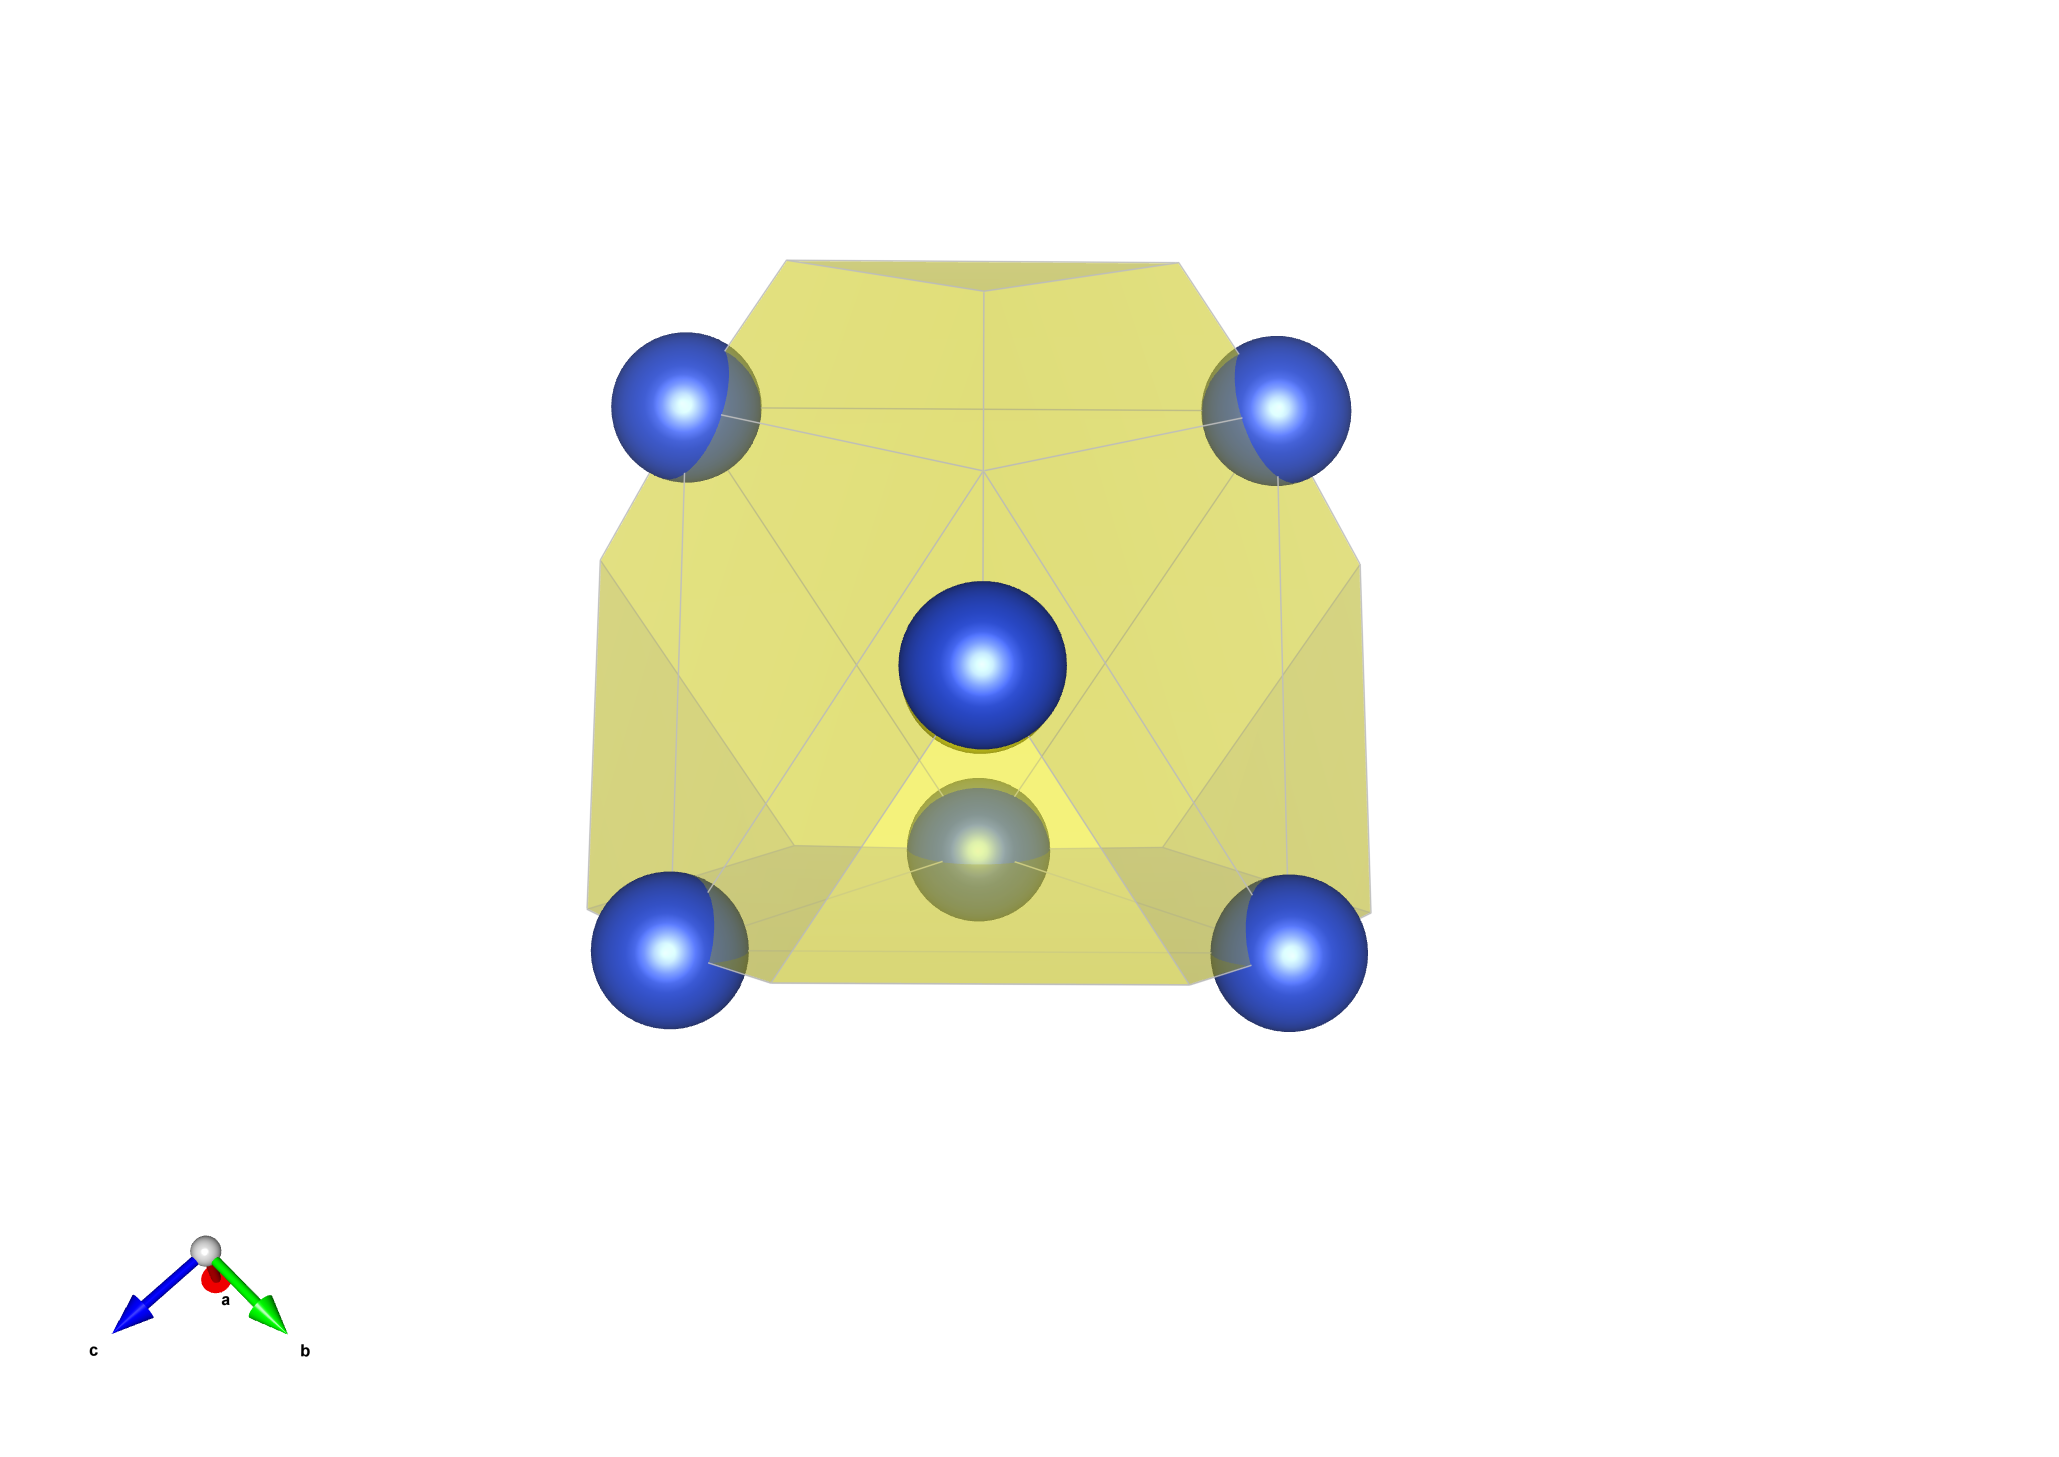
\includegraphics[width=0.9\linewidth]{var_19} \\ г)
  \end{minipage}
\vfill

  \begin{minipage}[ht]{0.45\linewidth}\centering

  \end{minipage}
						\hfill
 \begin{minipage}[ht]{0.45\linewidth}\centering

  \end{minipage}
      \caption[Изображения лавесовских полиэдров синтетического теннантита Cu\textsubscript{12}As\textsubscript{4}S\textsubscript{13}, для которых рассчитывалась энергия элементарной ячейки. Варианты с 16 по 19 включительно]{Изображения лавесовских полиэдров синтетического теннантита Cu\textsubscript{12}As\textsubscript{4}S\textsubscript{13}, для которых рассчитывалась энергия элементарной ячейки. Варианты с 16 по 19 включительно}
    \label{img:laves4}
\end{figure}



\newpage

\clearpage

\section{Особенности формирования лавесовесокого полиэдра} \label{sect3_5}

По результатам рентгеноструктурного анализа монокристаллического образца синтетического теннантита Cu\textsubscript{12}As\textsubscript{4}S\textsubscript{13} при комнатной температуре обнаружено, что значение суммы заселённостей позиций атомов Cu2 и Cu21 составляет 1, а не 1.04 как опубликовано ранее\cite{Makovicky_2006}.
Полученные результаты показывают, что на структурную формулу синтетического теннантита приходится 12 атомов меди, а не 12.5. На HAADF изображении структуры (Рис.~\ref{img:mic3}) в плоскости (011) не обнаружено дислокаций, двойникования и других дефектов структуры.
Таким образом, лавесовский полиэдр состоит из 6 атомов меди.
Разное значение эллиптичности рядов, определенное при анализе плоскости (011) атомарного изображения монокристаллического образца синтетического теннантита Cu\textsubscript{12}As\textsubscript{4}S\textsubscript{13} (Рис.~\ref{img:mic}), говорит в пользу существования позиции меди Cu21 в структуре теннантита, что согласуется с результатами рентгеноструктурного анализа описанного выше.

\begin{figure}[h]
\centering
  \begin{minipage}[ht]{0.7\linewidth}\centering
    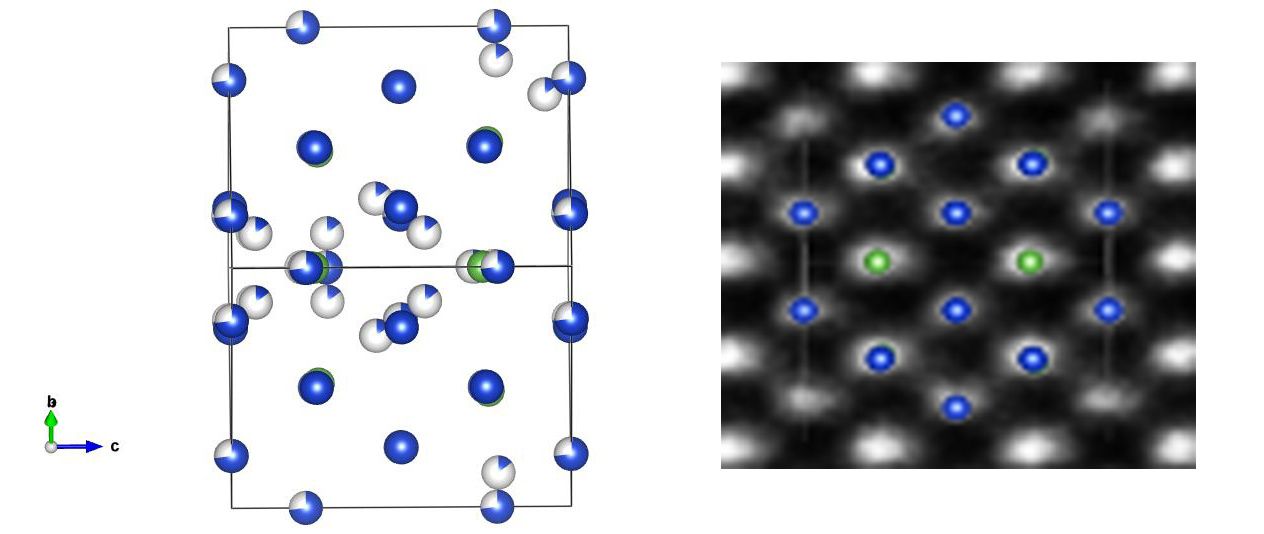
\includegraphics[width=0.9\linewidth]{mic_cu12as4s13_110} \\
  \end{minipage}

  \caption[HAADF изображение и теоретическая форма изображения рядов для образца Cu\textsubscript{12}As\textsubscript{4}S\textsubscript{13}]{HAADF изображение и теоретическая форма изображения рядов для образца Cu\textsubscript{12}As\textsubscript{4}S\textsubscript{13}}
    \label{img:mic3}
\end{figure}

На рисунке~\ref{img:xray} представлены: величина заселённости позиций атома Cu2 и изменение значения коэффициента атомарного смещения для позиции атома S2 в диапазоне температур от 85 до 293~К. Аномальное изменение значения коэффициента атомарного смещения для позиции атома S2, показывает наличие фазового перехода второго рода в диапазоне от 115 до 180 К.

\begin{figure}[ht]
  \begin{minipage}[ht]{0.5\linewidth}\centering
    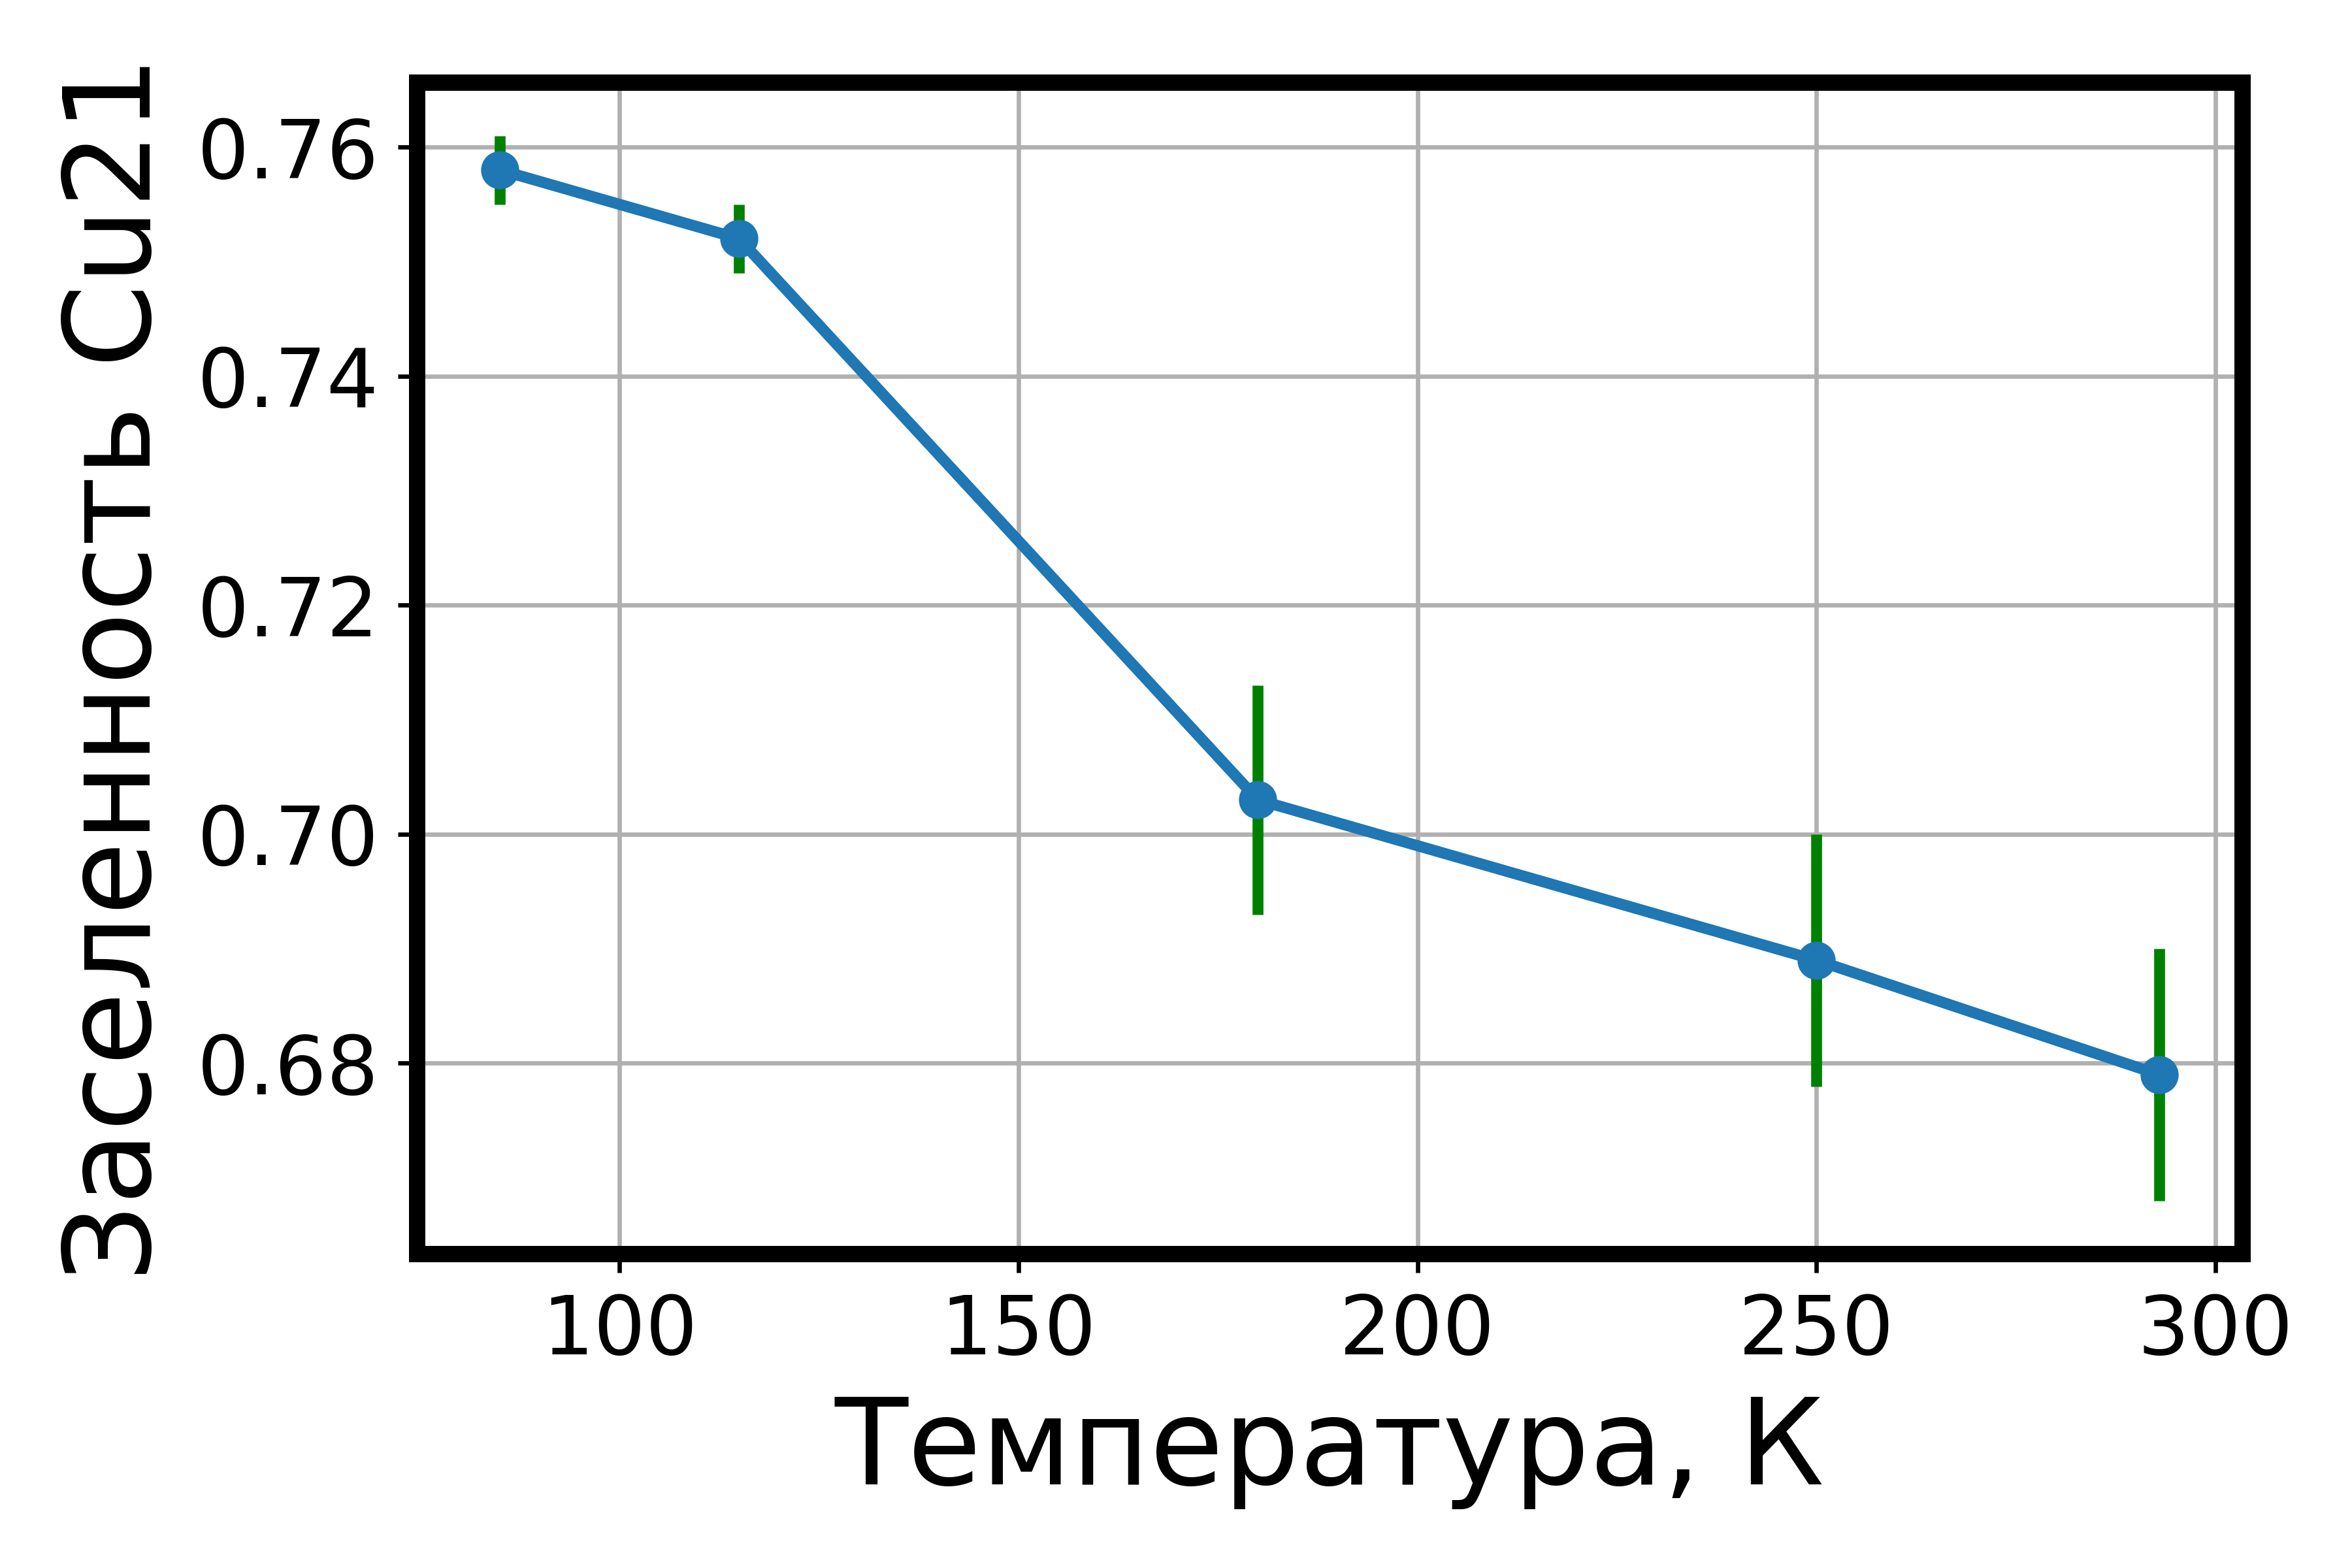
\includegraphics[width=0.9\linewidth]{structure_occCu2} \\ а)
  \end{minipage}
  \hfill
  \begin{minipage}[ht]{0.5\linewidth}\centering
    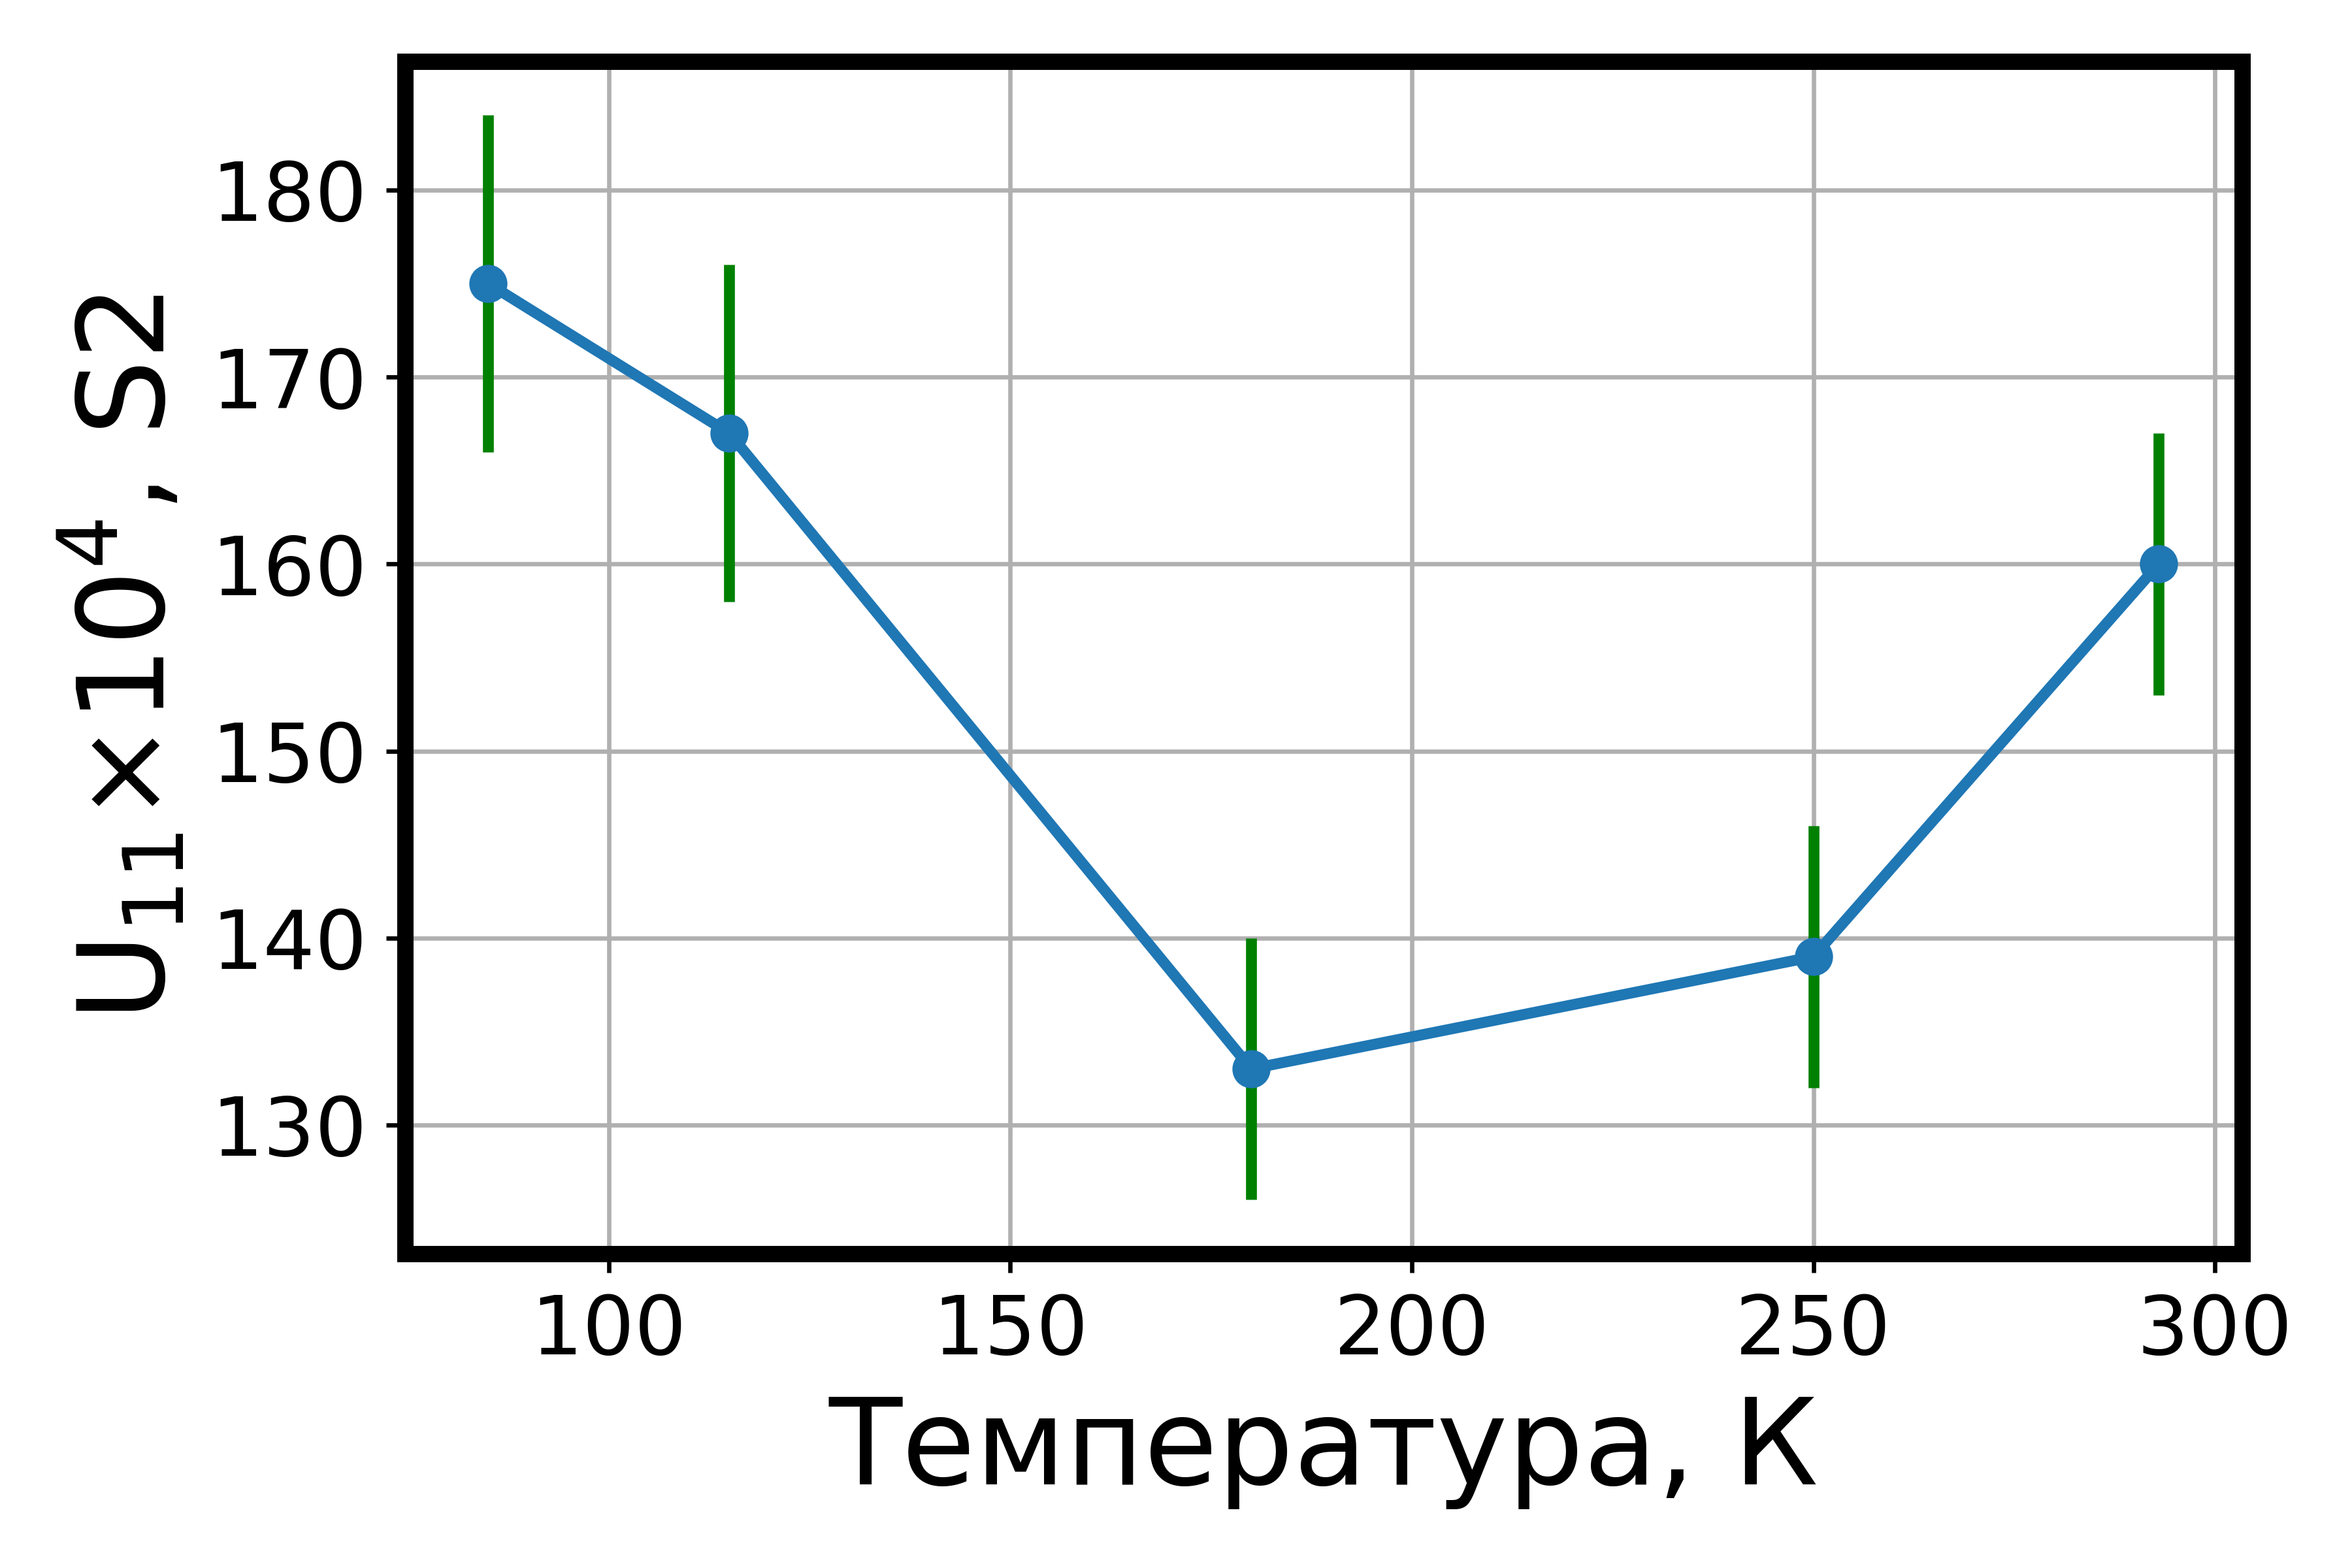
\includegraphics[width=0.9\linewidth]{structure_Ueq} \\ б)
  \end{minipage}

      \caption[Значение заселённости позиции атома Cu2 (а) и изменение значения коэффициента атомарного смещения для позиции атома S2 (б) в диапазоне температур от 85 до 293~К синтетического теннантита Cu\textsubscript{12}As\textsubscript{4}S\textsubscript{13}]{Значение заселённости позиции атома Cu2 (а) и изменение значения коэффициента атомарного смещения для позиции атома S2 (б) в диапазоне температур от 85 до 293~К синтетического теннантита Cu\textsubscript{12}As\textsubscript{4}S\textsubscript{13}}
    \label{img:xray}
\end{figure}

Рисунок \ref{img:xray2} представляет собой изображения распределений электронной плотности синтетического теннантита Cu\textsubscript{12}As\textsubscript{4}S\textsubscript{13} при температуре 293~(а) и 85~(б)~К в плоскости (011). По форме линий электронной плотности видно, что происходит полное разделение позиций Cu2 и Cu21. При комнатной температуре расстояние между Cu2 и Cu21 составляет 1.027(6)~$\angstrom$, при 85~К --- 1.108(5)~$\angstrom$. Расчёт энергий ФМ, АФМ, ПМ и диамагнитного состояний для экспериментально полученных структур показывает, что АФМ упорядочение в экспериментальной структуре при 85~К энергетически более выгодно, чем ферро- или пара- или диамагнитное состояния при этой же температуре. Для экспериментальной структуры при 293~К ФМ, АФМ, ПМ конфигурации имеют одинаковую (до 4 знака) энергию, что указывает на их одинаковую вероятность.

\begin{figure}[ht]
  \begin{minipage}[ht]{0.5\linewidth}\centering
    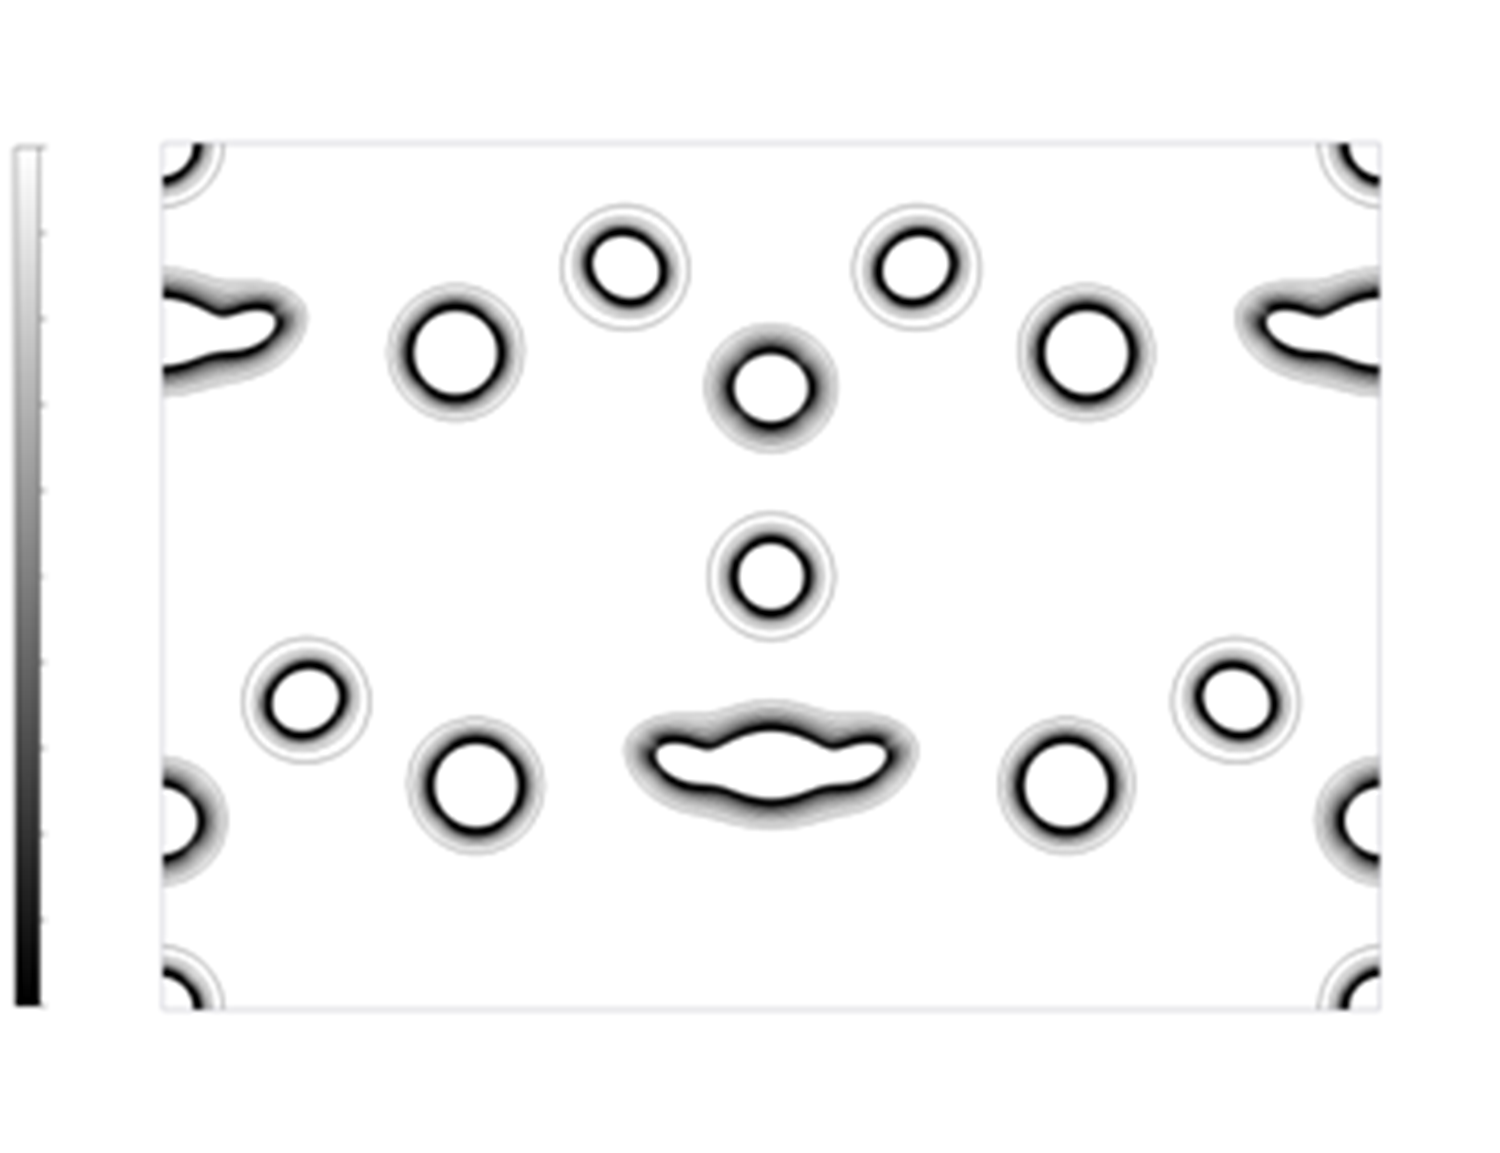
\includegraphics[width=0.9\linewidth]{Electron_density_293.png} \\ а)
  \end{minipage}
  \hfill
  \begin{minipage}[ht]{0.5\linewidth}\centering
    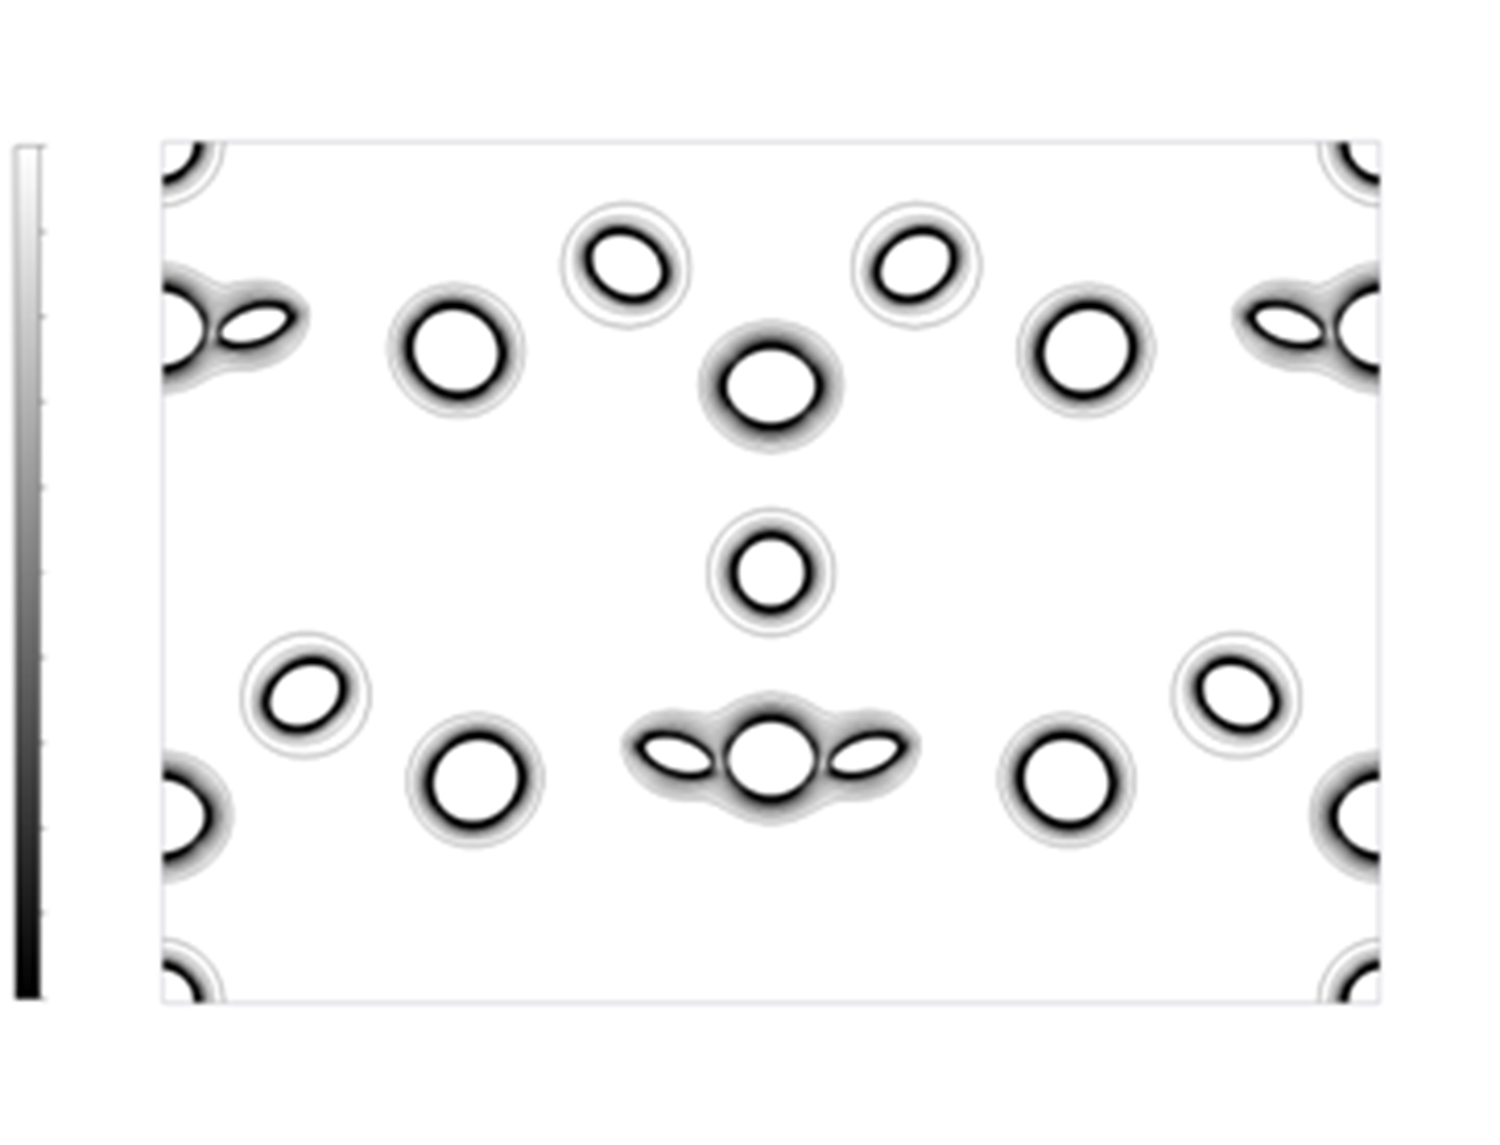
\includegraphics[width=0.9\linewidth]{Electron_density_85.png} \\ б)
  \end{minipage}

      \caption[Распределение электронной плотности при температуре 293~(а) и 85~(б)~К в плоскости (011) синтетического теннантита Cu\textsubscript{12}As\textsubscript{4}S\textsubscript{13}]{Распределение электронной плотности при температуре 293~(а) и 85~(б)~К в плоскости (011) синтетического теннантита Cu\textsubscript{12}As\textsubscript{4}S\textsubscript{13}}
    \label{img:xray2}
\end{figure}


По данным первопринципных расчётов энергий элементарных ячеек для синтетического теннантита Cu\textsubscript{12}As\textsubscript{4}S\textsubscript{13} следует,  что смещение атома меди в лавесовсом полиэдре может приводить как к увеличению энергии ячейки, так и к её уменьшению.
Результаты показывают, что существующее неэквивалентное  окружение атомов меди в позициях Cu21 и Cu2 ведет к возникновению разного химического потенциала для структур с разным расположением атомов меди (анализировались позиции Cu21 и Cu2) и, вероятно, является движущей силой для возникновения позиции Cu21. Расстояние между сдвинутым атомом и его идеальным положением в лавесовсом полиэдре для наиболее энергетически выгодной элементарной ячейки составляет 0.6~$\angstrom$, по экспериментальным данным --- 1.027(6)~$\angstrom$.
Анализ распределения электрических зарядов указывает, что для более выгодных с энергетической точки зрения структур не возникает разной валентности на атомах меди Cu1,
но появляется разность зарядов для позиций атомов Cu2 (Cu21) (варианты структур с 11 по 15). Также стоит отметить, что структуры, где сдвинуты все 6 атомов меди, обладают большей энергией элементарной ячейки в сравнении с энергией идеального полиэдра и представляют не самые энергетически выгодные конфигурации  (варианты 5--10).










\clearpage

\newpage


\section{Выводы по Главе 3} \label{sect3_6}

В третьей главе представлены результаты исследования структуры синтетического теннантита.

% Результаты этой работы показывают, что модель описания синтетического теннатита не схожа с изоморфным аналогом тетраэжритом. Так же обнаружено, что механиз фазового перехода сдвигается с 124 до 84 притом, что механизм описания перехода отличается от механизма тетраэдрита
% Особое внимание уделено анализу возможных структурных политипов для проверки идеи наличия статистически разориентированных позиций атомов меди.


По результатам рентгеноструктурного анализа монокристаллического образца синтетического теннантита Cu\textsubscript{12}As\textsubscript{4}S\textsubscript{13} при комнатной температуре обнаружено, что значение суммы заселенностей позиций атомов Cu2 и Cu21 составляет 1, а не 1.04 как опубликовано ранее\cite{Makovicky_2006}.

По данным первопринципных расчётов энергий элементарных ячеек для синтетического теннантита Cu\textsubscript{12}As\textsubscript{4}S\textsubscript{13} следует,  что смещение атома меди в лавесовском полиэдре может приводить как к увеличению энергии ячейки, так и к уменьшению.
Результаты показывают, что существующее неэквивалентное  окружение атомов меди в позициях Cu21 и Cu2 ведет к отличию химического потенциала для структур с разным расположением атомов меди (анализировались позиции Cu21 и Cu2), появлению ассиметричных связей As(CuS\textsubscript{3})As и, вероятно, является движущей силой для возникновения позиции Cu21. В следствии этого процесса происходит размягчение фононных мод в структуре синтетического теннантита.

Таким образом:
\begin{enumerate}
  \item Cинтетический теннантит Сu\textsubscript{12}As\textsubscript{4}S\textsubscript{13} обладает неэквивалентным  окружением атомов меди в позициях Cu21 и Cu2, а в элементарной ячейке содержит 12 атомов меди.
  \item Неэквивалентные позиции атомов меди Cu21 и Cu2 в синтетическом теннантите способствуют появлению ассиметричных связей As(CuS\textsubscript{3})As, которые приводят к размягчению фононных мод в структуре синтетического теннантита Сu\textsubscript{12}As\textsubscript{4}S\textsubscript{13}.
\end{enumerate}
% Наличие рядов меди с электронной плотностью в форме эллипса, определенное после анализа плоскости (011) атомарного изображения монокристаллического образца синтетического теннантита Cu\textsubscript{12}As\textsubscript{4}S\textsubscript{13}, показывает существование позиции атома меди Cu21 и согласуется с результатами рентгеноструктурного анализа, описанного выше.
% 
% 
% 
% Расстояние между сдвинутым атомом и его идеальным положением в лавесовском полиэдре составляет для наиболее энергетически выгодной элементарной ячейки 0.6~$\angstrom$, по экспериментальным данным --- 1.027(6)~$\angstrom$.
% Анализ распределения электрических зарядов показывает, что для более выгодных с энергетической точки зрения структур не возникает разной валентности на атомах меди Cu1,
% но появляется разность зарядов для позиций атомов Cu2 (Cu21).
% 
% Расчёт энергий ФМ, АФМ, ПМ и диамагнитного состояний для экспериментально полученных структур показывает, что АФМ упорядочение в экспериментальной структуре при 85~К энергетически более выгодно, чем ферро-, пара- или диамагнитное состояния при этой же температуре.

\newpage
